\documentclass[12pt, a4paper]{report}

% ------------------------------------------------------------
\usepackage[utf8]{inputenc}
\usepackage[T1]{fontenc}
\usepackage[catalan, provide=*]{babel}
\usepackage{microtype}
\usepackage{pdfpages}
\usepackage{graphicx}
\usepackage{float}

% ------------------------------------------------------------
\usepackage[
  top=2.5cm, bottom=2.5cm,
  left=3cm,  right=2.5cm,
  headheight=15pt
]{geometry}

% ------------------------------------------------------------
%  COLORS — paleta neutra académica
% ------------------------------------------------------------
\usepackage[dvipsnames,table]{xcolor}

\definecolor{darkblue}{RGB}{26,58,92}       % títols
\definecolor{midblue}{RGB}{55,90,130}       % seccions
\definecolor{textgray}{RGB}{60,60,60}       % text secundari
\definecolor{lightgray}{RGB}{245,245,245}   % fons taules
\definecolor{rulegray}{RGB}{195,195,195}    % línies
\definecolor{codebg}{RGB}{248,248,248}
\definecolor{codeframe}{RGB}{210,210,210}
\definecolor{accentgreen}{RGB}{38,100,55}
\definecolor{accentred}{RGB}{150,35,35}
% boxes
\definecolor{infoback}{RGB}{238,245,252}
\definecolor{infoframe}{RGB}{55,90,130}
\definecolor{warnback}{RGB}{254,248,238}
\definecolor{warnframe}{RGB}{170,95,20}
\definecolor{resultback}{RGB}{238,250,242}
\definecolor{resultframe}{RGB}{38,100,55}

% ------------------------------------------------------------
%  FONTS
% ------------------------------------------------------------
\usepackage{palatino}
\usepackage[scaled=0.90]{helvet}
\usepackage{courier}

% ------------------------------------------------------------
%  CAPCALERES
% ------------------------------------------------------------
\usepackage{fancyhdr}
\pagestyle{fancy}
\fancyhf{}
\fancyhead[L]{\small\sffamily\color{textgray}\leftmark}
\fancyhead[R]{\small\sffamily\color{textgray}Neil Pradas Martínez \textperiodcentered{} TFG 2025/26}
\fancyfoot[C]{\small\color{textgray}\thepage}
\renewcommand{\headrulewidth}{0.3pt}
\renewcommand{\headrule}{%
  \hbox to\headwidth{\color{rulegray}\leaders\hrule height 0.3pt\hfill}}
\renewcommand{\footrulewidth}{0pt}

% ------------------------------------------------------------
%  TÍTOLS
% ------------------------------------------------------------
\usepackage{titlesec}

\titleformat{\chapter}[display]
  {\normalfont\sffamily\huge\color{darkblue}}
  {\normalfont\sffamily\small\color{textgray}\MakeUppercase{\chaptertitlename}\ \thechapter}
  {6pt}{\huge}
\titlespacing*{\chapter}{0pt}{-8pt}{18pt}

\titleformat{\section}
  {\normalfont\sffamily\large\bfseries\color{darkblue}}
  {\thesection}{1em}{}
  [\vspace{-3pt}{\color{rulegray}\hrule height 0.3pt}\vspace{2pt}]

\titleformat{\subsection}
  {\normalfont\sffamily\normalsize\bfseries\color{midblue}}
  {\thesubsection}{1em}{}

\titleformat{\subsubsection}
  {\normalfont\normalsize\bfseries\color{textgray}}
  {\thesubsubsection}{1em}{}

% ------------------------------------------------------------
%  TAULES
% ------------------------------------------------------------
\usepackage{booktabs}
\usepackage{tabularx}
\usepackage{longtable}
\usepackage{multirow}
\usepackage{array}
\newcolumntype{L}[1]{>{\raggedright\arraybackslash}p{#1}}
\newcolumntype{C}[1]{>{\centering\arraybackslash}p{#1}}
\newcolumntype{R}[1]{>{\raggedleft\arraybackslash}p{#1}}

% ------------------------------------------------------------
%  FIGURES
% ------------------------------------------------------------
\usepackage{graphicx}
\graphicspath{{./}}
\usepackage{float}
\usepackage{caption}
\usepackage{subcaption}
\captionsetup{
  font=small,
  labelfont={bf,sf,color=darkblue},
  textfont={color=textgray},
  margin=0.5cm,
  skip=5pt
}

% ------------------------------------------------------------
%  CODI
% ------------------------------------------------------------
\usepackage{listings}
\lstset{extendedchars=true}
\lstdefinestyle{python}{
  language=Python,
  backgroundcolor=\color{codebg},
  frame=single, framerule=0.4pt, rulecolor=\color{codeframe},
  basicstyle=\ttfamily\small,
  keywordstyle=\color{darkblue}\bfseries,
  commentstyle=\color{textgray}\itshape,
  stringstyle=\color{accentgreen},
  numbers=left, numberstyle=\tiny\color{textgray},
  breaklines=true, showstringspaces=false,
  tabsize=4, extendedchars=true, inputencoding=utf8
}
\lstdefinestyle{sql}{
  language=SQL,
  backgroundcolor=\color{codebg},
  frame=single, framerule=0.4pt, rulecolor=\color{codeframe},
  basicstyle=\ttfamily\small,
  keywordstyle=\color{darkblue}\bfseries,
  commentstyle=\color{textgray}\itshape,
  stringstyle=\color{accentgreen},
  breaklines=true, showstringspaces=false,
  tabsize=2
}
\lstdefinestyle{bash}{
  language=bash,
  backgroundcolor=\color{codebg},
  frame=single, framerule=0.4pt, rulecolor=\color{codeframe},
  basicstyle=\ttfamily\small,
  keywordstyle=\color{darkblue},
  commentstyle=\color{textgray}\itshape,
  breaklines=true, showstringspaces=false,
  extendedchars=true, inputencoding=utf8
}

% ------------------------------------------------------------
%  HYPERLINKS
% ------------------------------------------------------------
\usepackage[
  colorlinks=true,
  linkcolor=darkblue,
  citecolor=midblue,
  urlcolor=midblue,
  pdftitle={Predicció d'Actius Financers mitjançant ML i Anàlisi de Sentiment},
  pdfauthor={Neil Pradas Martínez},
  pdfsubject={Treball de Fi de Grau - UAB 2025/26}
]{hyperref}

% ------------------------------------------------------------
\usepackage{enumitem}
\usepackage{amsmath}
\usepackage{amssymb}
\usepackage{parskip}
\usepackage{setspace}
\usepackage{tcolorbox}
\tcbuselibrary{skins, breakable}

% Control de vídues i orfes (evita línies soltes a inici/final de pàgina)
\widowpenalty=10000
\clubpenalty=10000
\displaywidowpenalty=10000
\brokenpenalty=10000

% ------------------------------------------------------------
%  CAIXES
% ------------------------------------------------------------
% Estil "admonition" acadèmic (ETH/IEEE): fons gris molt clar, cantonades
% rectes, només una fina línia lateral en color sobri, sense ombres ni farciment
% de color saturat. La distinció entre tipus la dona el filet lateral i el títol.
\newtcolorbox{infobox}[1][]{
  enhanced, breakable, sharp corners,
  colback=lightgray, colframe=darkblue,
  boxrule=0pt, leftrule=2.5pt,
  left=9pt, right=9pt, top=5pt, bottom=5pt,
  fonttitle=\small\sffamily\bfseries\color{darkblue}, coltitle=darkblue,
  title={#1},
  before skip=9pt, after skip=9pt
}
\newtcolorbox{warningbox}[1][]{
  enhanced, breakable, sharp corners,
  colback=lightgray, colframe=accentred,
  boxrule=0pt, leftrule=2.5pt,
  left=9pt, right=9pt, top=5pt, bottom=5pt,
  fonttitle=\small\sffamily\bfseries\color{accentred}, coltitle=accentred,
  title={#1},
  before skip=9pt, after skip=9pt
}
\newtcolorbox{resultbox}[1][]{
  enhanced, breakable, sharp corners,
  colback=lightgray, colframe=accentgreen,
  boxrule=0pt, leftrule=2.5pt,
  left=9pt, right=9pt, top=5pt, bottom=5pt,
  fonttitle=\small\sffamily\bfseries\color{accentgreen}, coltitle=accentgreen,
  title={#1},
  before skip=9pt, after skip=9pt
}

% ============================================================
\begin{document}
\setstretch{1.15}

% ------------------------------------------------------------
%  PORTADA
% ------------------------------------------------------------
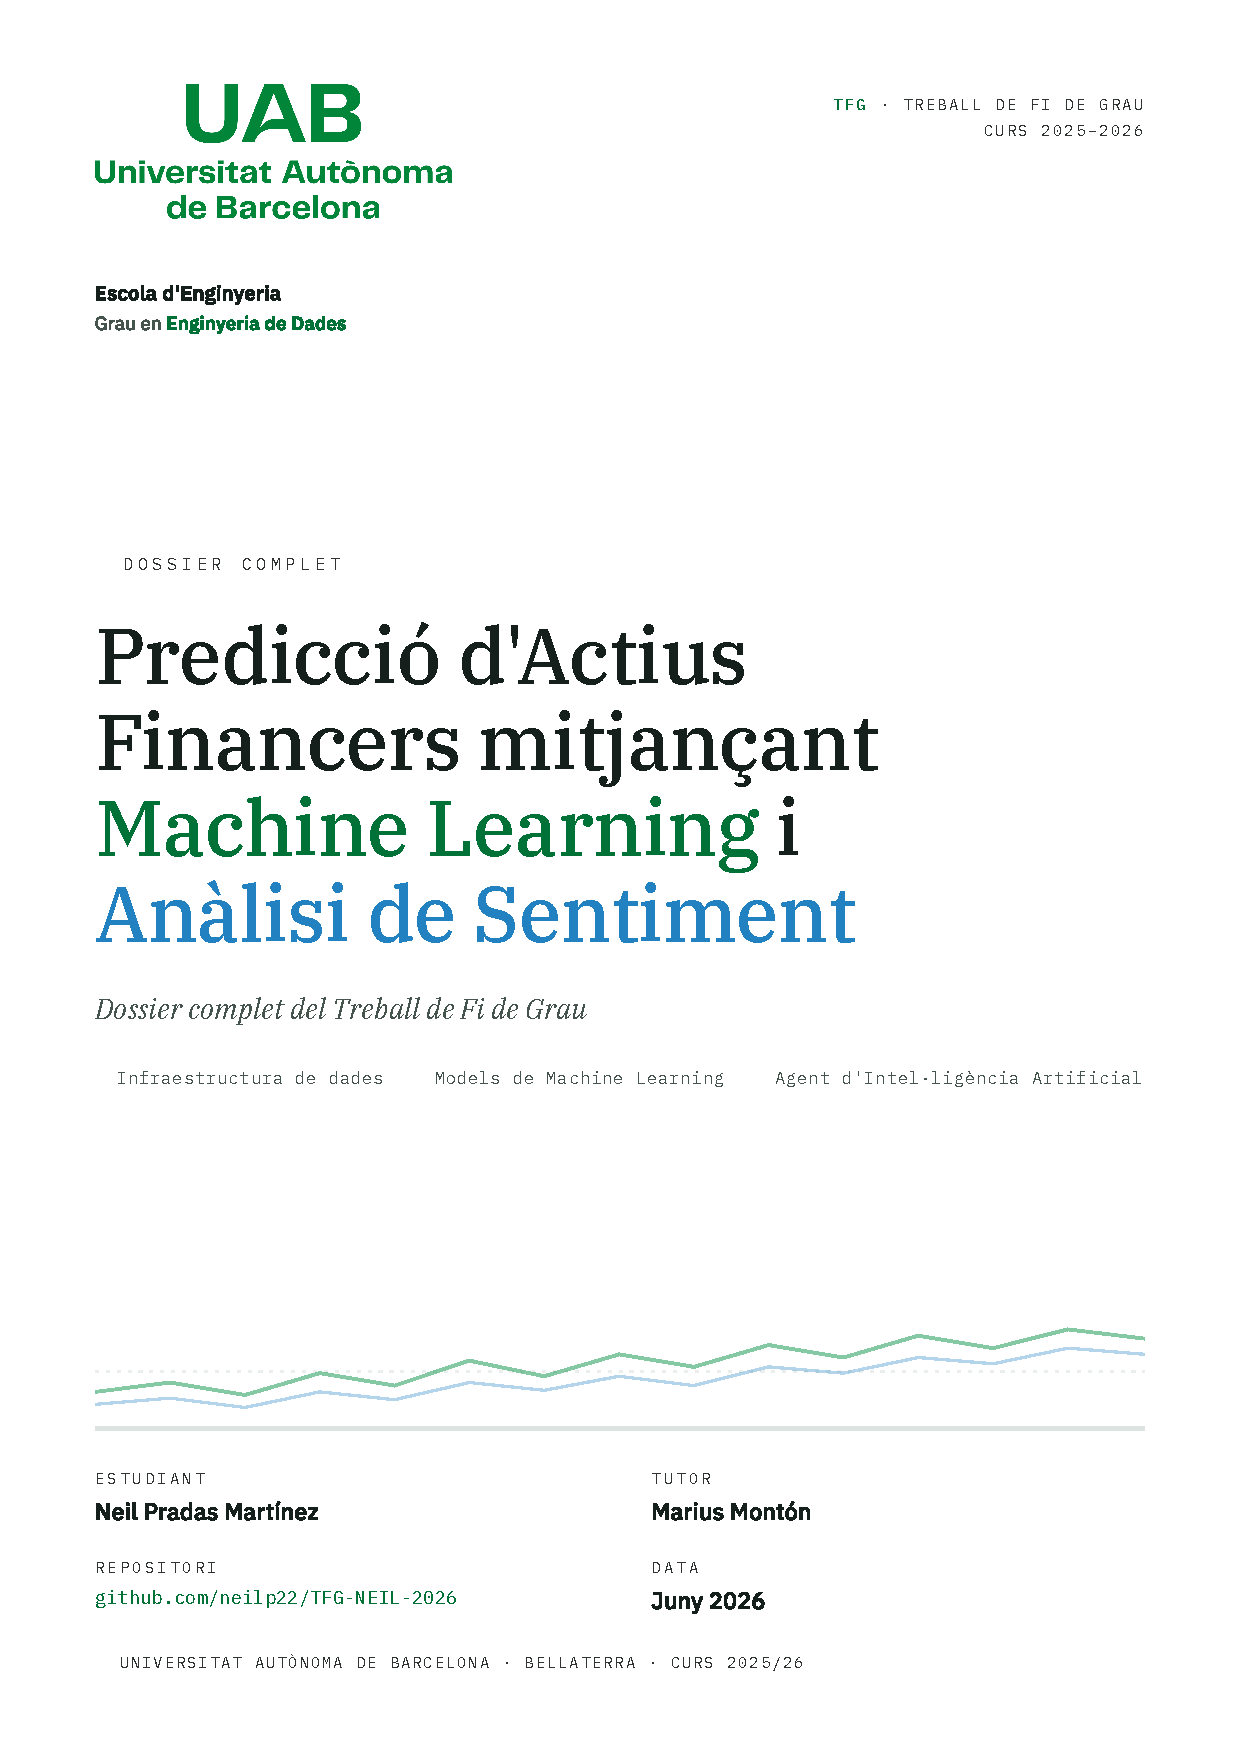
\includepdf{portada.pdf}

% ------------------------------------------------------------
%  RESUM / ABSTRACT
% ------------------------------------------------------------
\chapter*{Resum}
\addcontentsline{toc}{chapter}{Resum}
\begingroup\setstretch{1.0}

Aquest Treball de Fi de Grau aborda una pregunta central de les finances computacionals: pot un sistema d'aprenentatge automàtic, enriquit amb anàlisi de sentiment de notícies financeres, predir la direcció diària del preu de Bitcoin amb significança estadística? Per respondre-la s'ha construït una infraestructura completa i reproduïble: una base de dades PostgreSQL amb 12 taules, un corpus de 105.125 notícies (2011--2026) processades amb FinBERT, 65.466 registres OHLCV de Binance i un pipeline d'actualització automàtica diària.

Quatre famílies de models (ARIMA, XGBoost, LightGBM i LSTM) s'han avaluat amb validació \textit{walk-forward} amb embargament temporal, tests de significança i intervals de confiança al 95\%, després d'una auditoria que va detectar i corregir 10 problemes metodològics del pipeline. El resultat és un \textit{null finding} estadísticament honest: cap model supera l'atzar (millor AUC = 0,532; $p = 0{,}287$; IC 95\% que inclou 0,5), consistent amb la hipòtesi d'eficiència semi-forta del mercat. Com a troballa original, l'experiment de causalitat inversa mostra que el sentiment de les notícies matinals és sistemàticament més informatiu que l'agregat diari, evidència que part del senyal aparent del sentiment en la literatura pot ser un artefacte: les notícies descriuen el preu més que no pas l'anticipen.

Sobre aquesta base, la segona fase del treball construeix un \textbf{sistema multi-agent} d'IA sobre GPT-4o que integra senyals heterogènies i comunica explícitament la seva incertesa. El sistema combina tres rols especialitzats: un \textit{Analista} (\textit{function calling} amb 13 eines, RAG amb FAISS i un \textit{Confluence Score} calibrat empíricament), un \textit{Risk Manager} adversarial que audita l'anàlisi i un \textit{Decision Maker} que fusiona totes les fonts en una decisió final GO/NO-GO; aquesta decisió es pren amb un \textbf{motor de regles determinista} (verificació en codi, reproduïble) mentre que el LLM només n'aporta la component qualitativa. El sistema s'ha avaluat per tres vies: mètriques RAGAS (Faithfulness 0,863), un estudi d'ablació LLM de 365 dies amb 500 trucades reals, i l'auditoria de \textit{leakage} del model integrat. Es completa amb un dashboard web de transparència total i un bot de \textit{paper trading} connectat per API a Bybit Demo, que ha executat operacions reals (en compte de pràctiques) amb gestió de risc automàtica (\textit{stop loss}/\textit{take profit} natius, \textit{break-even} i \textit{trailing stop}). Tanmateix, en ser una avaluació en una finestra temporal curta i impossible de \textit{backtestejar} sense contaminació, es conclou que el sistema funciona correctament a nivell d'enginyeria però que encara no es pot afirmar el seu rendiment amb significança estadística: l'avaluació en viu prolongada és la línia de continuació natural.

\paragraph{Paraules clau:} Bitcoin, aprenentatge automàtic, anàlisi de sentiment, FinBERT, hipòtesi d'eficiència de mercat, agents LLM, RAG, validació walk-forward.
\endgroup

\chapter*{Abstract}
\addcontentsline{toc}{chapter}{Abstract}
\begingroup\setstretch{1.0}

This Bachelor's Thesis addresses a central question in computational finance: can a machine learning system, enriched with sentiment analysis of financial news, predict the daily direction of Bitcoin's price with statistical significance? To answer it, a complete and reproducible infrastructure was built: a PostgreSQL database with 12 tables, a corpus of 105,125 news items (2011--2026) processed with FinBERT, 65,466 OHLCV records from Binance, and a fully automated daily update pipeline.

Four model families (ARIMA, XGBoost, LightGBM, and LSTM) were evaluated using walk-forward validation with a temporal embargo, significance tests, and 95\% confidence intervals, after an audit that detected and corrected 10 methodological issues in the pipeline. The outcome is a statistically honest null finding: no model beats chance (best AUC = 0.532; $p = 0.287$; 95\% CI including 0.5), consistent with the semi-strong form of the Efficient Market Hypothesis. As an original contribution, the reverse-causality experiment shows that morning news sentiment is systematically more informative than the full-day aggregate, providing evidence that part of the apparent sentiment signal in the literature may be an artifact: news describes price movements rather than anticipating them.

Building on this, the second phase develops a \textbf{multi-agent AI system} on top of GPT-4o that integrates heterogeneous signals and explicitly communicates its uncertainty. It combines three specialised roles: an \textit{Analyst} (function calling with 13 tools, FAISS-based RAG, and an empirically calibrated Confluence Score), an adversarial \textit{Risk Manager} that audits the analysis, and a \textit{Decision Maker} that fuses all sources into a final GO/NO-GO decision; this decision is produced by a \textbf{deterministic rule engine} (code-based, reproducible verification) while the LLM only contributes the qualitative component. The system was evaluated through three complementary routes: RAGAS metrics (Faithfulness 0.863), a 365-day LLM ablation study with 500 real API calls, and a leakage audit of the integrated ML model. It is completed by a full-transparency web dashboard and a paper trading bot connected via API to Bybit Demo, which has executed real (demo-account) trades with automatic risk management (native stop loss/take profit, break-even and trailing stop). However, since this is an evaluation over a short time window that cannot be backtested without contamination, we conclude that the system works correctly from an engineering standpoint but that its performance cannot yet be claimed with statistical significance: extended live evaluation is the natural continuation of this work.

\paragraph{Keywords:} Bitcoin, machine learning, sentiment analysis, FinBERT, Efficient Market Hypothesis, LLM agents, RAG, walk-forward validation.
\endgroup

\clearpage

% ------------------------------------------------------------
%  ÍNDEX
% ------------------------------------------------------------
\tableofcontents
\clearpage

% ------------------------------------------------------------
%  CAPÍTOL 1 — INTRODUCCIÓ
% ------------------------------------------------------------
\chapter{Introducció}

\section{Context del problema}

Bitcoin (BTC) és l'actiu financer més volàtil i líquid dins l'ecosistema de criptomonedes. Amb una capitalització de mercat que ha superat els 1,5 bilions de dòlars el 2024 i una volatilitat anualitzada al voltant del 53\%, suposa un cas d'estudi únic a la intersecció entre finances computacionals i aprenentatge automàtic. A diferència dels mercats de renda variable tradicionals, Bitcoin opera 24 hores al dia, 7 dies a la setmana, sense tancaments ni interrupcions, la qual cosa genera un flux continu de dades de preu i, en paral\textperiodcentered{}lel, un ecosistema informatiu igualment ininterromput en forma de notícies, anàlisis i comentaris a les xarxes socials.

La pregunta central que motiva aquest TFG és directa però difícil de respondre:

\begin{infobox}[Pregunta central del TFG]
Pot un sistema d'aprenentatge automàtic, enriquit amb senyals de sentiment extretes de notícies financeres, predir amb precisió estadísticament significativa la direcció del preu de Bitcoin l'endemà?
\end{infobox}

Aquesta pregunta connecta amb un dels debats més actius en economia financera: la Hipòtesi d'Eficiència de Mercat (HEM) formulada per Fama el 1970~\cite{fama1970}. Si els mercats són eficients en sentit semi-fort ---és a dir, si els preus ja incorporen tota la informació pública disponible---, aleshores cap sistema basat en dades històriques i notícies públiques no hauria de poder predir sistemàticament. Explorar empíricament els límits d'aquesta hipòtesi, amb rigor metodològic i dades reals, és l'aportació científica central d'aquest treball.

\section{Motivació del projecte}

La motivació té tres dimensions complementàries.

Des del punt de vista \textbf{tècnic}, el projecte permet integrar competències de la Menció en Enginyeria de Dades en un únic sistema \textit{end-to-end}: disseny de bases de dades (PostgreSQL), enginyeria de dades (pipelines ETL), aprenentatge automàtic (XGBoost, LightGBM, LSTM), processament del llenguatge natural (FinBERT) i, en la seva fase final, arquitectures d'agents d'IA (LLMs amb \textit{function calling}, RAG sobre \textit{embeddings} semàntics).

Des del punt de vista \textbf{acadèmic}, la literatura de ML financer està plena de resultats optimistes amb metodologies qüestionables (data leakage, absència de tests de significança, backtests sense costos de transacció). Aquest treball aposta deliberadament per l'oposat: rigor metodològic primer, resultats després. L'auditoria realitzada sobre el propi pipeline ---que va detectar i corregir 10 problemes metodològics--- és en si mateixa una contribució a la cultura de reproductibilitat científica en el camp.

Des del punt de vista \textbf{pràctic}, fins i tot un resultat nul ---demostrar que els models supervisats clàssics no prediuen Bitcoin diari amb significança estadística--- obre una pregunta metodològica interessant: com dissenyar un sistema que sigui útil per a la investigació financera tot i no ser rendible com a sistema de \textit{trading}? La resposta a aquesta pregunta és l'Agent d'IA, segona fase del projecte.

\section{Visió general del sistema}

El sistema s'ha construït en dues grans fases:

\textbf{Fase 1 --- Pipeline ML (completada):} Un sistema \textit{end-to-end} que recopila dades de preu (Binance API), notícies financeres (27 fonts RSS, datasets Kaggle, GDELT BigQuery, CryptoPanic), les processa i emmagatzema a PostgreSQL, calcula indicadors tècnics i \textit{scores} de sentiment (FinBERT), i entrena quatre famílies de models predictius amb validació \textit{walk-forward} estadísticament correcta. El sistema s'executa automàticament cada dia amb APScheduler.

\textbf{Fase 2 --- Sistema multi-agent d'IA:} Un sistema d'investigació financera basat en GPT-4o amb \textit{function calling} que integra els models ML com a eines de senyal, cerca semàntica (RAG amb FAISS) sobre el corpus de notícies, dades de microestructura (\textit{funding rate}, \textit{open interest}, liquidacions), fluxos institucionals d'ETFs spot BTC i anàlisi ICT (\textit{Order Blocks}, \textit{Fair Value Gaps}). L'arquitectura combina tres rols ---Analista, Risk Manager i Decision Maker--- amb la decisió final presa per un motor de regles determinista, i exposa explícitament la incertesa de cada senyal. Es completa amb un \textit{dashboard} web i un bot connectat per API a Bybit Demo.

% ------------------------------------------------------------
%  CAPÍTOL 2 — OBJECTIUS
% ------------------------------------------------------------
\chapter{Objectius}

\section{Objectiu principal}

Dissenyar, implementar i avaluar un sistema complet de predicció de la direcció del preu de Bitcoin que combini models d'aprenentatge automàtic amb anàlisi de sentiment de notícies financeres, i que integri els resultats obtinguts en un agent d'IA conversacional capaç de raonar sobre mercats financers amb incertesa explícita.

\section{Objectius específics}

\begin{enumerate}[leftmargin=*, label=\textbf{OE\arabic*.}]
  \item \textbf{Construir una infraestructura de dades robusta:} Base de dades PostgreSQL amb pipeline d'actualització automàtica diària que integri dades de preu (OHLCV des de 2019), corpus de notícies (105.125 textos des de 2011), indicadors tècnics i scores de sentiment.

  \item \textbf{Desenvolupar un corpus de notícies financeres:} Recopilar i processar amb FinBERT un corpus històric de notícies sobre Bitcoin de qualitat suficient per a l'entrenament de models, cobrint almenys el 96\% dels dies del dataset.

  \item \textbf{Implementar i comparar múltiples models predictius:} Avaluar quatre famílies de models ---ARIMA (baseline estadístic), gradient boosting (XGBoost i LightGBM), i xarxes recurrents (LSTM)--- amb metodologia de validació \textit{walk-forward} correcta, tests de significança estadística i intervals de confiança al 95\%.

  \item \textbf{Investigar el valor predictiu del sentiment:} Contrastar empíricament si el senyal de sentiment extret de notícies públiques aporta capacitat predictiva addicional, i explorar el fenomen de causalitat inversa mitjançant l'experiment de tall horari.

  \item \textbf{Auditar la metodologia del pipeline:} Identificar i corregir problemes de \textit{data leakage}, \textit{target leakage} i biaixos metodològics abans de reportar resultats finals.

  \item \textbf{Dissenyar i implementar un Agent d'IA:} Construir un sistema conversacional que integri els models ML com a eines de senyal, RAG sobre el corpus de notícies, dades en temps real de microestructura i indicadors ICT, amb comunicació explícita d'incertesa. El sistema inclou un \textbf{dashboard} web (Flask + TradingView Lightweight Charts) com a interfície d'usuari unificada, i un \textbf{bot de paper trading} connectat per API a un compte demo de Bybit amb 50.000 USDT virtuals, que executa operacions reals al compte de pràctiques (sense risc de capital real) en base a les decisions del sistema.

  \item \textbf{Avaluar l'agent amb el framework RAGAS:} Mesurar la qualitat del sistema RAG (Faithfulness, Answer Relevancy, Context Precision) i la calibració de la incertesa reportada.
\end{enumerate}

% ------------------------------------------------------------
%  CAPÍTOL 3 — ESTUDI DE VIABILITAT
% ------------------------------------------------------------
\chapter{Estudi de Viabilitat}

\section{Viabilitat tècnica}

L'\textit{stack} tecnològic del projecte està íntegrament basat en eines \textit{open-source} àmpliament documentades i amb comunitat activa. PostgreSQL cobreix l'emmagatzematge relacional, i la cerca semàntica per \textit{embeddings} es resol amb FAISS (biblioteca \textit{open-source} de Meta); inicialment es va planificar amb l'extensió pgvector de PostgreSQL, però es va migrar a FAISS per problemes d'instal\textperiodcentered{}lació, decisió documentada al Capítol~\ref{cap:agent}. Python 3.11 amb les llibreries estàndard de l'ecosistema de ciència de dades (scikit-learn, XGBoost, LightGBM, PyTorch, sentence-transformers) garanteix reproductibilitat. L'API d'OpenAI (GPT-4o) proporciona el LLM del sistema multi-agent, amb un cost total moderat per a tot el període (vegeu Taula~\ref{tab:pressupost}).

\section{Viabilitat econòmica}

El cost total del projecte és pràcticament nul en infraestructura, ja que tota l'execució és local. La Taula~\ref{tab:pressupost} resumeix els costos principals.

\begin{table}[H]
\centering
\caption{Resum de costos del projecte}
\label{tab:pressupost}
\begin{tabular}{@{}lrr@{}}
\toprule
\textbf{Component} & \textbf{Cost} & \textbf{Justificació} \\
\midrule
PostgreSQL (local) + FAISS    & 0\texteuro{} & Open source \\
Python + llibreries ML        & 0\texteuro{} & Open source \\
Binance API                   & 0\texteuro{} & Pla gratuït \\
Kaggle datasets               & 0\texteuro{} & Accés públic \\
GDELT BigQuery                & 0\texteuro{} & 1~TB/mes gratuït \\
Fear \& Greed Index API       & 0\texteuro{} & Gratuït \\
RSS feeds (27 fonts)          & 0\texteuro{} & Públics \\
ProsusAI/finbert              & 0\texteuro{} & Open source \\
Bybit Demo                    & 0\texteuro{} & \textit{Paper trading} \\
\textbf{OpenAI API (GPT-4o)} & \textbf{$\approx$30\texteuro{}} & Avaluació + sistema multi-agent \\
\midrule
\textbf{TOTAL} & \textbf{$\approx$30\texteuro{}} & \\
\bottomrule
\end{tabular}
\end{table}


% ------------------------------------------------------------
%  CAPÍTOL 4 — ESTAT DE L'ART
% ------------------------------------------------------------
\chapter{Estat de l'Art}

\section{Machine learning aplicat a la predicció de preus financers}

La literatura de ML financer és vasta i, en la seva majoria, optimista. Fischer i Krauss~\cite{fischer2018} van demostrar que les xarxes LSTM superen els mètodes estadístics clàssics en la predicció de retorns del S\&P 500. Sezer et al.~\cite{sezer2020} van revisar sistemàticament més de 150 articles de \textit{deep learning} en sèries temporals financeres. Treballs posteriors més crítics ---com el de Sebastião i Godinho~\cite{sebastiao2021}--- assenyalen que molts d'aquests resultats no sobreviuen a una correcció metodològica rigorosa (eliminació de \textit{data leakage}, tests de significança, \textit{backtesting} amb costos reals).

En el domini específic de criptomonedes, Uras et al.~\cite{uras2020} van comparar regressió lineal i xarxes neuronals per predir el preu de tancament de Bitcoin, obtenint resultats modestos una vegada aplicada una validació temporal correcta.

\section{Anàlisi de sentiment en finances}

Bollen et al.~\cite{bollen2011} van publicar el \textit{paper} seminal que correlacionava l'\textit{mood} col\textperiodcentered{}lectiu de Twitter amb els moviments del Dow Jones Industrial Average. FinBERT~\cite{liu2020} va suposar un avanç significatiu en la qualitat de l'anàlisi de sentiment financer. Al estar preentrenat sobre text financer (informes d'\textit{earnings}, notícies del Wall Street Journal), captura matisos del llenguatge financer que models genèrics com VADER no detecten. El seu ús en aquest TFG, aplicat a 92.921 titulars de notícies, representa l'estat de l'art.

\section{Hipòtesi d'eficiència de mercat i Bitcoin}

Fama~\cite{fama1970} va distingir tres nivells d'eficiència: feble (els preus incorporen informació de preus històrics), semi-fort (informació pública) i fort (informació privada). Bitcoin ocupa una posició intermèdia: els estudis més recents (Urquhart~\cite{urquhart2016}) suggereixen que el mercat ha guanyat eficiència progressivament a mesura que ha augmentat la participació institucional.

\begin{infobox}[Implicació per al TFG]
En el període estudiat (2025--2026), amb aprovació d'ETFs \textit{spot}, participació massiva de fons institucionals i volum superior a 30.000 milions de dòlars diaris, Bitcoin es comporta de forma consistent amb l'eficiència semi-forta per a senyals febles extretes d'informació pública. Això és exactament el que observem: AUC $\approx 0.5$ en tots els models.
\end{infobox}

\section{Agents d'IA en investigació financera}

\subsection{De model únic a agent amb eines}

L'aplicació de \textit{Large Language Models} (LLMs) com a agents amb capacitat de raonar i usar eines externes (\textit{function calling}) és una de les àrees més actives de la IA aplicada. El paradigma \textbf{ReAct}~\cite{yao2023react} ---intercalar passos de raonament i d'acció (crides a eines)--- és la base conceptual dels agents moderns, i \textbf{RAG} (\textit{Retrieval-Augmented Generation})~\cite{lewis2020} hi afegeix la capacitat de fonamentar les respostes en context documental, reduint les al\textperiodcentered{}lucinacions i permetent citar fonts reals. Aquest TFG adopta totes dues idees: el rol d'Analista raona, invoca 13 eines i recupera notícies via RAG amb FAISS.

\subsection{Arquitectures multi-agent per a \textit{trading}}

Davant la limitació d'un únic LLM per cobrir tot el procés d'inversió, la literatura recent ha proposat \textbf{equips d'agents especialitzats}. El \textit{framework} \textbf{TradingAgents}~\cite{xiao2024tradingagents} organitza el sistema com una firma d'inversió simulada, amb rols diferenciats ---analistes (tècnic, de notícies, fonamental), investigadors, un \textit{trader} i un \textbf{equip de gestió de risc}--- que col\textperiodcentered{}laboren i debaten per arribar a una decisió. \textbf{FinMem}~\cite{yu2023finmem} i \textbf{FinAgent}~\cite{zhang2024finagent} exploren agents de \textit{trading} amb memòria estratificada i percepció multimodal. El disseny de tres rols d'aquest TFG (Analista, Risk Manager i Decision Maker) s'inscriu directament en aquesta línia, però amb una diferència deliberada: la decisió final no l'emet un LLM, sinó un \emph{motor de regles determinista}, prioritzant la reproductibilitat sobre l'autonomia.

\subsection{Auditoria adversarial i verificació}

El rol de Risk Manager s'inspira en dues línies de recerca. D'una banda, el \textbf{debat multi-agent}~\cite{du2023debate}, que mostra que confrontar diversos agents (o introduir un agent crític) millora la factualitat i el raonament respecte a una única passada generativa. De l'altra, la constatació que els LLMs calibren malament la seva pròpia confiança~\cite{xiong2024}, fet que desaconsella delegar-los la verificació numèrica. La solució adoptada en aquest treball ---verificació determinista en codi i LLM restringit al judici qualitatiu--- és una resposta pragmàtica a aquesta limitació documentada.

\subsection{El test de realitat i la contribució diferencial}

Finalment, el \textit{benchmark} \textbf{StockBench}~\cite{stockbench2025} aporta el contrapès empíric necessari: la majoria d'agents LLM no superen una estratègia \textit{buy-and-hold} en períodes de tendència, un resultat que aquest TFG reprodueix en el seu estudi d'ablació. La contribució diferencial del projecte no és, doncs, afirmar que el sistema bat el mercat ---cosa que la literatura desaconsella---, sinó la \textbf{integració honesta de la incertesa}: l'agent no pretén que els models ML prediuen bé quan les dades demostren que no ho fan, separa estrictament verificació i judici, i pren la decisió final amb regles auditables.

% ------------------------------------------------------------
%  CAPÍTOL 5 — METODOLOGIA
% ------------------------------------------------------------
\chapter{Metodologia i Disseny}

\section{Enfocament general}

El projecte segueix una metodologia de ciència de dades aplicada a finances, amb èmfasi explícit en dos principis: \textbf{reproductibilitat} (tot el codi és al repositori públic i la base de dades pot recrear-se des de zero amb els scripts de càrrega) i \textbf{honestitat estadística} (cap resultat es reporta sense interval de confiança i test de significança).

L'horitzó temporal de predicció és \textbf{diari}: el model prediu si el preu de tancament de l'endemà serà superior o inferior al del dia actual. La variable objectiu es defineix formalment com:
\[
  y_t = \begin{cases} 1 & \text{si } \mathrm{Close}_{t+1} > \mathrm{Close}_t \\ 0 & \text{en cas contrari} \end{cases}
\]

\begin{infobox}[Font de dades de preu: Binance, no Yahoo Finance]
Les dades OHLCV s'obtenen exclusivament de la \textbf{API pública de Binance} (parell BTC/USDT). S'ha descartat Yahoo Finance perquè les seves dades de criptomonedes presenten \textit{timestamps} inconsistents i preus de tancament lleugerament divergents respecte als \textit{exchanges} principals. Binance és l'exchange amb el major volum mundial de BTC/USDT i les seves dades són les de referència en la literatura acadèmica del camp.
\end{infobox}

\section{Flux de treball}

El flux de treball del projecte s'organitza en cinc etapes seqüencials:

\begin{enumerate}[leftmargin=*, label=\textbf{Etapa \arabic*:}]
  \item \textbf{Adquisició de dades:} Scripts Python que descarreguen dades de fonts externes (Binance API, RSS feeds, GDELT BigQuery, Fear \& Greed Index, CryptoPanic) i les persisteixen a PostgreSQL. La execució és idempotent (\texttt{ON CONFLICT DO NOTHING}).

  \item \textbf{Processament NLP:} El mòdul \texttt{sentiment\_processor.py} processa els textos de \texttt{raw\_texts} amb el model \texttt{ProsusAI/finbert} en batches de 64, calculant \textit{scores} \textit{compound} per a cada titular.

  \item \textbf{Feature engineering:} El \texttt{feature\_builder.py} calcula diàriament els indicadors tècnics (RSI-14, MACD, Bandes de Bollinger, SMA-7, SMA-30, retorns logarítmics) i agrega els \textit{scores} de sentiment, generant la taula mestra \texttt{daily\_features}.

  \item \textbf{Modelatge i validació:} Els models s'entrenen i s'avaluen amb \textit{walk-forward validation} amb \textit{gap} temporal de 7 dies entre \textit{train} i \textit{test}, tests de significança estadística i intervals de confiança al 95\%.

  \item \textbf{Sistema multi-agent d'IA:} Integració dels models entrenats com a eines de \textit{function calling} dins d'un sistema de tres agents sobre GPT-4o, complementats amb cerca semàntica RAG i dades en temps real de microestructura.
\end{enumerate}

\section{Eines utilitzades}

\begin{table}[H]
\centering
\caption{Stack tecnològic del projecte}
\label{tab:stack}
\begin{tabular}{@{}llll@{}}
\toprule
\textbf{Categoria} & \textbf{Eina} & \textbf{Versió} & \textbf{Ús} \\
\midrule
Base de dades    & PostgreSQL             & 15          & Emmagatzematge relacional \\
Cerca vectorial  & FAISS                  & última      & Cerca semàntica (RAG) \\
ORM              & SQLAlchemy             & 2.0.48      & Abstracció BD \\
ML               & XGBoost                & última      & Model principal \\
ML               & LightGBM               & última      & Alt. gradient boosting \\
ML               & PyTorch                & última      & LSTM bidireccional \\
ML               & scikit-learn           & 1.8.0       & Preprocessing, mètriques \\
NLP              & ProsusAI/finbert       & ---         & Anàlisi de sentiment \\
NLP              & sentence-transformers  & 3.0.0+      & Embeddings semàntics (RAG) \\
HPO              & Optuna                 & última      & Optimització hiperparàmetres \\
Scheduling       & APScheduler            & 3.11.2      & Pipeline automàtic diari \\
Agent            & OpenAI API             & 1.30.0+     & GPT-4o, function calling \\
UI               & Flask + Lightweight Charts & última  & Dashboard web + agent (SSE) \\
Data             & pandas, numpy          & 3.0.1/2.4.2 & Manipulació de dades \\
Stats            & scipy, statsmodels     & 1.17.1      & Tests estadístics \\
\bottomrule
\end{tabular}
\end{table}

% ------------------------------------------------------------
%  CAPÍTOL 6 — ARQUITECTURA DEL SISTEMA
% ------------------------------------------------------------
\chapter{Arquitectura del Sistema}

\section{Descripció general}

El sistema s'organitza en tres capes que interactuen a través de la base de dades central PostgreSQL:

\textbf{Capa d'adquisició} (\texttt{pipeline/}): Scripts Python independents que descarreguen dades de fonts externes. Cada script és responsable d'una sola font i té gestió d'excepcions independent. El \texttt{scheduler.py} orquestra l'execució seqüencial de tots els scripts a les 00:10 UTC cada dia.

\textbf{Capa d'emmagatzematge} (\texttt{db/}): PostgreSQL amb 12 taules distribuïdes en tres dominis funcionals: preu i indicadors, text i sentiment, i dades de context de l'agent.

\textbf{Capa de modelatge i inferència} (\texttt{models/} + \texttt{agente\_ia/}): Els models ML llegeixen \texttt{daily\_features} i generen prediccions. L'agent d'IA embolcalla aquests models com a eines i els combina amb RAG i dades en temps real.
\vspace{15cm}


\section{Estructura del repositori}

El repositori conté 109 fitxers organitzats seguint les convencions estàndard de projectes de ciència de dades, tal com es mostra a la Figura~\ref{fig:estructura_repo}:

\begin{figure}[H]
    \centering
    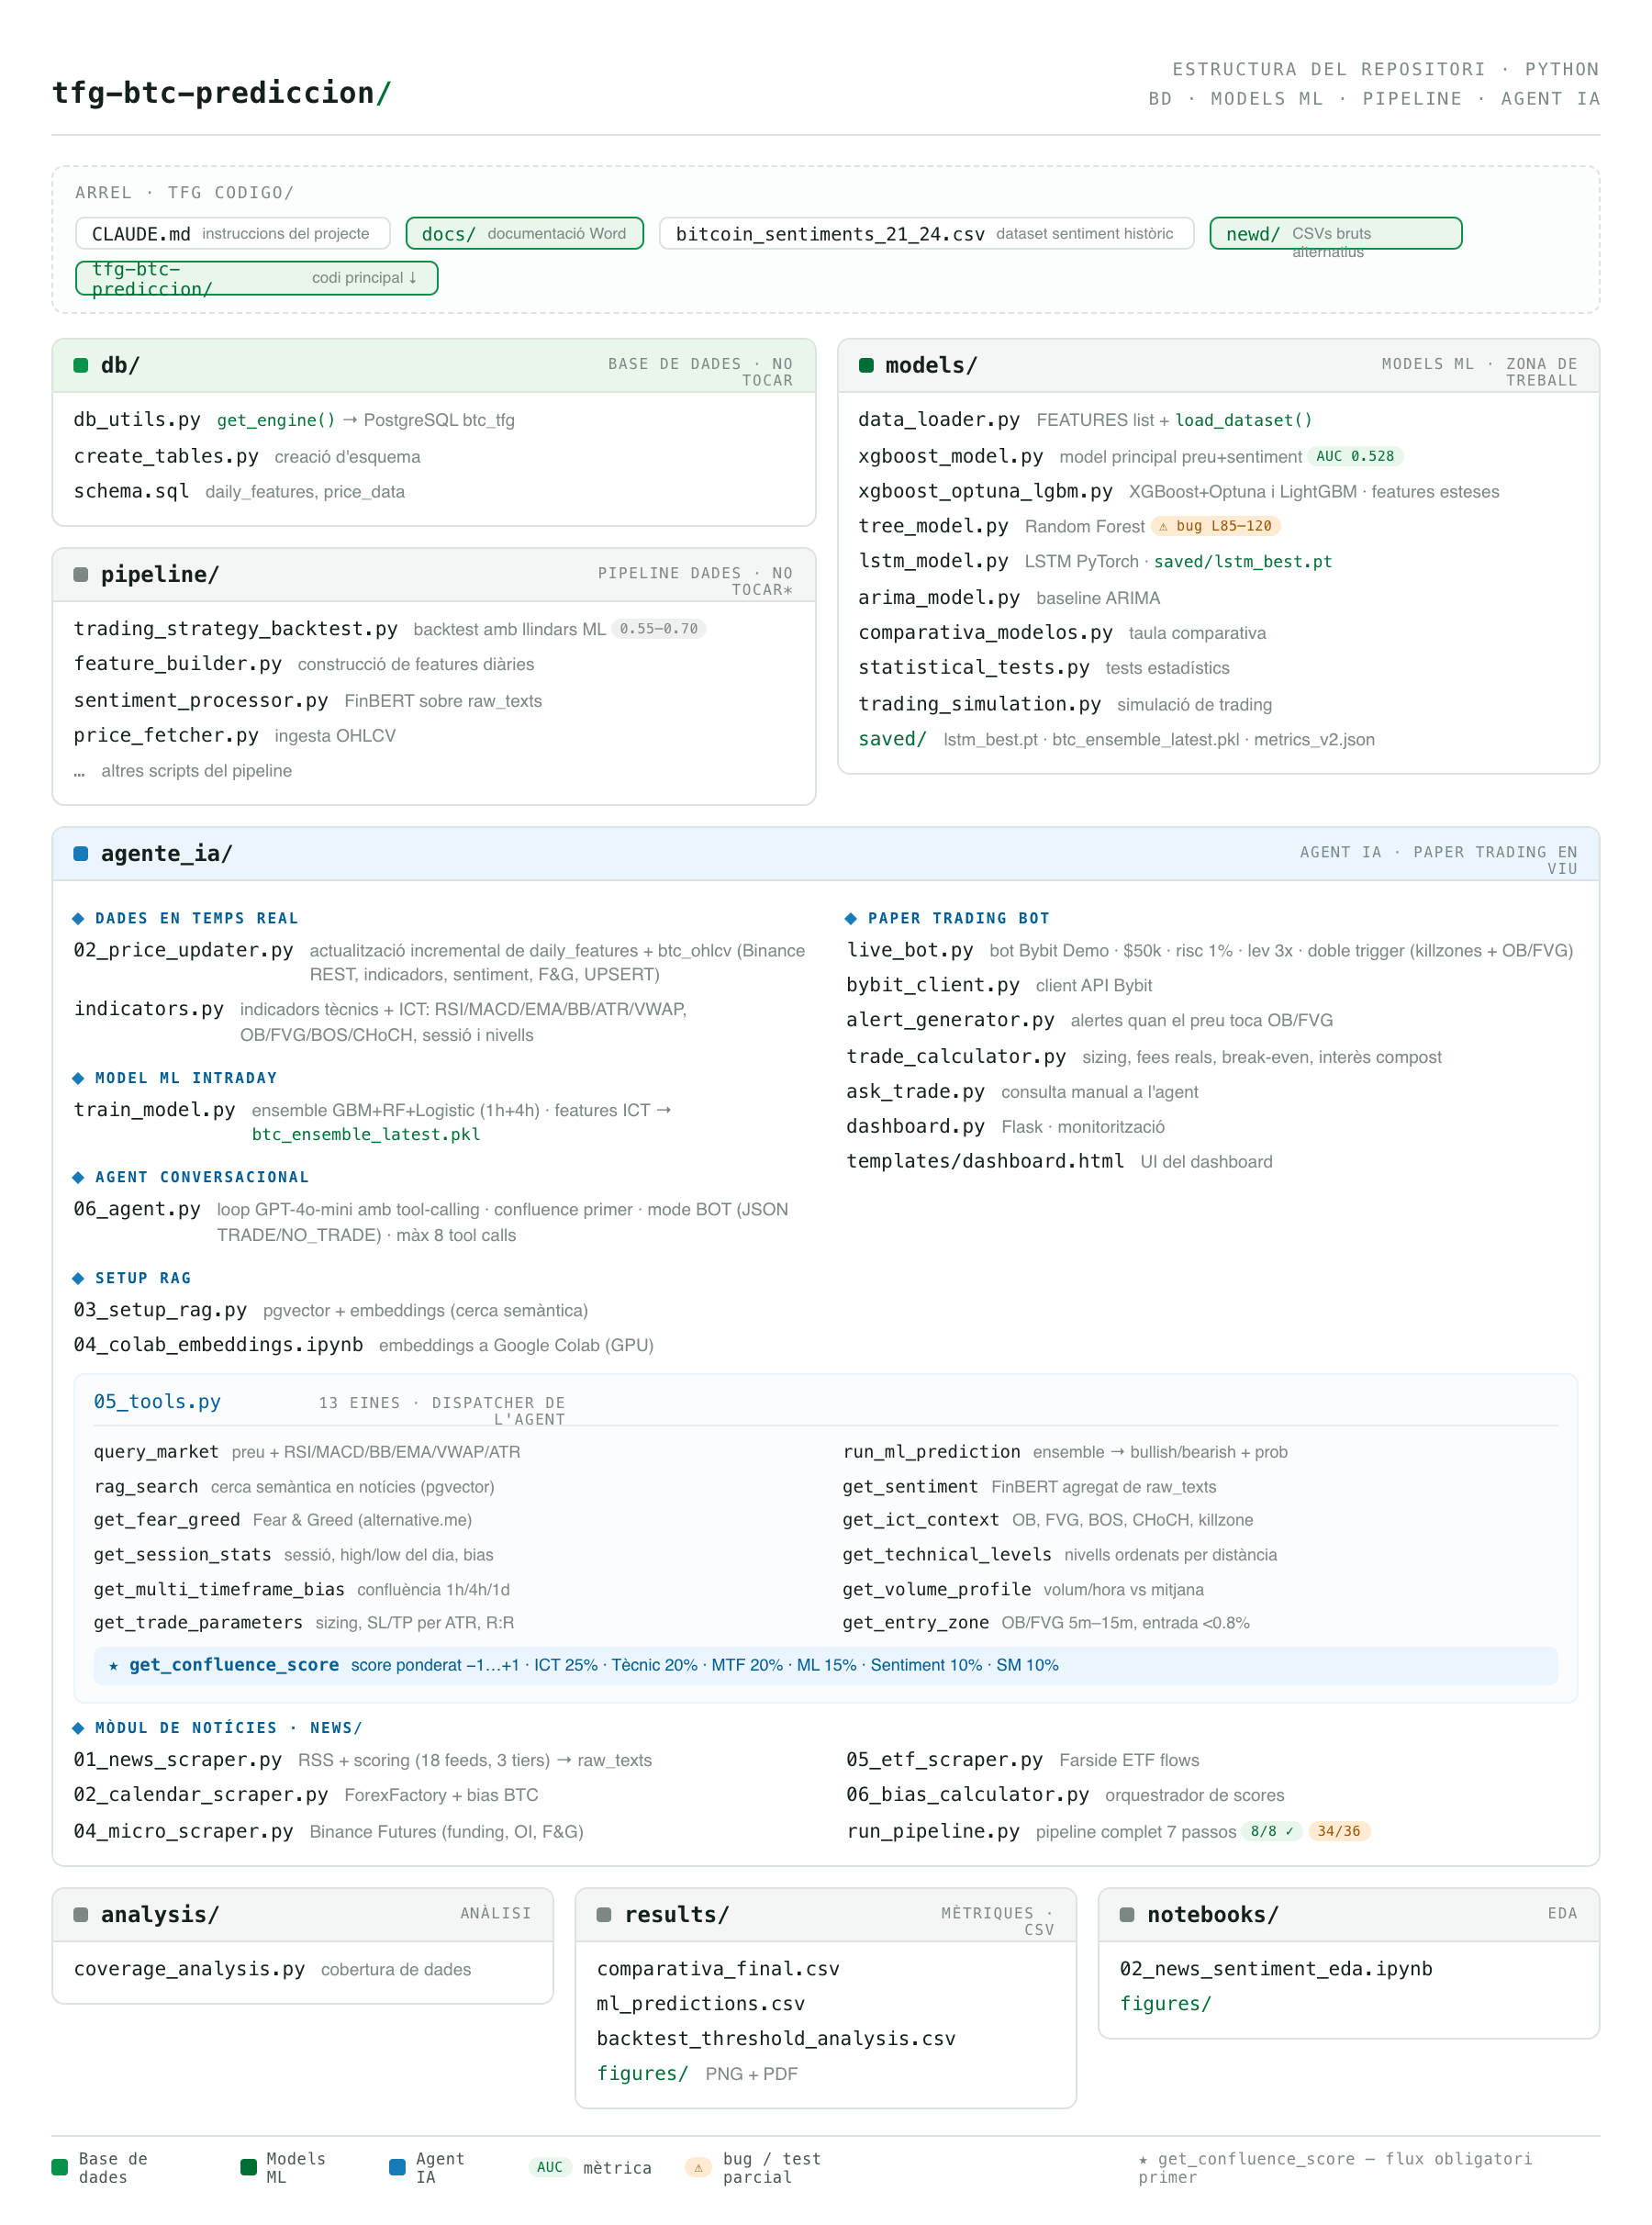
\includegraphics[width=\textwidth]{Estructura-repo.png}
    \caption{Estructura del repositori del sistema de predicció i trading}
    \label{fig:estructura_repo}
\end{figure}

\section{Components principals}

\subsection{Pipeline automàtic diari}

El sistema s'actualitza cada dia sense intervenció manual mitjançant APScheduler a les 00:10 UTC. El pipeline executa sis passos en ordre seqüencial:

\begin{enumerate}
  \item \texttt{price\_fetcher.py} --- descàrrega OHLCV des de Binance API
  \item \texttt{rss\_fetcher.py} --- descàrrega titulars de les 27 fonts RSS
  \item \texttt{fear\_greed\_fetcher.py} --- actualitza el Fear \& Greed Index
  \item \texttt{sentiment\_processor.py} --- processa textos nous amb FinBERT
  \item \texttt{feature\_builder.py} --- recalcula \texttt{daily\_features}
  \item \texttt{logger.py} --- registra resultat, errors i temps
\end{enumerate}

Totes les insercions usen \texttt{ON CONFLICT DO NOTHING} per garantir idempotència.

% ------------------------------------------------------------
%  CAPÍTOL 7 — RECOLECCIÓ DE DADES
% ------------------------------------------------------------
\chapter{Recol\textperiodcentered{}lecció de Dades}

\section{Dades de preu --- Binance API}

Les dades de preu històric s'obtenen de l'API pública de Binance per al parell BTC/USDT en quatre \textit{timeframes}: diari (1d), horari (1h), cada quatre hores (4h) i cada 15 minuts (15m). El volum total actual és de 65.466 registres, cobrint des de l'1 de gener de 2019 fins avui. El Fear \& Greed Index s'obté de l'API d'alternative.me, amb dades històriques des de febrer de 2018.

\section{Corpus de notícies --- procés de construcció}

L'obtenció del corpus de notícies va ser l'aspecte tècnicament més complex del projecte. A continuació es documenta el procés complet, incloent les cinc fonts explorades i descartades.

\subsection{Fonts descartades}

\begin{itemize}
  \item \textbf{Reddit PRAW:} Requereix aprovació manual. La sol\textperiodcentered{}licitud es va realitzar però no va arribar en el termini disponible. El pla gratuït limita l'historial a 1.000 posts per subreddit.

  \item \textbf{CryptoPanic API:} Es va detectar un error de configuració al \texttt{config/.env} on la clau API tenia el prefix duplicat. Una vegada corregit, el pla gratuït només retorna notícies recents.

  \item \textbf{GDELT API directa:} \textit{Rate limiting} molt agressiu (errors 429), amb límit d'1 petició cada 5 segons. Per descarregar el volum necessari haurien calgut més de 20 minuts amb alta probabilitat d'interrupcions.

  \item \textbf{GDELT via BigQuery (primer intent):} Múltiples incompatibilitats en l'esquema de la taula (\texttt{gdeltv2.gkg}) van fer que l'extracció de titulars resultés excessivament complexa. Es va descartar en favor d'una ingestió per \textit{batch} posterior amb esquema simplificat.

  \item \textbf{NewsAPI:} El pla gratuït limita l'historial a un mes enrere.
\end{itemize}

\subsection{Solució adoptada --- corpus de tres components}

\begin{table}[H]
\centering
\caption{Composició del corpus final de notícies (105.125 textos)}
\label{tab:corpus}
\begin{tabular}{@{}L{4.5cm}R{1.8cm}L{3cm}L{3.5cm}@{}}
\toprule
\textbf{Font} & \textbf{Articles} & \textbf{Període} & \textbf{Processament} \\
\midrule
kaggle\_btc\_news\_sentiments & 40.820 & 2011-06 $\to$ 2024-03 & kaggle\_precomputed \\
news\_csv\_2025              & 32.220 & 2025-07 $\to$ 2025-11 & FinBERT \\
kaggle\_btc\_2021\_2024      & 10.081 & 2021-11 $\to$ 2024-09 & kaggle\_precomputed \\
GDELT BigQuery 2025          &  9.325 & 2025-01 $\to$ 2025-12 & FinBERT \\
GDELT BigQuery 2024          &  7.791 & 2024-05 $\to$ 2025-01 & FinBERT \\
GDELT BigQuery 2026          &  2.303 & 2026-01 $\to$ 2026-03 & FinBERT \\
RSS feeds (27 fonts)         & $\approx$1.500 & 2025--2026 & FinBERT \\
Altres fonts                 & $\approx$1.085 & Recents   & FinBERT \\
\midrule
\textbf{TOTAL}               & \textbf{105.125} & \textbf{2011 $\to$ 2026} & \\
\bottomrule
\end{tabular}
\end{table}

Les 27 fonts RSS actives inclouen: CoinDesk (tier~1), Yahoo Finance BTC (tier~1), CoinTelegraph (tier~2), Decrypt (tier~2), The Block (tier~2), GNews BTC (tier~2), AMBCrypto (tier~3), BeInCrypto (tier~3), NewsbtC (tier~3), Bitcoinist (tier~3) i 17 fonts addicionals. La Figura~\ref{fig:cobertura_fonts} resumeix la distribució del corpus per font i per any.

\begin{figure}[H]
\centering
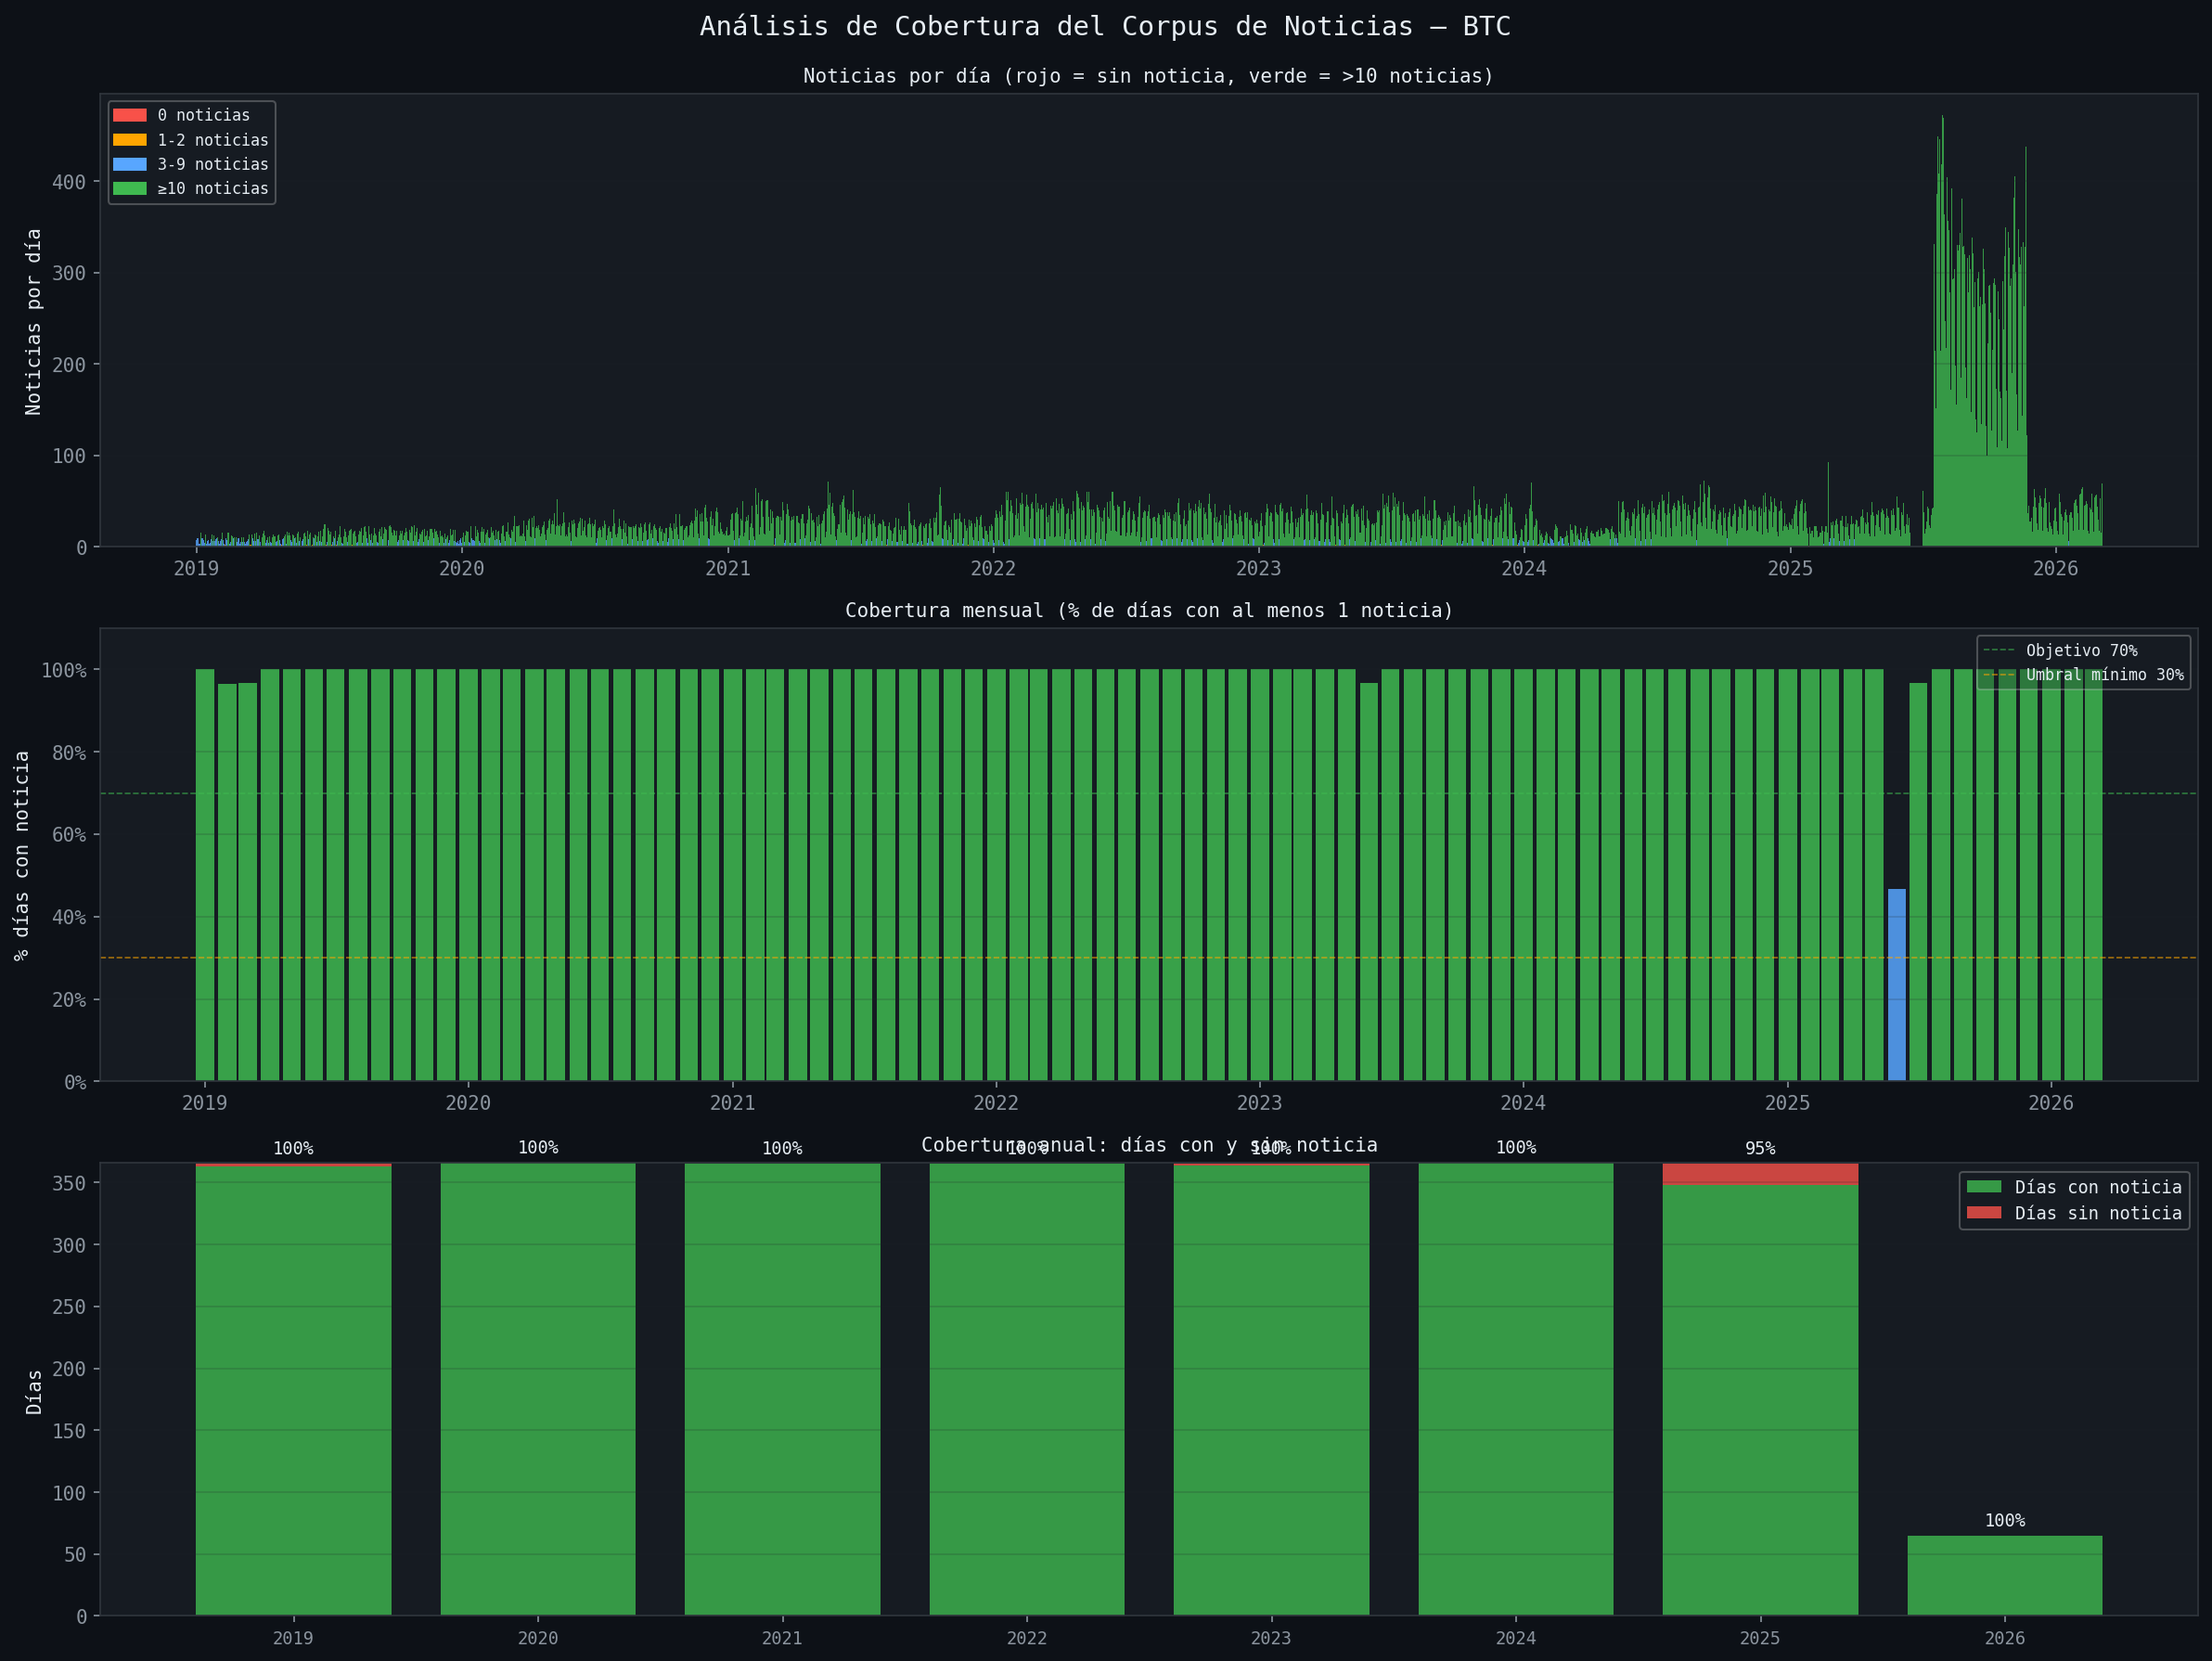
\includegraphics[width=\textwidth]{08_coverage_analysis.png}
\caption{Distribució dels 105.125 articles del corpus per font i per any. Les sis fonts principals aporten el 97,5\% del corpus. La cobertura és del 96,2\% dels dies del dataset ML (2.607 de 2.711 dies amb almenys un article processat amb FinBERT).}
\label{fig:cobertura_fonts}
\end{figure}

\section{Dades per a l'agent d'IA}

El pipeline de notícies de l'agent (\texttt{agente\_ia/news/run\_pipeline.py}) executa 7 passos seqüencials per proporcionar al LLM context suficient:

\begin{enumerate}
  \item \texttt{01\_news\_scraper.py} --- 27 fonts RSS amb \textit{scoring} de decaïment temporal
  \item \texttt{02\_calendar\_scraper.py} --- Calendari macroeconòmic (Fed, CPI, NFP)
  \item \texttt{03\_onchain\_scraper.py} --- Mètriques \textit{on-chain} de CryptoQuant
  \item \texttt{04\_micro\_scraper.py} --- \textit{Funding rate}, \textit{open interest}, liquidacions
  \item \texttt{05\_etf\_scraper.py} --- Fluxos nets diaris ETFs spot BTC (IBIT, FBTC, ARKB\ldots)
  \item \texttt{06\_bias\_calculator.py} --- \textit{Snapshot} de biaix multi-modal
  \item \texttt{run\_pipeline.py} --- Orquestrador: genera el context comprimit pel LLM
\end{enumerate}

\subsection{Per què les dades macroeconòmiques i de microestructura són clau}

Aquests mòduls van més enllà del simple \textit{scraping} de notícies. La integració de fonts heterogènies respon a una limitació fonamental de les senyals de sentiment: la seva incapacitat per capturar el context estructural del mercat.

\textbf{Calendari macroeconòmic (02):} Esdeveniments com les reunions de la Reserva Federal (Fed), la publicació del CPI (\textit{Consumer Price Index}, la mesura d'inflació dels EUA) o les dades del NFP (\textit{Non-Farm Payrolls}, indicador d'ocupació) tenen un impacte mesurable i sistemàtic sobre Bitcoin. Quan la Fed puja els tipus d'interès, el capital tendeix a sortir d'actius d'alt risc com BTC cap a renda fixa. El model de sentiment no pot saber si avui hi ha una reunió del FOMC; el calendari macroeconòmic sí.

\textbf{Microestructura del mercat (04):} El \textit{funding rate} dels futurs perpetuos és probablement la senyal de microestructura més valuosa. Quan el \textit{funding rate} és molt positiu, els llargs (\textit{longs}) paguen als curts (\textit{shorts}), indicant que el mercat està molt apalancat en pujada i és vulnerable a una correcció (squeeze). L'\textit{open interest} mesura el volum total de posicions obertes; un OI creixent amb preu creixent és una senyal de tendència; un OI decreixent amb preu creixent pot indicar que la pujada és feble.

\textbf{Fluxos ETF (05):} Des de l'aprovació dels ETFs spot de Bitcoin als EUA el gener de 2024, els fluxos nets diaris d'instruments com l'IBIT de BlackRock o el FBTC de Fidelity han esdevingut senyals d'adopció institucional amb impacte directe en el preu. Un dia amb entrades de 500M\$ als ETFs spot és qualitativament diferent d'un dia amb sortides, i aquesta informació no apareix als titulars de les notícies de criptomonedes.

\textbf{On-chain (03):} Mètriques com el SOPR (\textit{Spent Output Profit Ratio}), que mesura si els \textit{outputs} de transaccions de Bitcoin s'estan movent en guanys o en pèrdues, o els \textit{exchange inflows} (quantitat de BTC que entra als \textit{exchanges}, sovint preludi de venda), aporten una perspectiva que els indicadors tècnics basats en OHLCV no capturen.

El \textit{bias calculator} (06) combina totes aquestes senyals en un únic indicador de biaix direccional que el LLM pot interpretar directament, sense haver de raonar sobre cada font de forma independent.

% ------------------------------------------------------------
%  CAPÍTOL 8 — EMMAGATZEMATGE DE DADES
% ------------------------------------------------------------
\chapter{Emmagatzematge de Dades}

\section{Disseny de l'esquema}

La base de dades \texttt{btc\_tfg} a PostgreSQL~15 conté 12 taules organitzades en tres dominis funcionals:

\begin{table}[H]
\centering
\caption{Taules de la base de dades btc\_tfg}
\label{tab:bd}
\begin{tabular}{@{}llrr@{}}
\toprule
\textbf{Taula} & \textbf{Descripció} & \textbf{Files} & \textbf{Mida} \\
\midrule
\multicolumn{4}{l}{\textit{Domini preu}} \\
price\_data           & OHLCV diari i intraday BTC (Binance)    & 65.466  & 12~MB \\
hourly\_features      & Features horàries per a l'agent IA      & 62.814  & 18~MB \\
btc\_ohlcv            & OHLCV intraday consolidat (15m-1d)      &  5.374  & 4.5~MB \\
\midrule
\multicolumn{4}{l}{\textit{Domini text i sentiment}} \\
raw\_texts            & Corpus de notícies (45 fonts totals: 27 RSS + datasets)           & 105.125 & 58~MB \\
sentiment\_scores     & Scores FinBERT per article              & 103.002 & 15~MB \\
daily\_features       & Taula mestra ML (target + features)     &   2.711 & 1.5~MB \\
\midrule
\multicolumn{4}{l}{\textit{Domini context de l'agent}} \\
economic\_calendar    & Esdeveniments macro programats          &     783 & 480~KB \\
institutional\_flows  & Fluxos ETF spot BTC diaris              &     286 & 200~KB \\
market\_microstructure& Funding rate, OI, liquidacions          &     330 & 144~KB \\
on\_chain\_metrics    & Exchange inflows, SOPR, MVRV            &      12 & 88~KB \\
bias\_snapshots       & Snapshots biaix multi-modal             &       9 & 64~KB \\
live\_trades          & Operacions del \textit{paper trading} bot &      1 & 80~KB \\
\bottomrule
\end{tabular}
\end{table}

\vspace{8cm}
\section{Esquema de la taula diària principal}

La Figura~\ref{fig:esquema_bd} mostra l'esquema relacional complet de la base de dades del pipeline ML.

\begin{figure}[H]
    \centering
    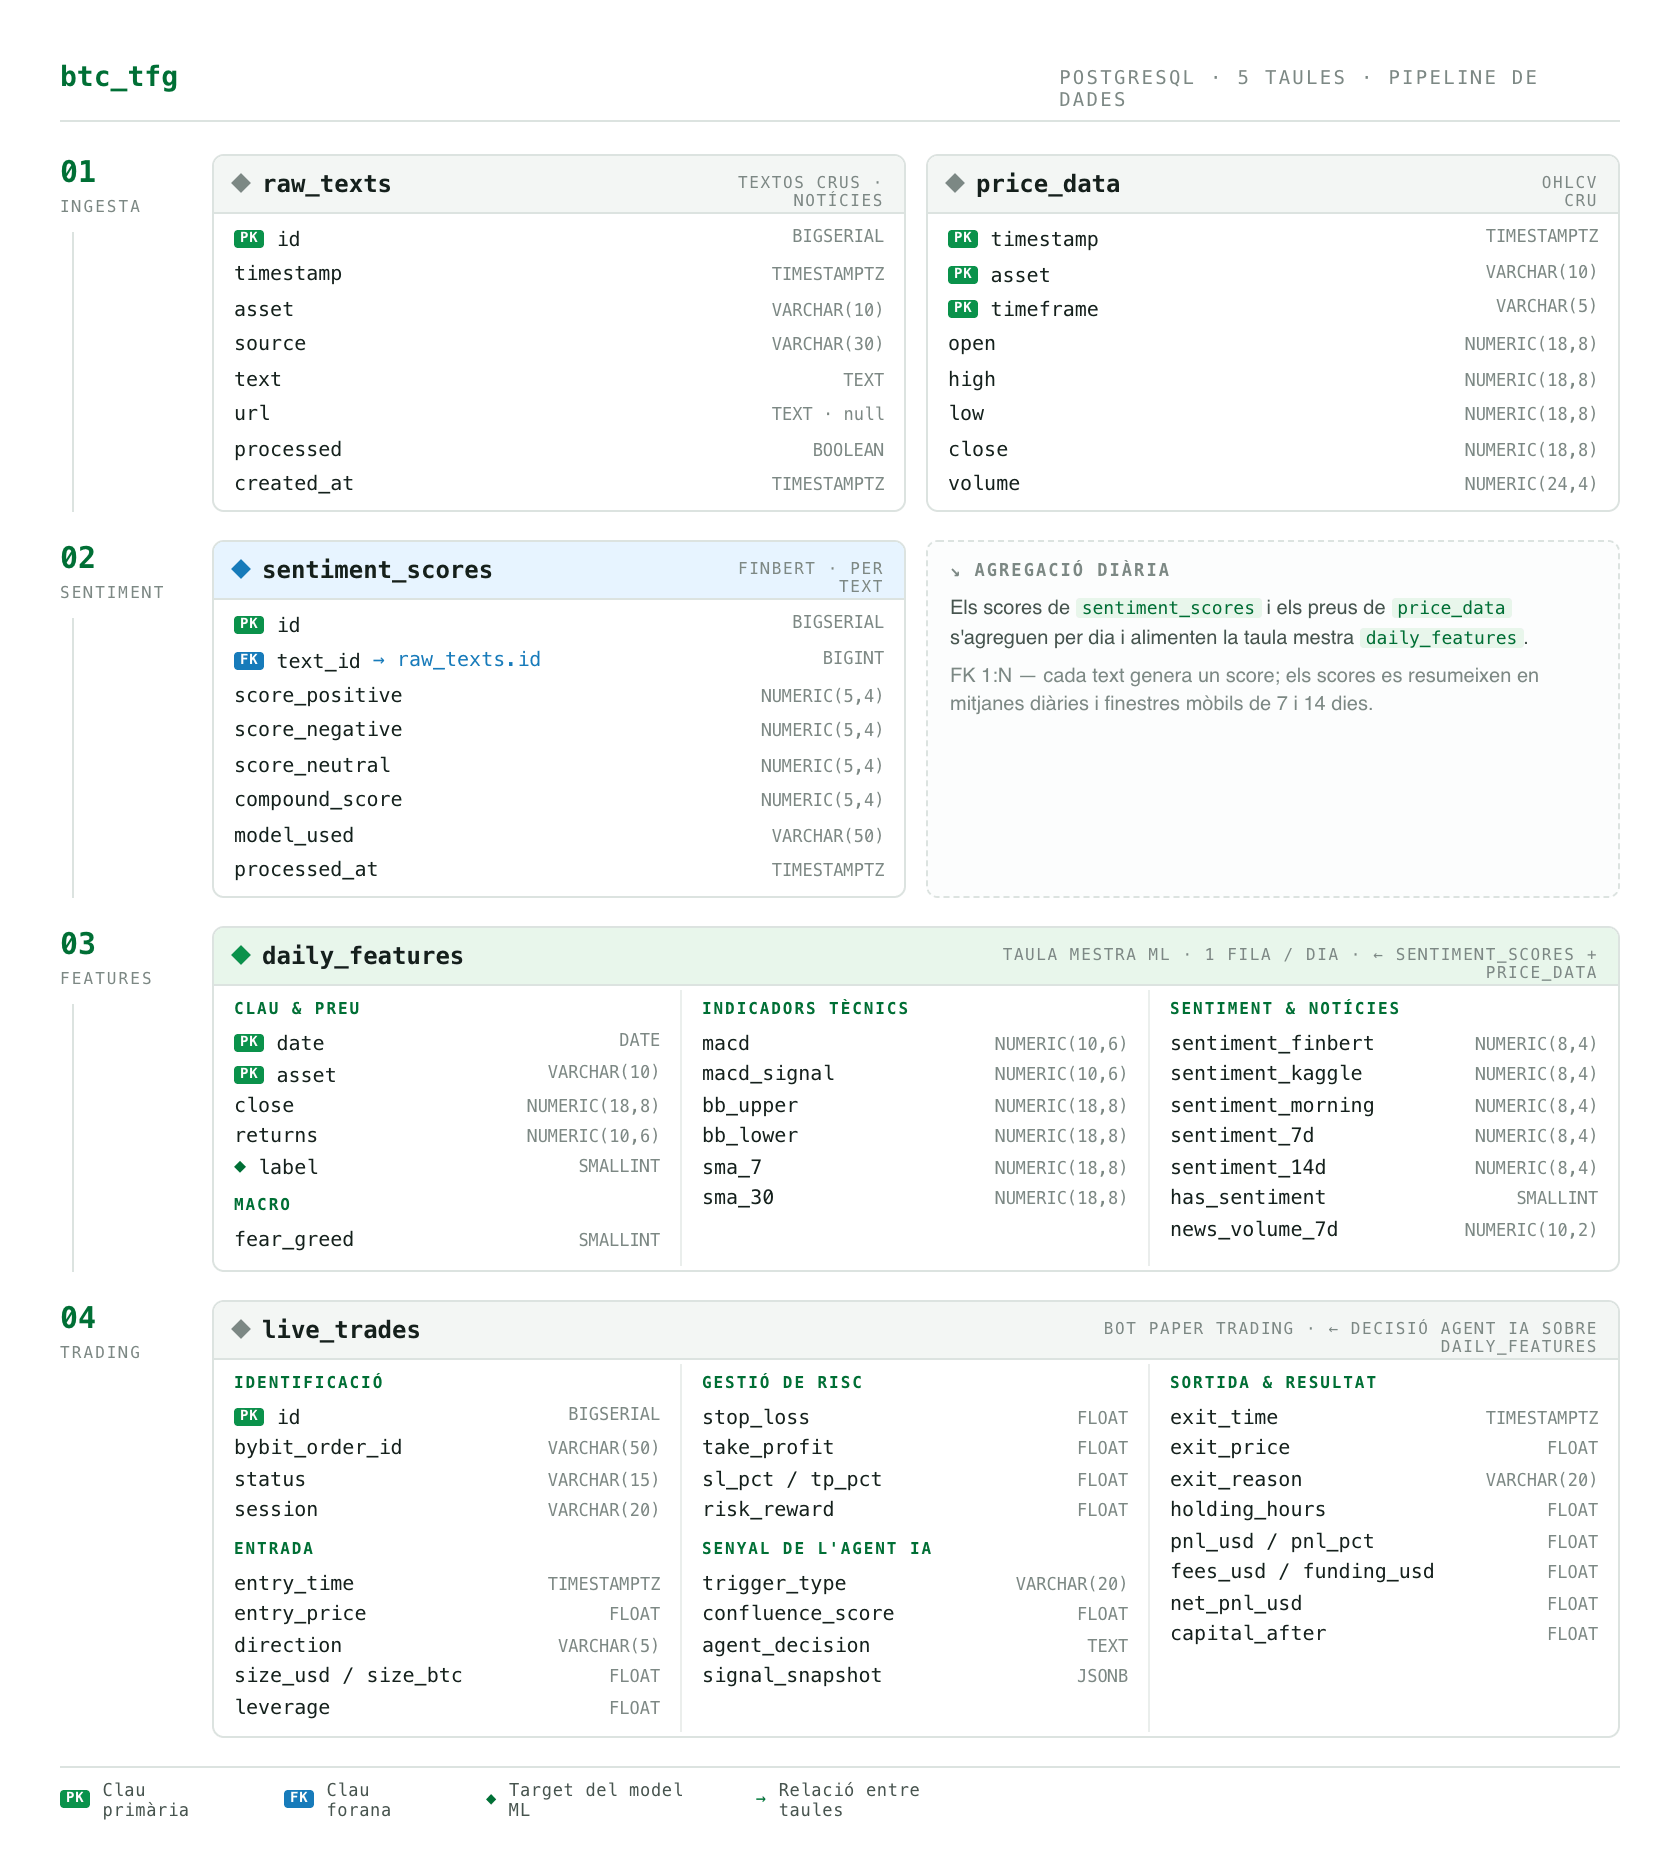
\includegraphics[width=\textwidth]{Esquema-BD.png}
    \caption{Esquema de la base de dades del pipeline ML}
    \label{fig:esquema_bd}
\end{figure}

\section{Decisions de disseny}

\textbf{PostgreSQL vs SQLite:} Es va elegir PostgreSQL pel seu suport natiu de timestamps amb zona horària (TIMESTAMPTZ, essencial per a dades financeres multi-exchange), l'escalabilitat a connexions concurrents i un ecosistema d'extensions ric. La cerca semàntica es va acabar resolent amb FAISS (vegeu Capítol~\ref{cap:agent}).

\textbf{Separació de models de sentiment:} Un problema crític detectat a l'auditoria va ser la mescla de \textit{scores} de dos models amb distribucions incompatibles (FinBERT continu, mitjana +0.052; Kaggle discret, mitjana $-0.282$). La solució va ser afegir la columna \texttt{model\_used} i calcular columnes separades a \texttt{daily\_features}.

% ------------------------------------------------------------
%  CAPÍTOL 9 — PROCESSAMENT I ANÀLISI DE DADES
% ------------------------------------------------------------
\chapter{Processament i Anàlisi de Dades}

\section{Feature engineering}

El mòdul \texttt{feature\_builder.py} calcula diàriament les transformacions següents:

\begin{itemize}
  \item \textbf{Retorn logarítmic:} $r_t = \ln(\mathrm{Close}_t / \mathrm{Close}_{t-1})$
  \item \textbf{RSI-14:} Oscil\textperiodcentered{}lador de \textit{momentum} a [0, 100]
  \item \textbf{MACD (12, 26, 9):} Diferència entre EMA-12 i EMA-26
  \item \textbf{Bandes de Bollinger (20, 2$\sigma$):} Canal de volatilitat
  \item \textbf{SMA-7 i SMA-30:} Mitjanes mòbils simples
\end{itemize}

Per al sentiment, es calculen tres versions:

\begin{itemize}
  \item \texttt{sentiment\_finbert}: Mitjana dels \textit{scores} FinBERT de tots els articles del dia $t$
  \item \texttt{sentiment\_morning}: Mitjana dels articles publicats \textbf{abans de les 18:00 UTC} del dia $t$ (per a l'experiment de causalitat inversa)
  \item \texttt{has\_sentiment}: \textit{Flag} binari que indica si hi ha dades FinBERT disponibles
\end{itemize}

\section{Anàlisi Exploratòria (EDA)}

L'EDA sobre 2.711 observacions diàries (2019-01-01 a 2026-06-03) va produir les troballes següents.

% ---- FIG 1: notebooks/figures/01_precio_tecnico_sentiment.png -> fig01_preu_sentiment.png ----
\begin{figure}[H]
\centering
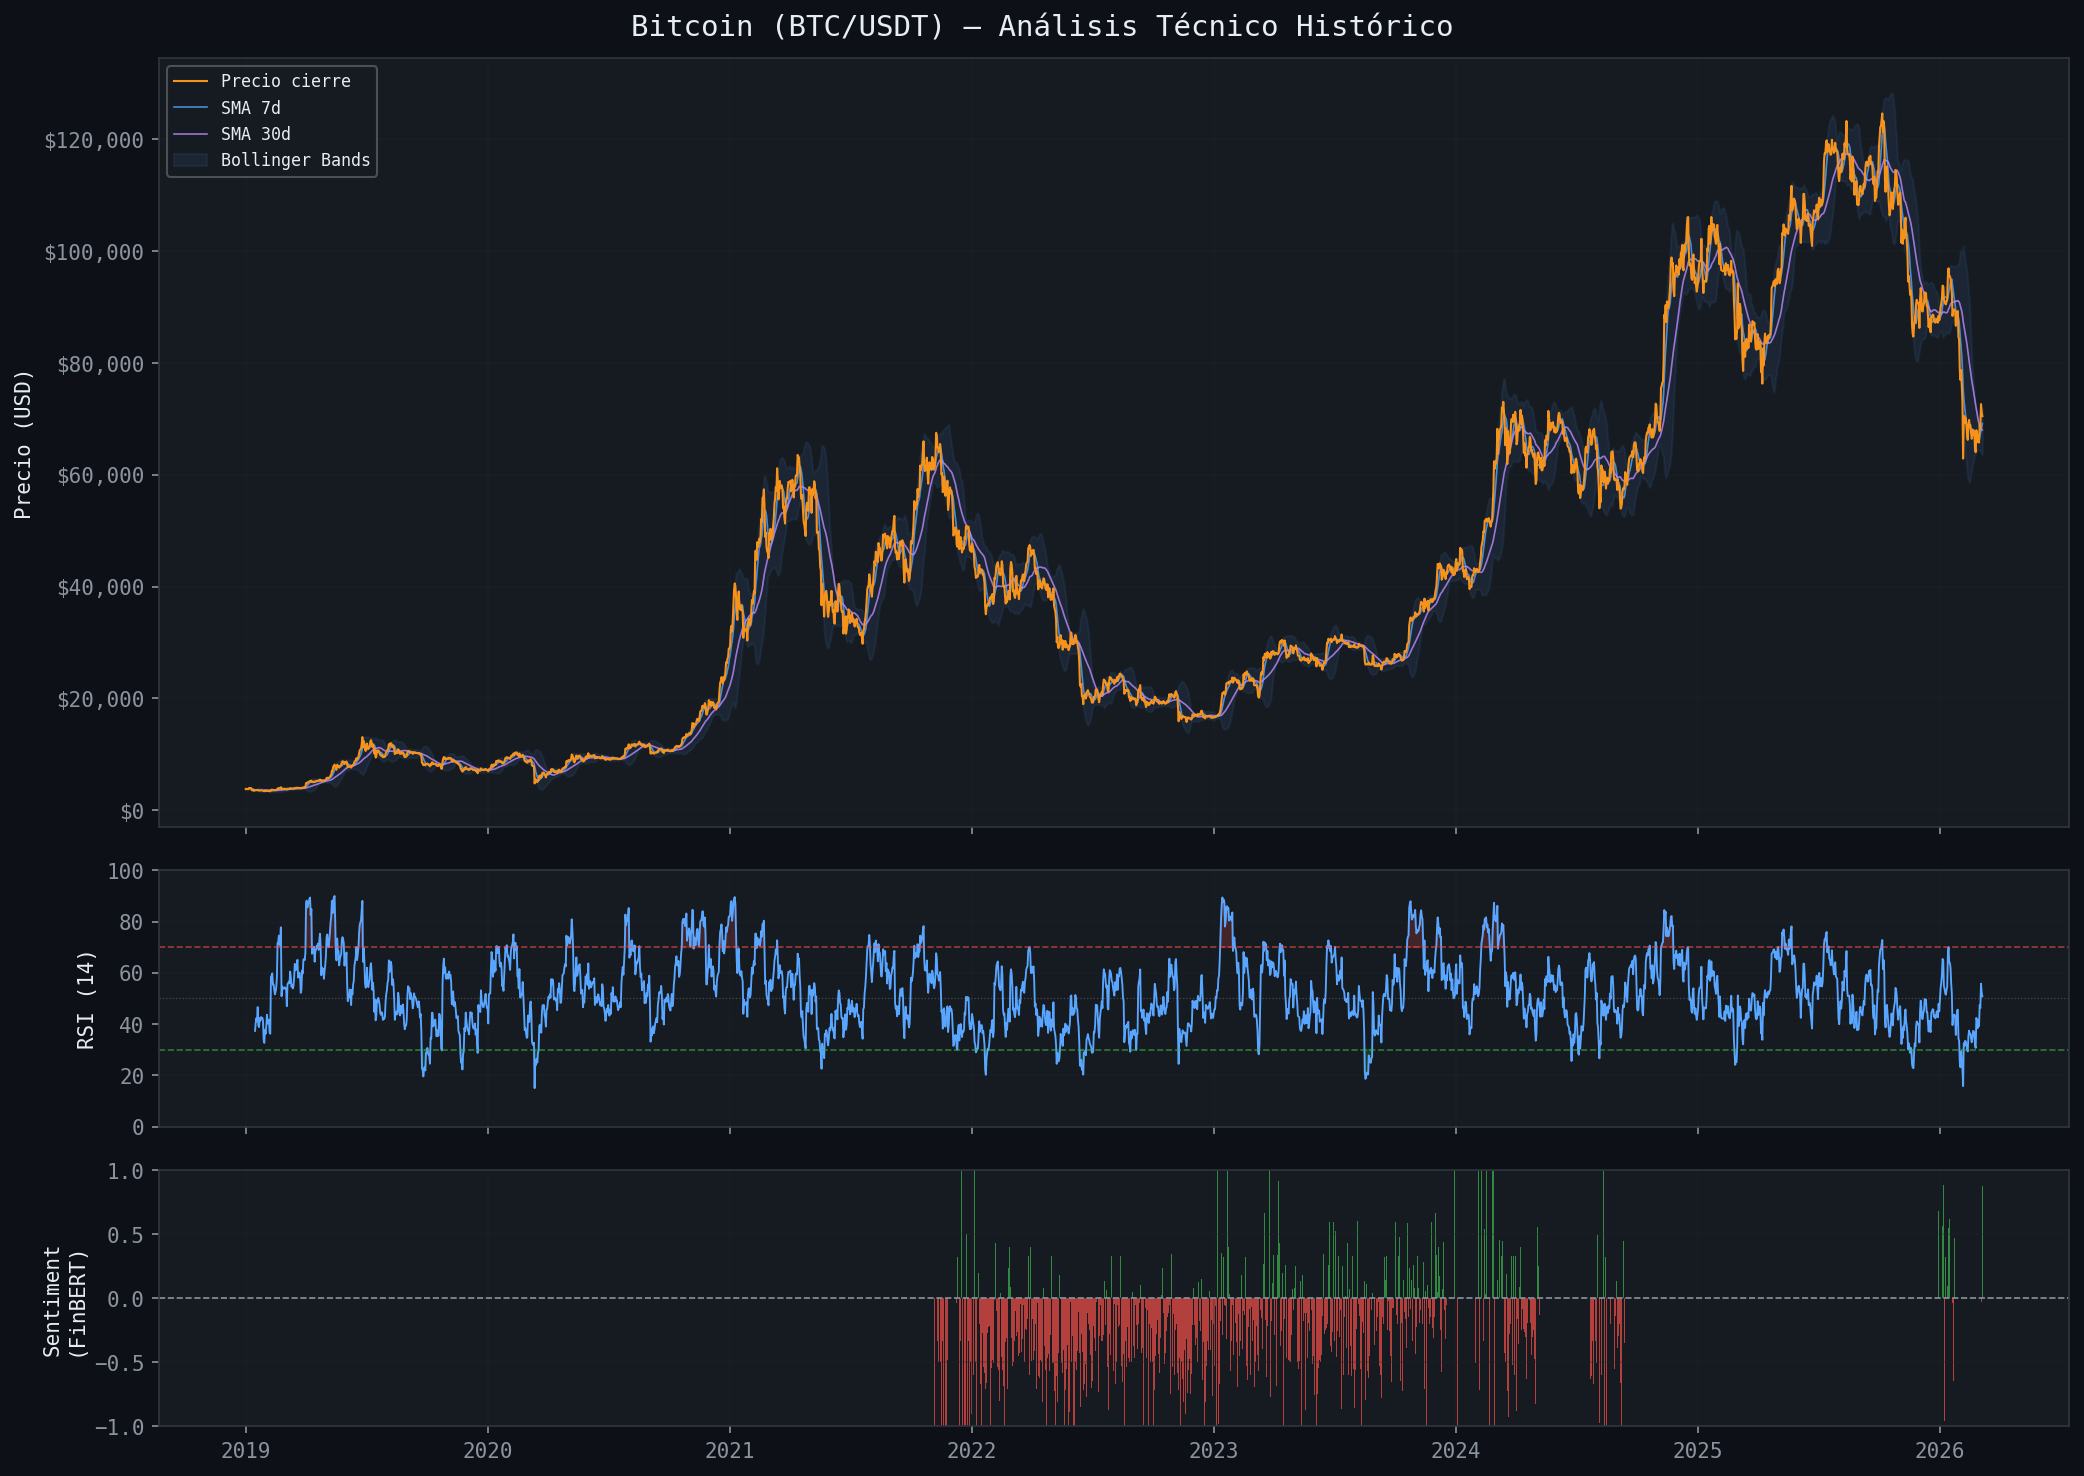
\includegraphics[width=\textwidth]{fig01_preu_sentiment}
\caption{Evolució del preu de BTC/USDT (superior) amb SMA-7, SMA-30 i Bandes de Bollinger; RSI-14 (central) amb llindars de sobrecompra (70) i sobrevenda (30); i sentiment diari FinBERT (inferior), 2019--2026. S'identifiquen els grans cicles: bull run 2020--21, crash FTX novembre 2022 (RSI $< 30$, barres vermelles) i rally 2024. La correlació visual és descriptiva, no predictiva (Mann-Whitney $p = 0.342$).}
\label{fig:preu_sentiment}
\end{figure}

\textbf{Distribució del dataset:} 1.382 dies alcistes (51.0\%) front a 1.329 baixistes (49.0\%). El dataset és pràcticament equilibrat; no cal aplicar tècniques de balanceig de classes.

% ---- FIG 2: notebooks/figures/02_distribucion_label.png -> fig02_distribucio_label.png ----
\begin{figure}[H]
\centering
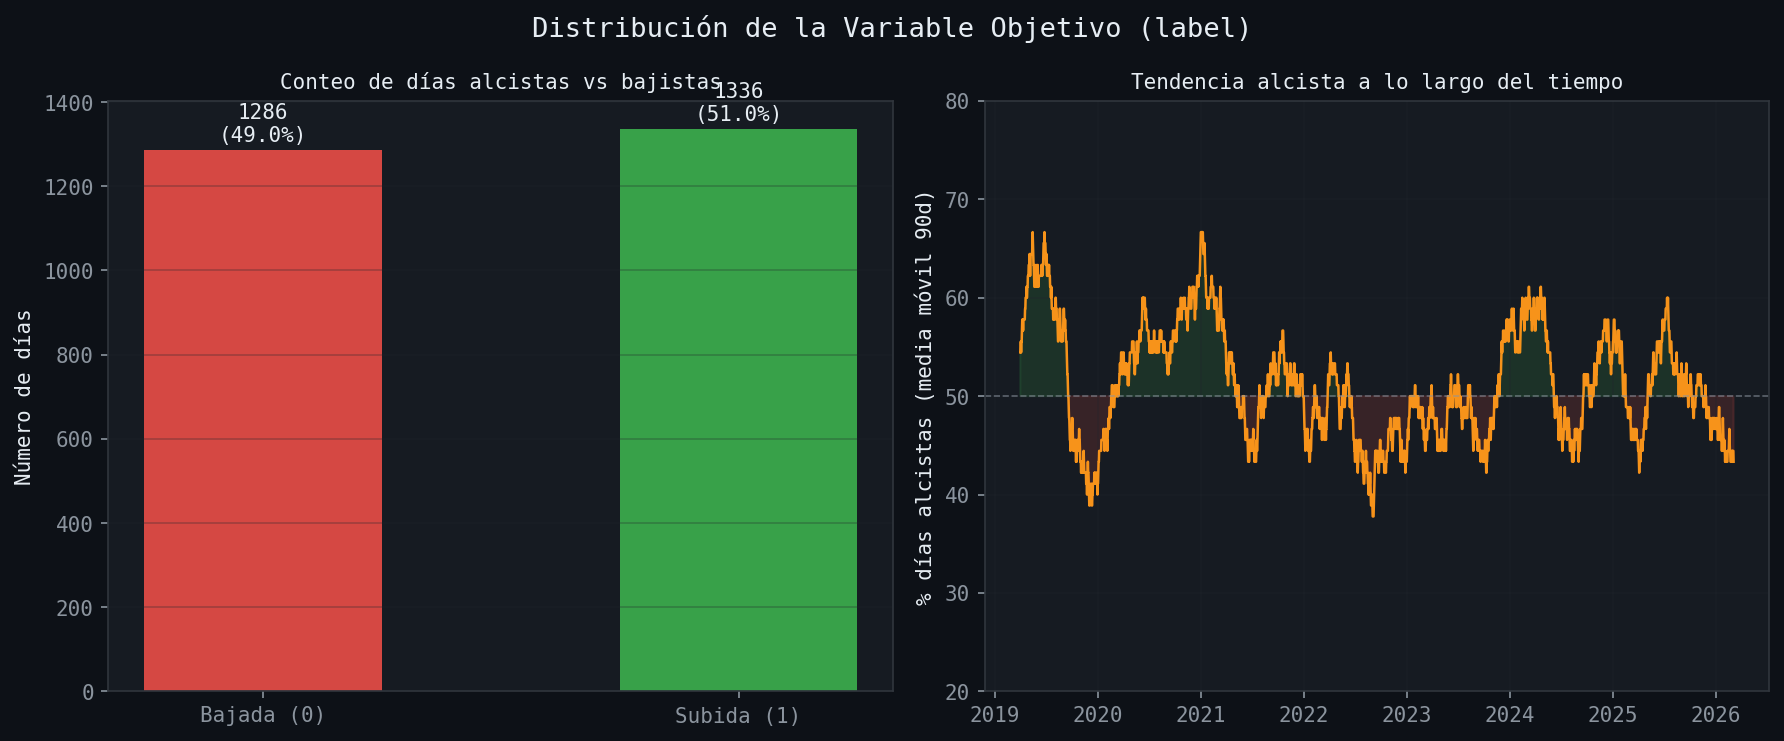
\includegraphics[width=0.9\textwidth]{fig02_distribucio_label}
\caption{Distribució de la variable objectiu. Esquerra: 1.382 dies alcistes (51,0\%) vs 1.329 baixistes (49,0\%). Dreta: percentatge de dies alcistes amb mitjana mòbil de 90 dies. La línia discontínua al 50\% representa el baseline aleatori. El dataset equilibrat confirma que no cal aplicar SMOTE ni \textit{oversampling}.}
\label{fig:distribucio_label}
\end{figure}

\textbf{Correlacions amb l'objectiu:} Totes les correlacions de Pearson són molt febles ($|r| < 0.08$), resultat consistent amb la hipòtesi de mercat eficient. La feature més correlacionada és \texttt{returns} ($r = -0.0725$, reversió a la mitjana).

\begin{table}[H]
\centering
\caption{Correlació de Pearson de cada \textit{feature} amb el \textit{label}}
\label{tab:correlacio}
\begin{tabular}{@{}lr@{}}
\toprule
\textbf{Feature} & \textbf{Correlació} \\
\midrule
returns            & $-0.0725$ \\
bb\_lower          & $-0.0303$ \\
sma\_7             & $-0.0296$ \\
sma\_30            & $-0.0295$ \\
bb\_upper          & $-0.0286$ \\
fear\_greed        & $+0.0246$ \\
sentiment\_morning & $-0.0185$ \\
sentiment\_finbert & $-0.0172$ \\
macd\_signal       & $+0.0165$ \\
macd               & $+0.0063$ \\
rsi\_14            & $-0.0042$ \\
has\_sentiment     & $-0.0028$ \\
\bottomrule
\end{tabular}
\end{table}

% ---- FIG 3: notebooks/figures/03_correlacion_features.png -> fig03_correlacio_features.png ----
\begin{figure}[H]
\centering
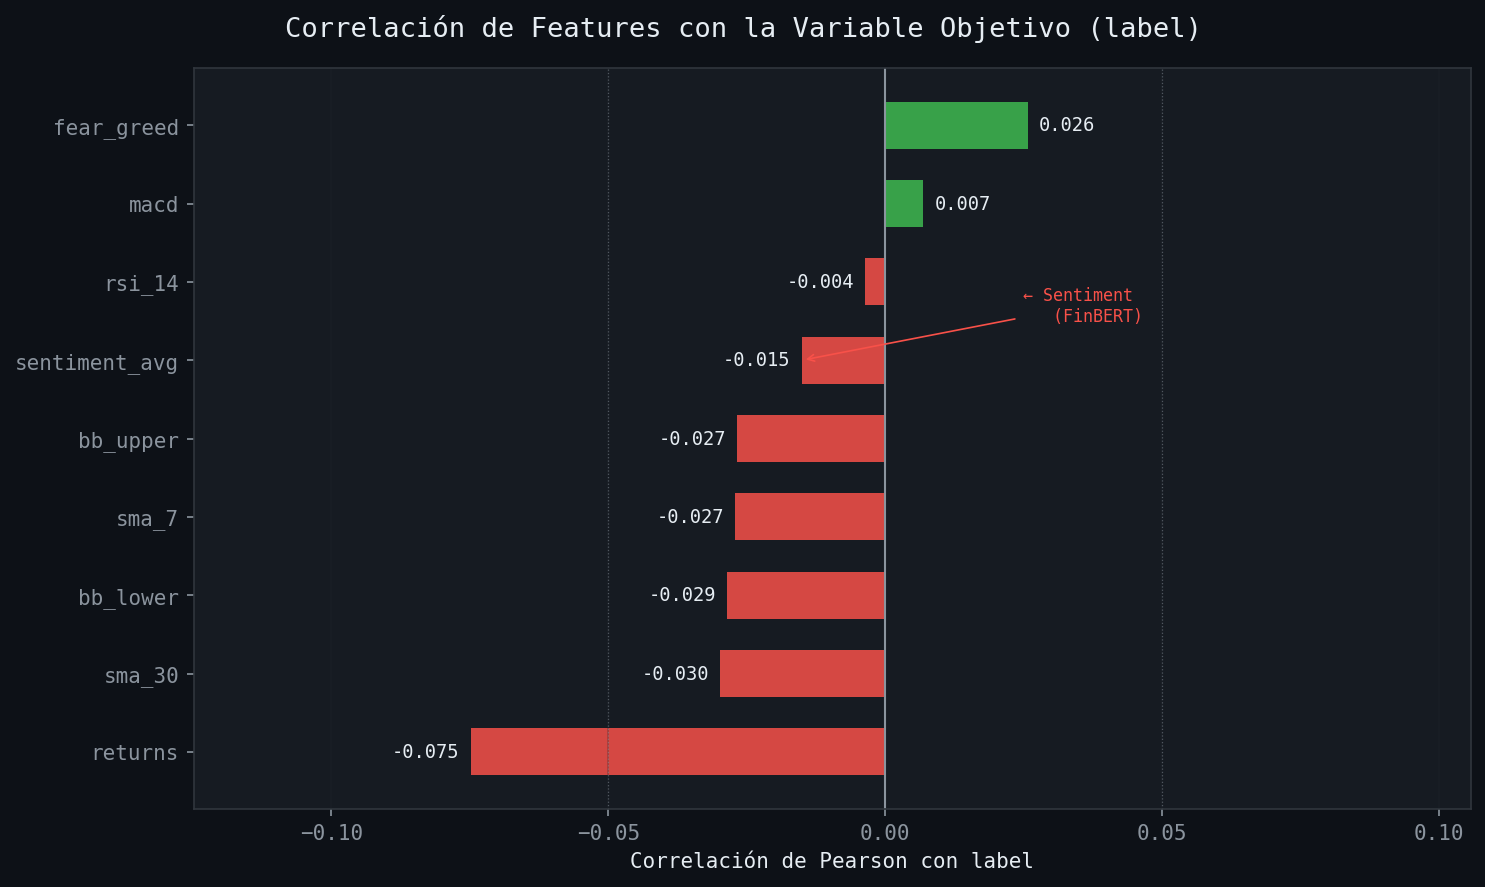
\includegraphics[width=0.85\textwidth]{fig03_correlacio_features}
\caption{Correlació de Pearson de cada feature amb el label (2019--2026). Totes les correlacions estan per sota de $|r| = 0.08$, consistent amb la hipòtesi d'eficiència de mercat. Les barres taronges corresponen a features de sentiment; les blaves, a indicadors tècnics. La baixa correlació lineal no implica inutilitat per als models no lineals com XGBoost, que pot explotar interaccions entre features.}
\label{fig:correlacio_features}
\end{figure}

\textbf{Test Mann-Whitney (alcistes vs baixistes):} $U = 821.316{,}5$, $p = 0.342$. Les distribucions de sentiment en dies alcistes i baixistes són estadísticament indistingibles.

Les Figures~\ref{fig:sentiment_preu} i~\ref{fig:lag_analysis} il\textperiodcentered{}lustren, respectivament, la relació temporal entre sentiment i preu i l'anàlisi de correlació del sentiment amb el label a diferents \textit{lags}.

% ---- FIG 4: notebooks/figures/04_sentiment_vs_precio.png -> fig04_sentiment_preu.png ----
\begin{figure}[H]
\centering
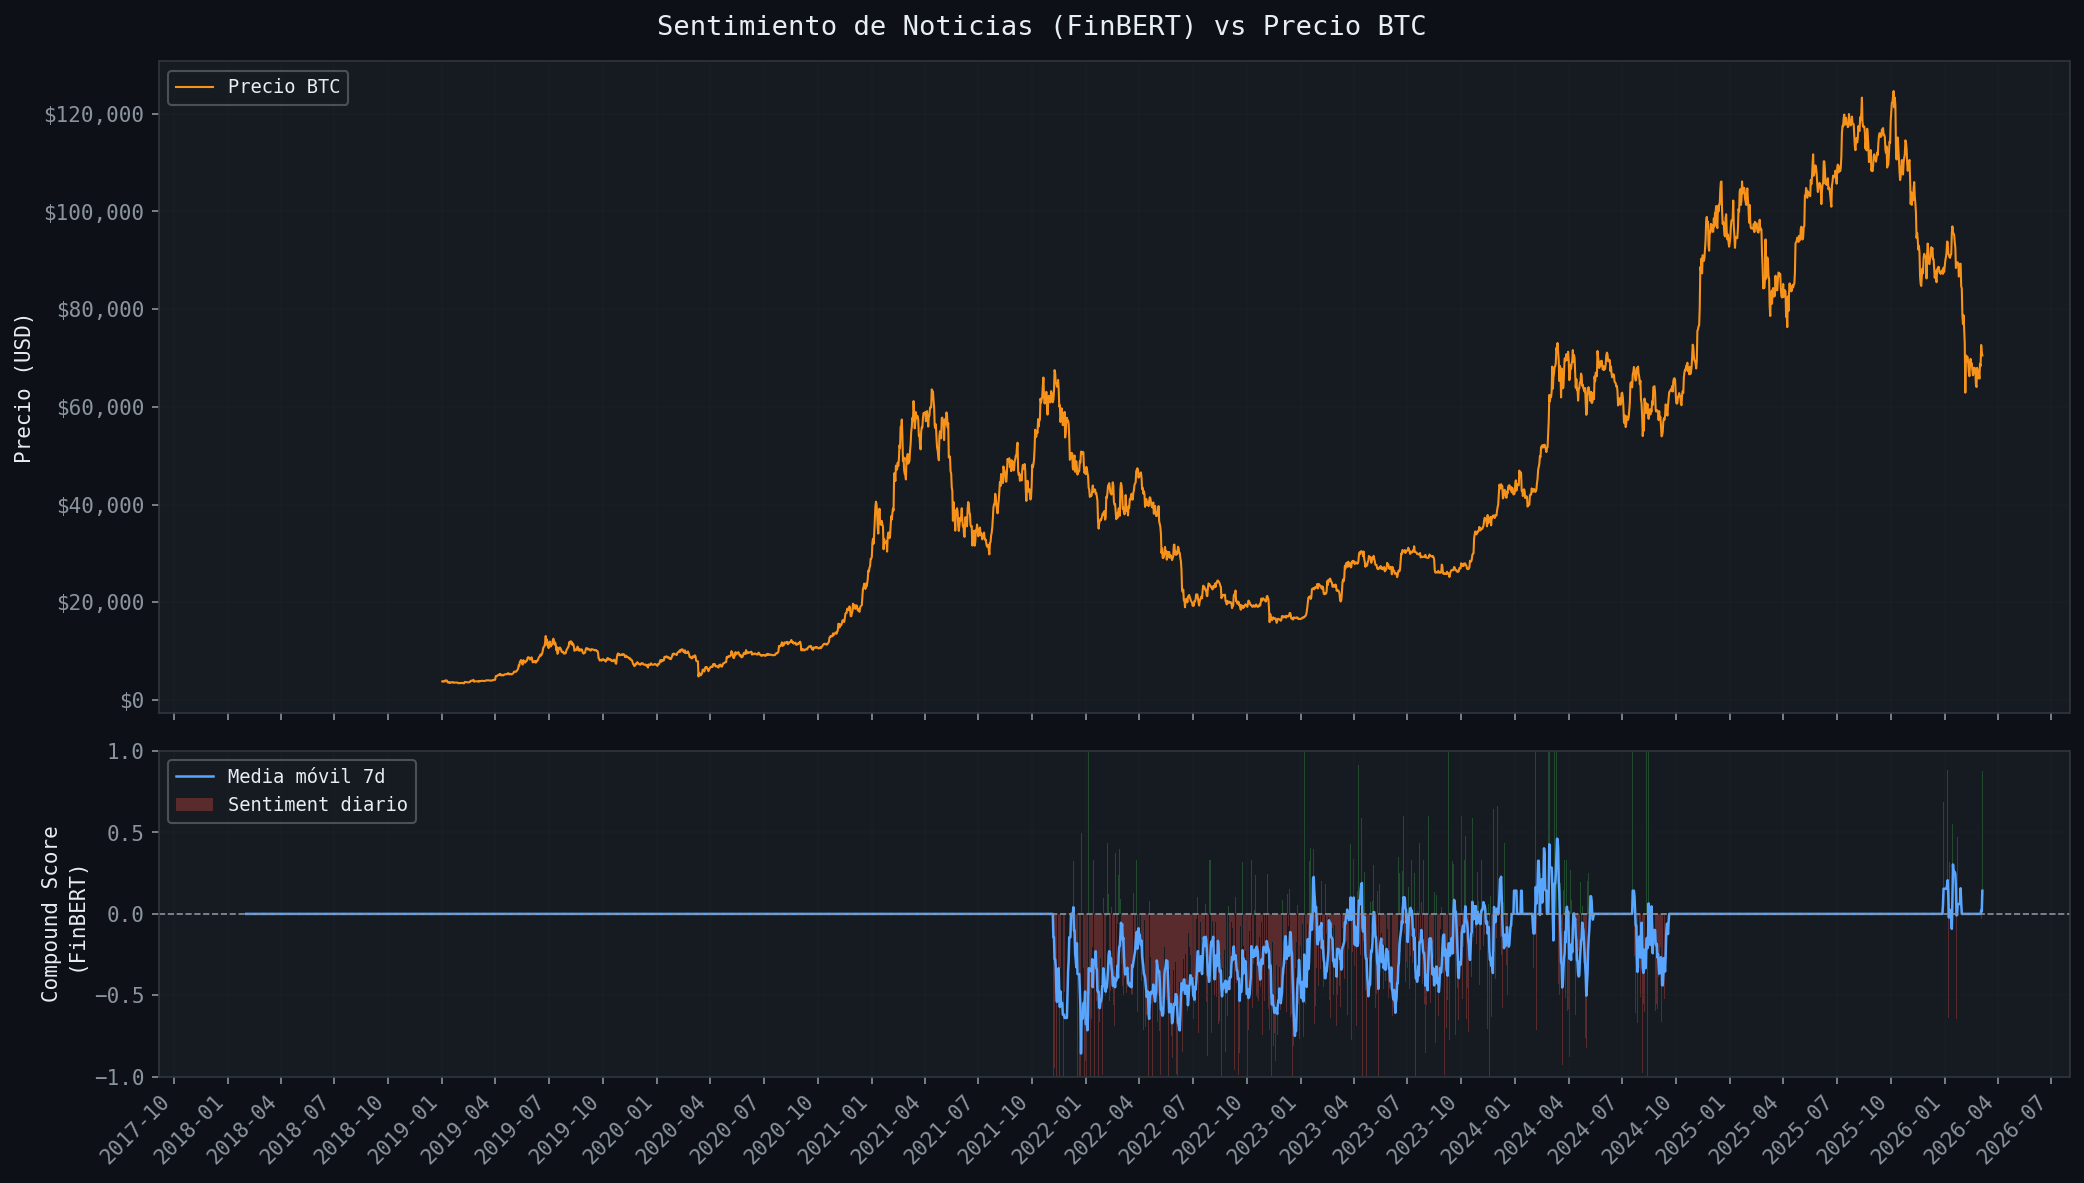
\includegraphics[width=\textwidth]{fig04_sentiment_preu}
\caption{Relació temporal entre el sentiment FinBERT diari (barres) i la seva mitjana mòbil de 7 dies (línia blava) sobre el preu de BTC. Els màxims de preu de 2021 i 2024 van acompanyats de sentiment positiu sostingut; els períodes baixistes presenten barres vermelles més freqüents. Aquesta observació visual justifica la incorporació del sentiment com a feature, tot i que la causalitat és inversa: les notícies descriuen el preu, no l'anticipen.}
\label{fig:sentiment_preu}
\end{figure}

% ---- FIG 11: results/figures/fig11_lag_analysis.png -> fig11_lag_analysis.png ----
\begin{figure}[H]
\centering
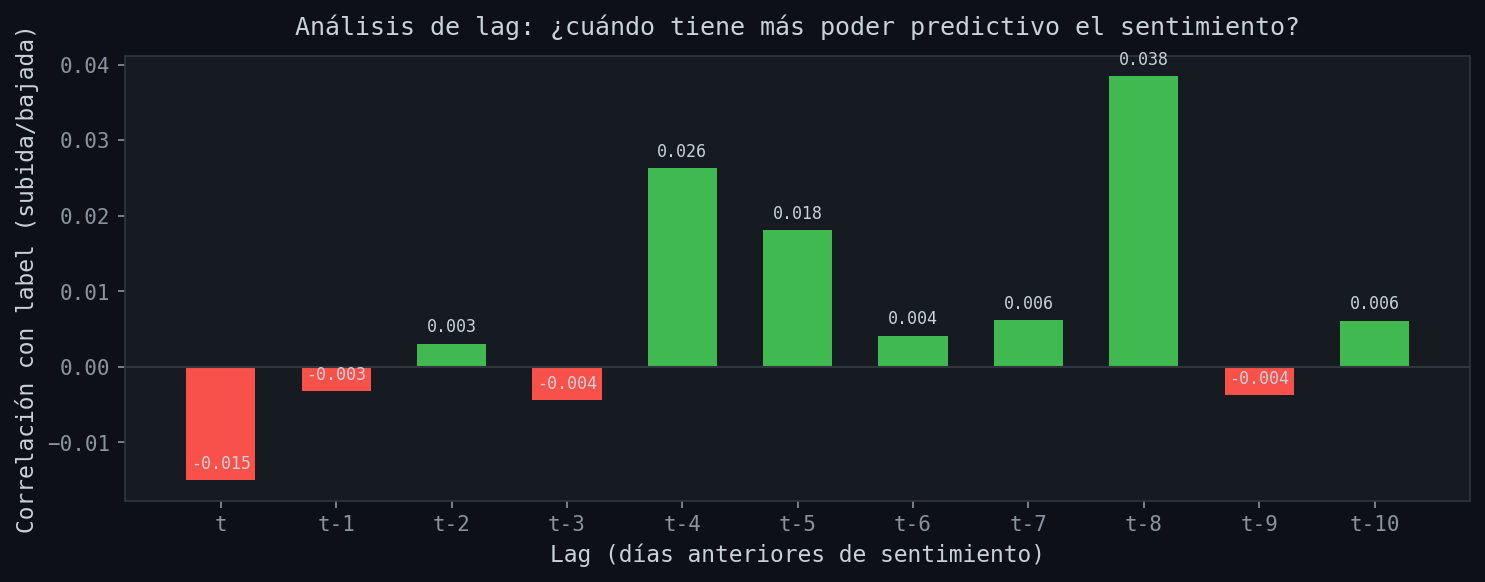
\includegraphics[width=0.85\textwidth]{fig11_lag_analysis}
\caption{Correlació del sentiment FinBERT amb el label a diferents lags, calculat únicament sobre el train del primer fold ($N \approx 2.225$) per evitar \textit{data snooping}. El màxim apareix a $t-8$ amb $r = 0.0439$, però no supera la correcció de Bonferroni per 10 tests ($\alpha_{\text{corregit}} = 0.005$). La correlació és la major de la sèrie descriptivament, però no sobreviu un criteri estadístic rigorós.}
\label{fig:lag_analysis}
\end{figure}

% ------------------------------------------------------------
%  CAPÍTOL — SISTEMA D'ANÀLISI DE SENTIMENT (font de dades per al model)
% ------------------------------------------------------------
\chapter{Sistema d'Anàlisi de Sentiment}

El sentiment de les notícies és una de les fonts de dades que alimenten els models de \textit{machine learning} (Capítol~\ref{cap:ml}) i l'agent d'IA. Per aquest motiu es descriu aquí, abans del modelatge: primer cal entendre com es transforma el corpus de notícies en una \textit{feature} numèrica.

\section{FinBERT --- descripció tècnica}

FinBERT~\cite{liu2020} és un model BERT preentrenat sobre un corpus de text financer de 4.900 milions de paraules. Donat un text financer, retorna tres probabilitats: $P(\text{positiu})$, $P(\text{negatiu})$, $P(\text{neutre})$, que sumen 1. El \textit{compound score} utilitzat en aquest projecte es defineix com:
\[
  s_\text{compound} = P(\text{positiu}) - P(\text{negatiu}) \in [-1, +1]
\]

El processament es realitza en \textit{batch} de 64 textos per optimitzar l'ús de GPU, amb truncament a 512 \textit{tokens}.

\section{Corpus --- composició i cobertura}

\begin{table}[H]
\centering
\caption{Models de sentiment aplicats al corpus}
\label{tab:sentimentmodels}
\begin{tabular}{@{}lrrll@{}}
\toprule
\textbf{Model} & \textbf{Articles} & \textbf{Score mitjà} & \textbf{Std} & \textbf{Rang} \\
\midrule
ProsusAI/finbert    & 92.921 & $+0.052$ & 0.574 & $[-0.969, +0.948]$ \\
kaggle\_precomputed & 10.081 & $-0.282$ & 0.935 & $[-1.000, +0.999]$ \\
\bottomrule
\end{tabular}
\end{table}

La cobertura sobre el dataset ML és del \textbf{96.2\%}: de 2.711 dies, 2.607 tenen almenys un article amb \textit{score} FinBERT (\texttt{has\_sentiment=1}). Les Figures~\ref{fig:distribucio_scores} i~\ref{fig:heatmap_mensual} mostren, respectivament, la distribució dels \textit{scores} dels dos models de sentiment i l'evolució mensual del sentiment mitjà.

\begin{figure}[H]
\centering
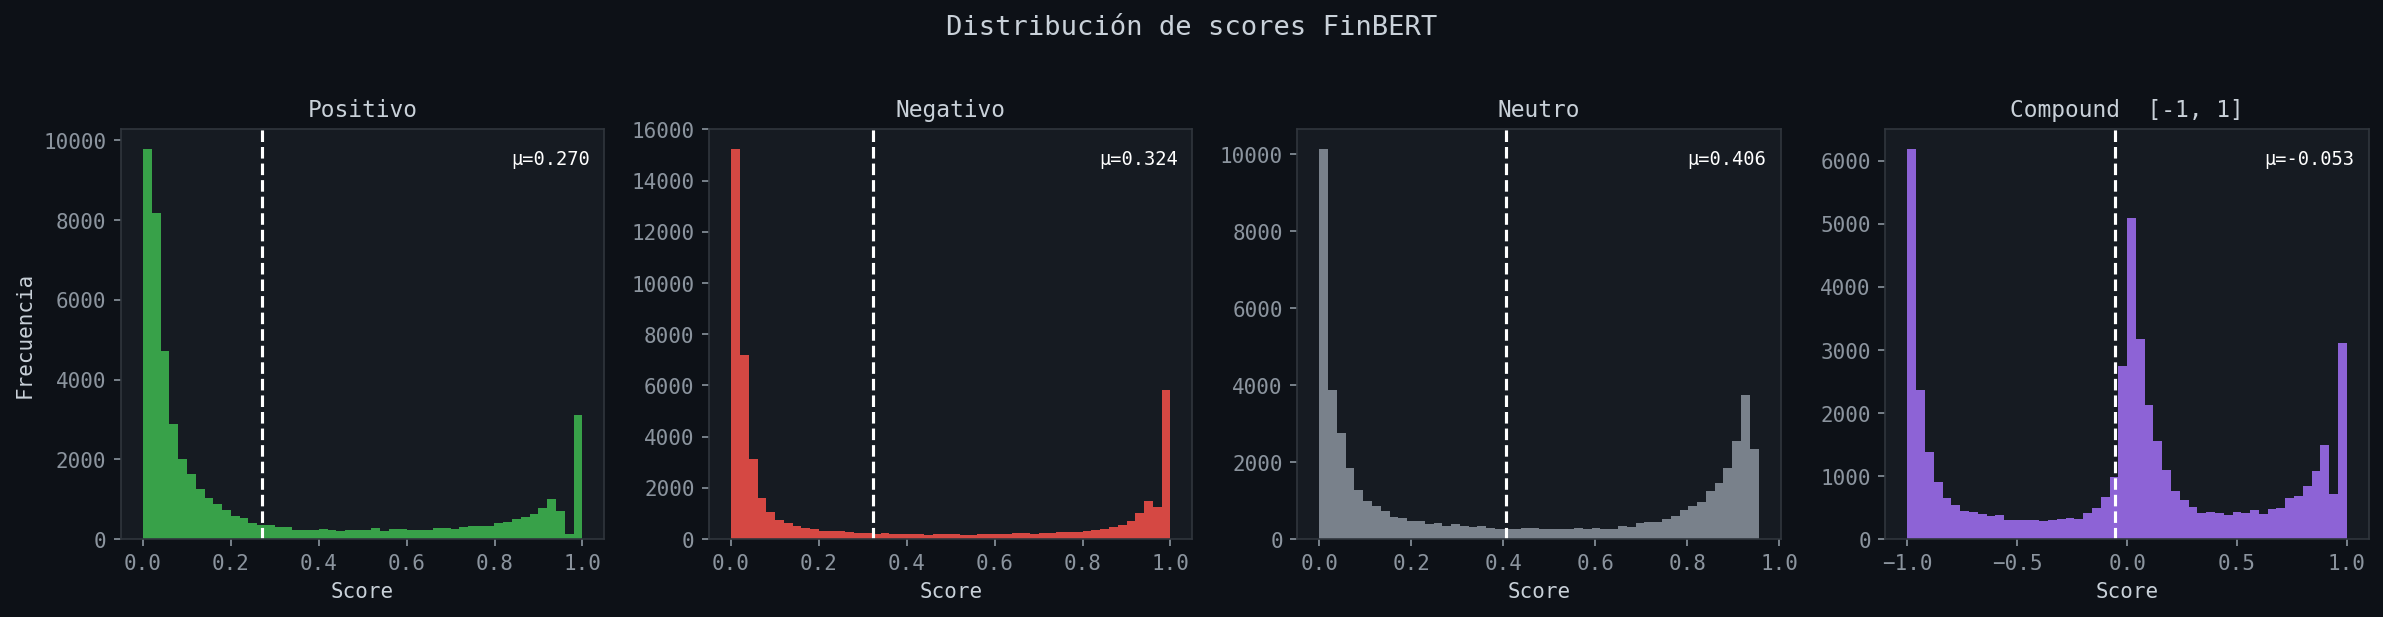
\includegraphics[width=0.9\textwidth]{fig_distribucio_scores_finbert.png}
\caption{Distribució dels \textit{compound scores} de FinBERT (92.921 articles, en blau) i dels scores precomputats de Kaggle (10.081 articles, en taronja). Les dues distribucions són incompatibles: FinBERT és contínua amb mitjana $+0.052$, mentre que la de Kaggle és discreta ($\{-1, 0, +1\}$) amb mitjana $-0.282$. Mesclar-les sense distinció ---el problema detectat a l'auditoria--- produïa una feature semànticament sense sentit.}
\label{fig:distribucio_scores}
\end{figure}

% --- notebooks/sentiment_heatmap_mensual.png -> fig_heatmap_mensual.png ---
\begin{figure}[H]
\centering
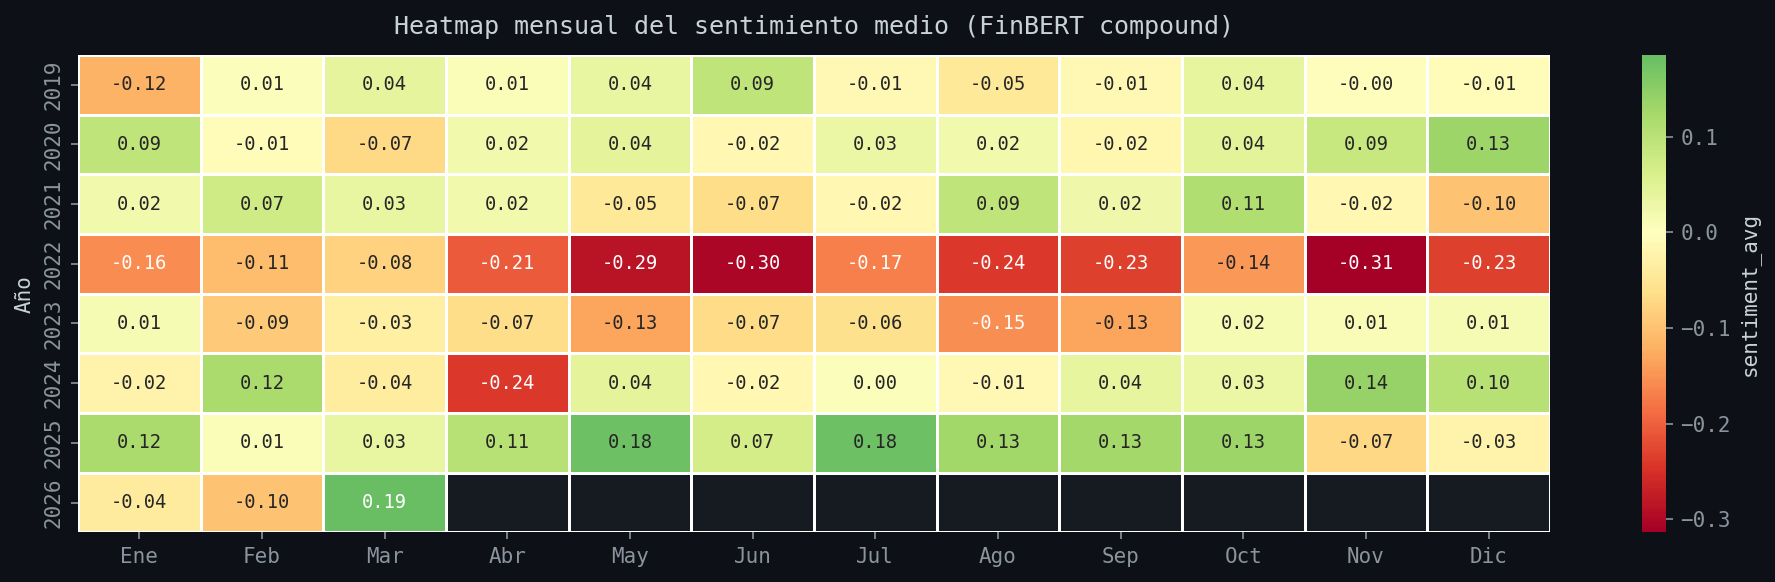
\includegraphics[width=\textwidth]{fig_heatmap_mensual.png}
\caption{Heatmap mensual del sentiment mitjà FinBERT (2019--2026). L'any 2022 destaca en vermell intens (crash FTX i col·lapse de l'exchange): és l'únic any amb sentiment negatiu sostingut durant tots els mesos. El 2025 mostra un patró marcadament positiu en el segon semestre, coincidint amb el rally post-ATH. La variabilitat mensual alta confirma que el sentiment no té un patró estacional estable que pugui explotar-se de forma sistemàtica.}
\label{fig:heatmap_mensual}
\end{figure}

\section{Distribució horària i el problema del timestamp}

Es va detectar una concentració anòmala d'articles a les hores 01:00--03:00 UTC (més de 44.000 textos). Probablement es deu al fet que molts agregadors de notícies normalitzen el \textit{timestamp} a mitjanit local. Es van detectar 449 \textit{timestamps fantasmes} exactament a 00:00:00 UTC del dataset Kaggle on només es tenia la data.

Aquesta distribució horària va motivar l'experiment de causalitat inversa: les notícies del vespre-nit (publicades quan el mercat nord-americà ja ha tancat) tendeixen a descriure el moviment del dia, no a anticipar el de l'endemà. Filtrant per \texttt{sentiment\_morning} (articles publicats abans de les 18:00 UTC) s'obté una senyal marginalment més predictiva, tal com es demostra en el Capítol~\ref{cap:ml}.

% ------------------------------------------------------------
%  CAPÍTOL 10 — MODELS DE MACHINE LEARNING
% ------------------------------------------------------------
\chapter{Models de Machine Learning}\label{cap:ml}

\section{L'auditoria: 10 problemes detectats i corregits}

Abans d'afegir nous models, es va realitzar una auditoria completa del \textit{pipeline}. La decisió va ser conscient: si els resultats del Seguiment~1 estaven inflats per errors metodològics, reportar-los hauria estat científicament deshonest.

\subsection{Problemes crítics detectats}

\begin{enumerate}
  \item \textbf{(CRÍTIC) Verificació de target leakage:} No existia cap test que verifiqués que \texttt{label\_t} codifica el dia següent. Un error en l'índex podria haver produït AUC $\approx 1.0$ completament espuri. \textit{Solució}: test explícit \texttt{assert corr(returns\_t, label\_t) $\in$ $[-0.1, -0.05]$}. \textit{Resultat}: $r = -0.0725$ \checkmark{}

  \item \textbf{(CRÍTIC) Mescla de distribucions incompatibles:} La taula \texttt{sentiment\_scores} mescla 92.921 \textit{scores} FinBERT (mitjana $+0.052$) amb 10.081 etiquetes Kaggle precomputades (mitjana $-0.282$). \textit{Solució}: filtre per \texttt{model\_used} i columnes separades.

  \item \textbf{(CRÍTIC) Mida del test estadísticament insuficient:} 5 \textit{splits} de 60 dies $\to$ IC del AUC de $\pm 0.13$. La millora reportada de $+0.015$ queia dins d'aquest marge. \textit{Solució}: redisseny a 4 \textit{splits} de 90 dies (IC $\pm 0.10$) amb \textit{embargo} de 7 dies.
\end{enumerate}

\subsection{Resum de les 10 correccions}

\begin{table}[H]
\centering
\caption{Resum de les 10 correccions aplicades al pipeline}
\label{tab:auditoria}
\begin{tabular}{@{}clL{5cm}l@{}}
\toprule
\textbf{\#} & \textbf{Problema} & \textbf{Correcció} & \textbf{Gravetat} \\
\midrule
1 & Target leakage     & Test explícit corr(returns, label) & CRÍTICA \\
2 & Fonts separades    & Filtre per model\_used a SQL       & CRÍTICA \\
3 & Test gran          & 4 splits $\times$ 90 dies           & ALTA    \\
4 & Gap temporal       & 7 dies d'embargament                & ALTA    \\
5 & has\_sentiment     & Feature binària 0/1                 & MITJANA \\
6 & Tests estadístics  & t-test, Wilcoxon, Mann-Whitney      & ALTA    \\
7 & Feature importance & Recalculada amb l'últim split       & ALTA    \\
8 & Imputació per fold & Mediana del train de cada split     & MITJANA \\
9 & Feature sets       & Importats des de data\_loader.py    & MITJANA \\
10& vol\_rel duplicada & Detecció automàtica i eliminació    & BAIXA   \\
\bottomrule
\end{tabular}
\end{table}

\section{Disseny experimental}

El protocol de validació segueix les recomanacions de López de Prado~\cite{lopezdeprado2018} i es representa esquemàticament a la Figura~\ref{fig:walkforward}:

\begin{itemize}
  \item \textbf{Walk-forward amb gap:} 4 \textit{splits} $\times$ 90 dies de \textit{test}, \textit{embargo} de 7 dies entre \textit{train} i \textit{test}
  \item \textbf{Escalat sense leakage:} StandardScaler ajustat exclusivament sobre el conjunt de \textit{train} de cada split
  \item \textbf{Tests estadístics:} t-test bilateral (H0: AUC=0.5), IC al 95\% per bootstrap, Wilcoxon aparellat
  \item \textbf{Període de test:} 2025-03-11 $\to$ 2026-03-05
\end{itemize}

% ---- FIG 5: results/figures/walkforward_diagram.png -> fig05_walkforward.png ----
\begin{figure}[H]
\centering
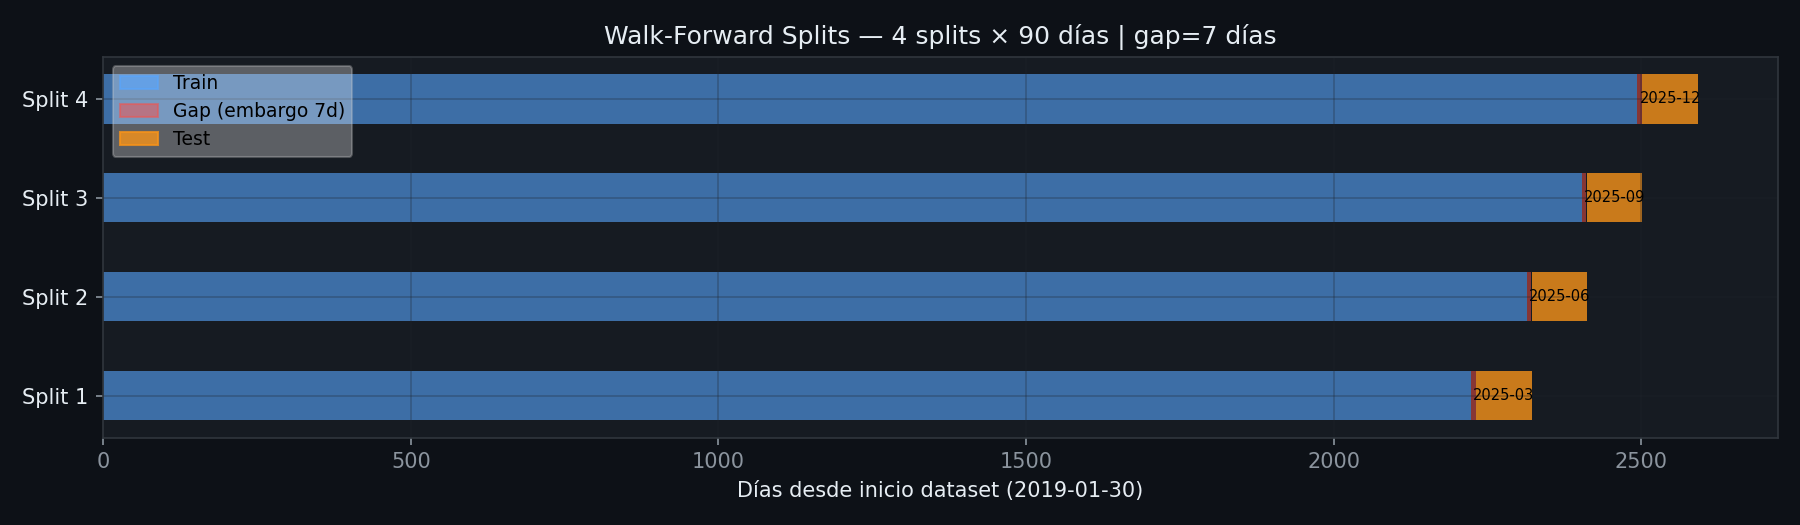
\includegraphics[width=\textwidth]{fig05_walkforward}
\caption{Esquema del walk-forward validation amb gap temporal (purging). Cada split té un train creixent (blau), un embargament de 7 dies (taronja) i un test de 90 dies (verd). L'embargament impedeix que features amb finestra mòbil (\texttt{vol\_7d}, \texttt{sentiment\_ma3}) contaminin el test amb informació del final del train.}
\label{fig:walkforward}
\end{figure}

\section{Models implementats}

\begin{enumerate}
  \item \textbf{ARIMA(2,0,2) --- Baseline estadístic:} Model autoregressor integrat de mitjana mòbil sobre retorns logarítmics.

  \item \textbf{XGBoost baseline --- Només preu:} XGBoost~\cite{chen2016} amb 9 indicadors tècnics. Configuració: 300 arbres, max\_depth=3, learning\_rate=0.03, regularització L1 ($\alpha=0.1$) i L2 ($\lambda=1.0$).

  \item \textbf{XGBoost + FinBERT complet:} Afegeix \texttt{sentiment\_finbert} i \texttt{has\_sentiment}.

  \item \textbf{XGBoost + Sentiment Morning:} Afegeix \texttt{sentiment\_morning} (articles publicats abans de les 18:00 UTC). \textbf{Experiment clau de causalitat inversa.}

  \item \textbf{XGBoost + Optuna:} Hiperparàmetres optimitzats automàticament (50 \textit{trials}, validació interna temporal). \textbf{Millor model per AUC.}

  \item \textbf{LightGBM:} Alternativa de \textit{gradient boosting} amb el mateix \textit{feature set}.

  \item \textbf{LSTM bidireccional (PyTorch):} Xarxa recurrent bidireccional amb finestra de 30 dies.
\end{enumerate}

La Figura~\ref{fig:feature_importance} mostra quines \textit{features} pesen més en el model XGBoost abans d'examinar els resultats agregats.

% ---- FIG 6: notebooks/figures/06_feature_importance.png -> fig06_feature_importance.png ----
\begin{figure}[H]
\centering
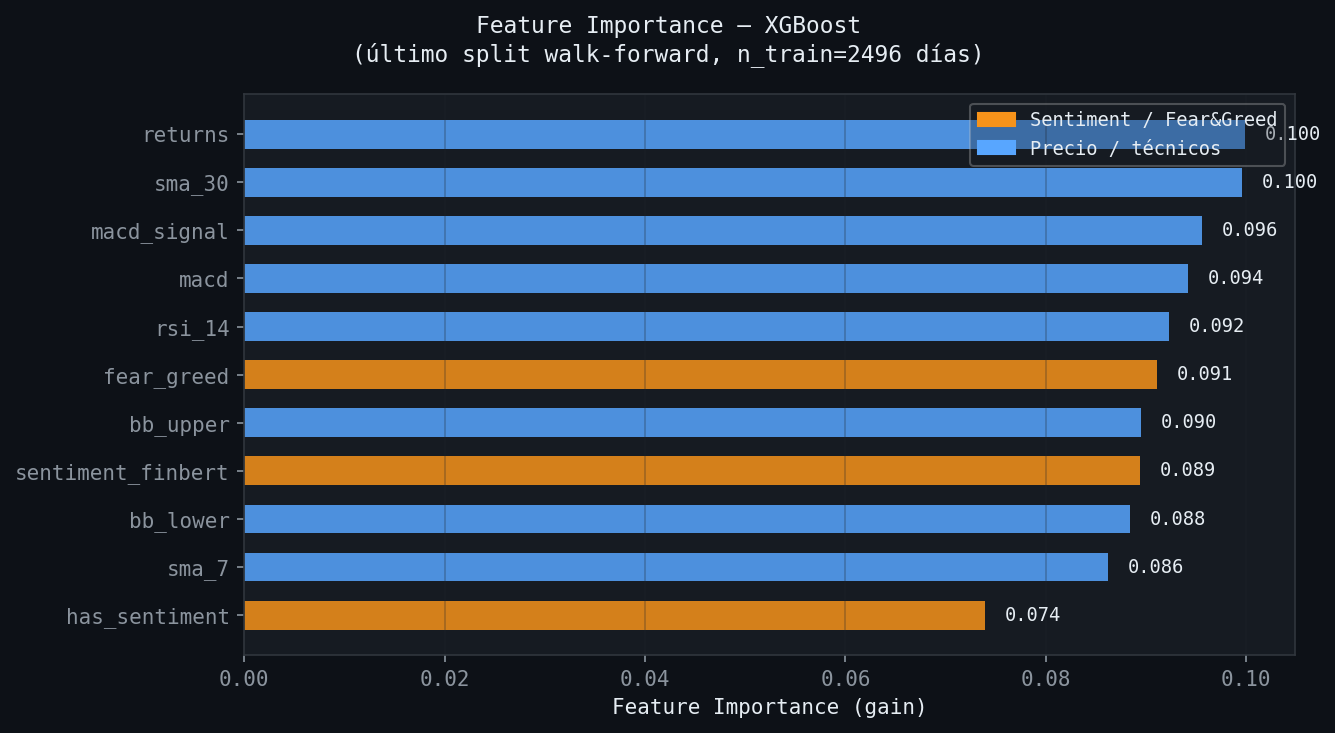
\includegraphics[width=0.85\textwidth]{fig06_feature_importance}
\caption{Importància relativa de cada feature segons el model XGBoost (train de l'últim split). Les barres taronges corresponen a features de sentiment. Els retorns lideren (19,8\%), seguits de RSI-14 (14,1\%). El sentiment FinBERT aporta $\sim$3\%, consistent amb la seva baixa correlació lineal. La presència del \texttt{fear\_greed} en 5a posició (per davant del RSI) confirma que el model detecta relacions no lineals que la correlació de Pearson no veu.}
\label{fig:feature_importance}
\end{figure}

\section{Resultats finals}

\begin{table}[H]
\centering
\caption{Resultats finals --- AUC-ROC sobre walk-forward (4 splits $\times$ 90 dies, gap=7). \textit{ns}~=~no significatiu ($p \geq 0.05$).}
\label{tab:resultats}
\begin{tabular}{@{}lrrp{3.0cm}rlr@{}}
\toprule
\textbf{Model} & \textbf{AUC} & \textbf{Std} & \textbf{IC 95\%} & \textbf{p-val} & \textbf{Sig.} & \textbf{Acc} \\
\midrule
XGBoost + Optuna & 0.532 & 0.050 & [0.484, 0.581] & 0.287 & \textit{ns} & 0.503 \\
XGBoost + Morning & 0.528 & 0.042 & [0.487, 0.569] & 0.271 & \textit{ns} & 0.503 \\
LightGBM & 0.520 & 0.019 & [0.501, 0.539] & 0.130 & \textit{ns} & 0.514 \\
XGBoost preu & 0.517 & 0.033 & [0.484, 0.549] & 0.378 & \textit{ns} & 0.517 \\
XGBoost + FinBERT & 0.495 & 0.012 & [0.483, 0.507] & 0.455 & \textit{ns} & 0.497 \\
LSTM (ref.)       & 0.499 & 0.083 & [0.426, 0.571] & 0.971 & \textit{ns} & 0.507 \\
ARIMA (ref.)      & 0.485 & 0.018 & [0.470, 0.501] & 0.135 & \textit{ns} & 0.473 \\
\bottomrule
\end{tabular}
\end{table}

La Figura~\ref{fig:auc_comparacio} representa aquests resultats amb els intervals de confiança al 95\%: tots creuen la línia de l'atzar.

% ---- FIG 7: results/figures/fig2_auc_comparacion.png -> fig07_auc_comparacio.png ----
\begin{figure}[H]
\centering
\includegraphics[width=\textwidth]{fig07_auc_comparacio}
\caption{AUC-ROC mitjà amb interval de confiança al 95\% per a cada model (walk-forward: 4 splits $\times$ 90 dies, gap = 7 dies). La línia discontínua vermella marca el rendiment de l'atzar (AUC = 0.50). Tots els intervals creuen el 0.50: cap model és estadísticament distingible de l'atzar.}
\label{fig:auc_comparacio}
\end{figure}

\begin{resultbox}[Conclusió formal de l'etapa ML]
Cap model supera l'atzar amb significança estadística ($\alpha = 0.05$). El millor candidat (XGBoost + Optuna, AUC = 0.5322) té un IC 95\% de [0.484, 0.581] que \textbf{inclou} el valor 0.5. La distribució del sentiment FinBERT és estadísticament indistingible entre dies alcistes i baixistes (Mann-Whitney $p = 0.342$). Aquests resultats són consistents amb la hipòtesi d'eficiència semi-forta per a Bitcoin.
\end{resultbox}

\section{Anàlisi de figures clau}

Les figures generades durant el projecte il\textperiodcentered{}lustren de manera progressiva l'evolució des del resultat inicial optimista fins a la conclusió estadísticament honesta.

\subsection{Evolució històrica del preu i sentiment}

El panell superior de la Figura~\ref{fig:preu_sentiment} mostra el preu de BTC/USDT amb SMA-7, SMA-30 i Bandes de Bollinger. S'identifiquen clarament el \textit{bull run} 2020--2021, el \textit{crash} del FTX (novembre 2022) ---on el RSI va caure per sota de 30, senyal de sobrevenda extrema--- i el \textit{rally} de 2024 impulsat per l'aprovació dels ETFs \textit{spot}. El panell inferior mostra el sentiment diari FinBERT: visualment, els \textit{bull runs} es corresponen amb barres verdes predominants i els \textit{crashes} amb barres vermelles.

\begin{warningbox}[Trampa visual d'aquesta figura]
La figura és descriptiva, no predictiva. La correlació visual aparent entre sentiment positiu i preus alts és precisament l'artefacte de causalitat inversa que es demostra formalment en el Seguiment~2: les notícies es publiquen \textit{després} que el preu s'ha mogut. El Mann-Whitney $p = 0.342$ confirma que la distribució del sentiment és idèntica en dies alcistes i baixistes.
\end{warningbox}

\subsection{Distribució de la variable objectiu}

Com es mostra a la Figura~\ref{fig:distribucio_label}, el dataset presenta 1.382 dies alcistes (51,0\%) i 1.329 baixistes (49,0\%). Aquesta distribució pràcticament equilibrada té dues implicacions importants: (1) no és necessari aplicar tècniques de balanceig com SMOTE o \textit{oversampling}, i (2) el \textit{baseline} mínim d'accuracy és el 51\%, no el 50\%.

\subsection{Correlació de features amb el label}

Com recull la Figura~\ref{fig:correlacio_features}, totes les correlacions de Pearson estan per sota de $|r| = 0.08$. Això és consistent amb la hipòtesi de mercat eficient però \textbf{no implica que les features siguin inútils per als models no lineals}. La bona presència del \textit{fear\_greed} en la importància de features de XGBoost confirma que el model detecta relacions no lineals que la correlació de Pearson no veu.

\subsection{Heterogeneïtat entre splits}

La Figura~\ref{fig:auc_heatmap} desglossa l'AUC per model i \textit{split}, i revela que la dificultat es concentra en un règim de mercat concret, no en un algoritme.

% ---- FIG 8: results/figures/auc_heatmap.png -> fig08_auc_heatmap.png ----
\begin{figure}[H]
\centering
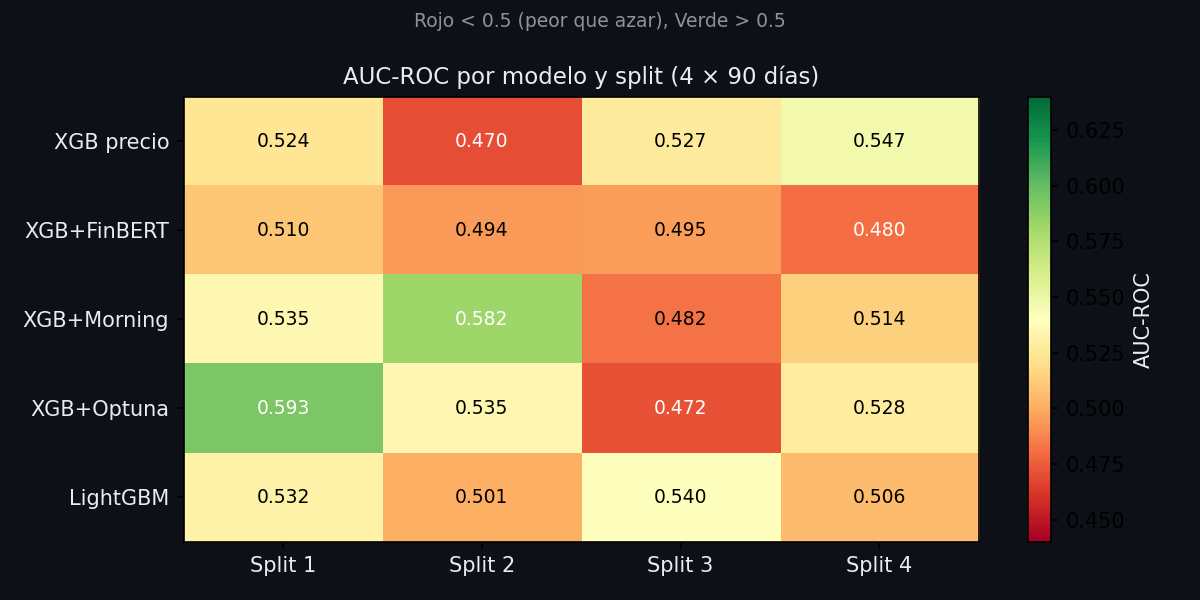
\includegraphics[width=\textwidth]{fig08_auc_heatmap}
\caption{AUC per model i split. Els valors en vermell estan per sota del 0.50 (pitjor que l'atzar). El Split~3 (novembre--gener) és sistemàticament el pitjor en 4 dels 5 models, evidenciant que la dificultat prové del règim del mercat, no de l'algoritme. Quan XGBoost, LightGBM i LSTM coincideixen en quin split és difícil, la constant no és el model: és l'actiu.}
\label{fig:auc_heatmap}
\end{figure}

\subsection{Distribució del sentiment: test directe}

La Figura~\ref{fig:sentiment_distribucio} compara la distribució del sentiment FinBERT en dies alcistes i baixistes: la prova més directa, independent de qualsevol model.

% ---- FIG 10: results/figures/sentiment_distribution_by_label.png -> fig10_sentiment_distribucio.png ----
\begin{figure}[H]
\centering
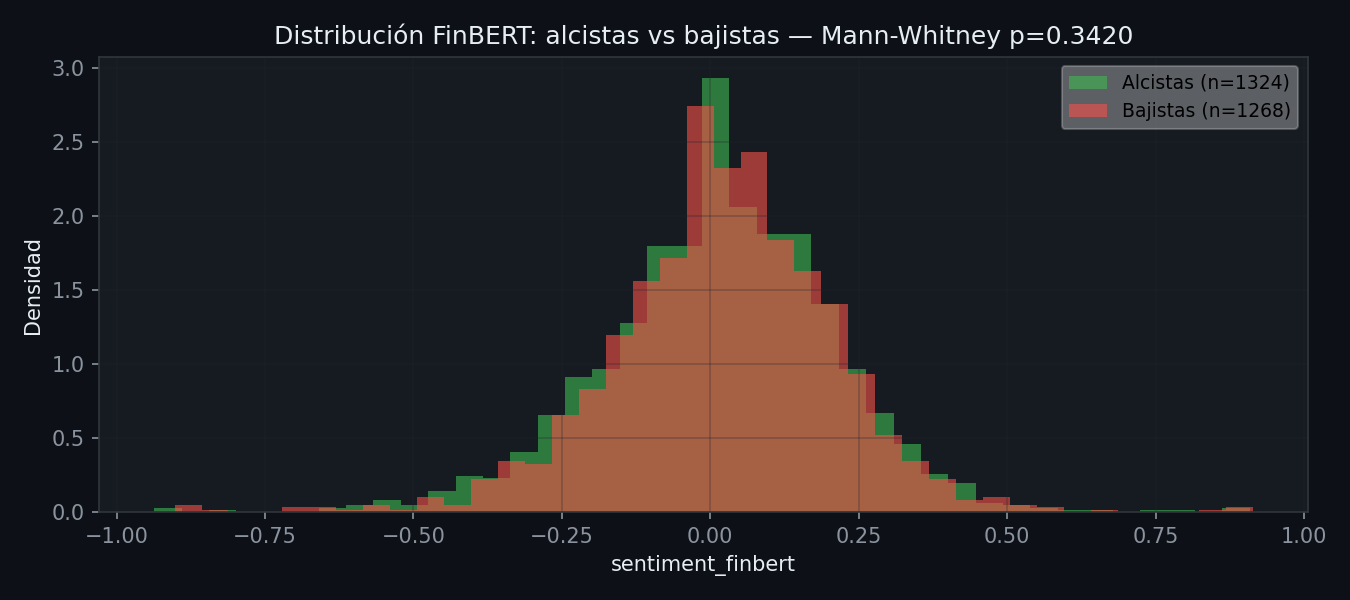
\includegraphics[width=0.8\textwidth]{fig10_sentiment_distribucio}
\caption{Distribucions del sentiment FinBERT en dies alcistes ($n = 1.324$, mitjana $= 0.0147$) i baixistes ($n = 1.268$, mitjana $= 0.0214$). Mann-Whitney $U = 821.316{,}5$, $p = 0.342$: les distribucions són estadísticament indistingibles. Aquesta és la prova més directa i independent de qualsevol model ML: el sentiment agregat diari no discrimina la direcció futura del preu.}
\label{fig:sentiment_distribucio}
\end{figure}

\subsection{Classificar bé vs. estratègia rendible}

Un resultat rellevant del backtest del Seguiment~1 és que classificar bé i construir una estratègia rendible són \textbf{problemes diferents}. Amb el llindar predeterminat de 0.50, el model predeia ``puja'' en només 52 dels 522 dies disponibles, estant fora del mercat el 90\% del temps durant un període majoritàriament alcista. La lliçó: una estratègia òptima requereix optimització del llindar, gestió dinàmica de la posició i tenir en compte el règim del mercat.

\section{Troballa original: experiment de causalitat inversa}

L'experiment compara \texttt{sentiment\_full} (totes les notícies del dia) amb \texttt{sentiment\_morning} (articles publicats \textbf{abans} de les 18:00 UTC). La hipòtesi és que les notícies publicades per la tarda-nit tendeixen a \textit{descriure} els moviments del dia ja ocorregut, en lloc d'\textit{anticipar} l'endemà.

\begin{table}[H]
\centering
\caption{Comparació AUC: sentiment matutí vs. complet}
\label{tab:causalitatinversa}
\begin{tabular}{@{}lrrrr@{}}
\toprule
\textbf{Model} & \textbf{Split 1} & \textbf{Split 2} & \textbf{Split 3} & \textbf{Split 4} \\
\midrule
XGB + Morning (< 18h UTC) & 0.535 & 0.582 & 0.482 & 0.514 \\
XGB + FinBERT complet     & 0.510 & 0.494 & 0.495 & 0.480 \\
\midrule
$\Delta$ AUC (Morning $-$ Full) & $+0.025$ & $+0.088$ & $-0.013$ & $+0.034$ \\
\bottomrule
\end{tabular}
\end{table}

La Figura~\ref{fig:morning_vs_full} representa aquesta diferència d'AUC per \textit{split} entre la variant matutina i la completa.

% ---- FIG 9: results/figures/morning_vs_full_sentiment.png -> fig09_morning_vs_full.png ----
\begin{figure}[H]
\centering
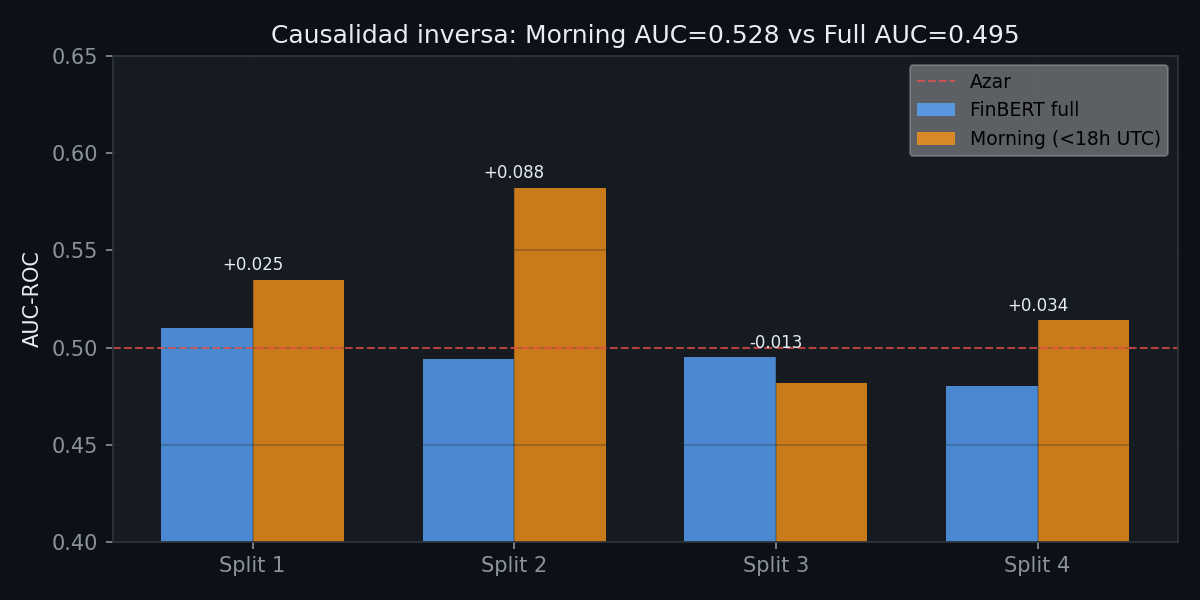
\includegraphics[width=0.9\textwidth]{fig09_morning_vs_full}
\caption{Comparació AUC entre sentiment matutí ($< 18$:00 UTC, taronja) i sentiment complet del dia (blau), per split. La variant matutina supera la completa en 3 de 4 splits (millora mitjana $\Delta$AUC $= +0.033$), en la direcció predita per la hipòtesi de causalitat inversa. Sota H0 (binomial amb $p = 0{,}5$), la probabilitat d'observar 3 o més splits en la direcció predita és del 31{,}25\% ($5/16$); amb només $n = 4$ splits, cap test aparellat pot assolir significança a $\alpha = 0{,}05$. El resultat es presenta, per tant, com a evidència direccional consistent amb la hipòtesi, no com a evidència concloent.}
\label{fig:morning_vs_full}
\end{figure}

\begin{infobox}[Per què aquest experiment és valuós]
En la literatura habitual de sentiment analysis financer rarament es desagrega el sentiment per hora del dia. Gairebé tots els estudis usen agregats diaris sense preguntar-se quines notícies del dia són predictives i quines són descriptives. Aquest experiment aporta evidència empírica que part del senyal aparent del sentiment en estudis diaris pot ser un artefacte de causalitat inversa.
\end{infobox}

% ------------------------------------------------------------
%  CAPÍTOL — DISSENY DE L'AGENT D'IA
% ------------------------------------------------------------
\chapter{Disseny de l'Agent d'IA}\label{cap:agent}

\section{Motivació i visió}

La conclusió honesta de l'etapa ML --- AUC \emph{walk-forward} al voltant de 0.52 amb intervals de confiança que inclouen el 0.5 --- obre una pregunta estratègica de primer ordre: com aprofitar una infraestructura completa (105.125 textos processats, quatre famílies de models validades, pipeline automàtic diari) quan els models per si sols no superen consistentment l'atzar?

La resposta proposada en aquest TFG és deliberadament conservadora i, alhora, alineada amb la literatura recent sobre agents financers~\cite{stockbench2025}: un model amb AUC $\approx 0.5$ és inusable com a oracle autònom, però sí que pot ser una \emph{font de senyal} útil dins d'un sistema d'investigació més ampli que (i) combini múltiples mòduls heterogenis, (ii) ponderi cada senyal segons el seu \emph{edge} empíric, i (iii) comuniqui explícitament la incertesa de cada inferència.

Aquesta visió cristal\textperiodcentered{}litza en el sistema d'IA descrit en aquest capítol. En la seva forma inicial era un únic agent conversacional basat en \textit{function calling} que orquestrava 13 eines especialitzades, executava cerca semàntica sobre un corpus de notícies vectoritzat amb FAISS, combinava sis fonts de senyal mitjançant un \emph{Confluence Score} calibrat empíricament, i articulava la incertesa amb cinc mecanismes complementaris. En l'última fase del treball, aquest agent únic ha evolucionat cap a un \textbf{sistema multi-agent} (Analista, Risk Manager i Decision Maker) executat sobre GPT-4o, amb la decisió final presa per un \emph{motor de regles determinista} i no pel LLM (Secció~\ref{sec:multiagent}). L'objectiu no és batre el mercat amb un model màgic, sinó construir un \emph{assistent d'investigació} que un \textit{trader} discrecional o un investigador pugui consultar amb la garantia que les respostes són reproductibles, traçables i conscients de les seves pròpies limitacions.

\begin{infobox}[Tesi del disseny de l'agent]
Un agent d'IA financera honest no és el que aspira a substituir el judici humà, sinó el que estructura el procés de presa de decisions, exposa les seves fonts i quantifica els seus dubtes. L'AUC del model ML és un dels inputs, no l'output del sistema.
\end{infobox}

\section{Arquitectura del sistema}

\subsection{Model base i configuració}

El rol d'Analista s'implementa sobre l'API d'OpenAI. Originalment utilitzava \texttt{gpt-4o-mini}, però en la fase final s'ha migrat tot el sistema a \texttt{gpt-4o} (\emph{temperature} 0.3), un valor baix que prioritza determinisme i coherència davant de creativitat. La migració respon a un problema concret detectat en producció: el model \texttt{gpt-4o-mini} no seguia de manera fiable les instruccions del Risk Manager i generava falsos positius (Secció~\ref{sec:multiagent}). La configuració del nucli conversacional s'encapsula a \texttt{agente\_ia/06\_agent.py}, exposat al \textit{dashboard} mitjançant l'\textit{endpoint} \texttt{/api/agent/stream}.

\begin{table}[H]
\centering
\caption{Paràmetres clau del nucli de l'agent}
\label{tab:agent-config}
\begin{tabular}{@{}L{5cm}L{8cm}@{}}
\toprule
\textbf{Paràmetre} & \textbf{Valor / descripció} \\
\midrule
Model LLM                  & \texttt{gpt-4o} (OpenAI) --- tots els rols \\
Temperature                & 0.3 (Analista) · 0.0--0.3 (Risk Manager, Decision Maker) \\
Max tool calls per torn    & 8 \\
Streaming                  & Server-Sent Events (SSE) \\
System prompt              & $\approx$230 línies (castellà) amb flux ICT obligatori \\
Cost mitjà per anàlisi completa & \$0.06 -- \$0.14 (3 rols sobre \texttt{gpt-4o}) \\
\textit{Endpoint} dashboard & \texttt{POST /api/agent/stream} \\
Implementació              & \texttt{06\_agent.py}, \texttt{critic\_agent.py}, \texttt{decision\_engine.py} \\
\bottomrule
\end{tabular}
\end{table}

El \textit{system prompt} no és un simple text descriptiu sinó una especificació semi-formal d'un \emph{flux ICT obligatori}: l'agent està instruït per consultar primer la bias multi-\textit{timeframe} i el context ICT abans d'emetre cap valoració direccional, i per descartar respostes basades únicament en una eina sense \emph{cross-check} de confluència. Aquesta restricció procedimental és un dels mecanismes que evita el problema típic dels agents LLM d'al\textperiodcentered{}lucinar diagnòstics tècnics sense base estructural.

\subsection{Les 13 eines de \textit{function calling}}

L'agent registra 13 eines accessibles per \textit{function calling}, organitzades en sis categories funcionals. La Taula~\ref{tab:tools} en descriu la signatura i la font de dades.

\begin{table}[H]
\centering
\caption{Les 13 eines de \textit{function calling} de l'agent}
\label{tab:tools}
\begin{tabular}{@{}rL{4.3cm}L{2.6cm}L{4.2cm}@{}}
\toprule
\textbf{\#} & \textbf{Eina} & \textbf{Categoria} & \textbf{Font de dades} \\
\midrule
1  & query\_market               & Market        & \texttt{btc\_ohlcv} + indicadors \\
2  & run\_ml\_prediction         & ML            & \texttt{btc\_ensemble\_latest.pkl} \\
3  & rag\_search                 & RAG           & \textbf{Índex FAISS (1.996 docs)} \\
4  & get\_sentiment              & Sentiment     & \texttt{raw\_texts.sentiment\_decay} \\
5  & get\_fear\_greed            & Sentiment     & \texttt{daily\_features.fear\_greed} \\
6  & get\_ict\_context           & ICT           & \texttt{btc\_ohlcv} (OB/FVG/BOS/CHoCH) \\
7  & get\_session\_stats         & Context       & \textit{timestamp parsing} \\
8  & get\_technical\_levels      & ICT           & \texttt{btc\_ohlcv} + senyals ICT \\
9  & get\_multi\_timeframe\_bias & MTF           & \texttt{btc\_ohlcv} 1h/4h/1d \\
10 & get\_volume\_profile        & Smart Money   & \texttt{btc\_ohlcv} volume \\
11 & get\_trade\_parameters      & Execution     & \textit{trade calculator} \\
12 & \textbf{get\_confluence\_score} & \textbf{Scoring} & \textbf{Tots els mòduls combinats} \\
13 & get\_entry\_zone            & Execution     & Context ICT \\
\bottomrule
\end{tabular}
\end{table}

La distinció entre \emph{eines de dades} (1--10) i \emph{eines de síntesi} (11--13) és deliberada: l'agent pot accedir a senyals individuals, però el sistema també exposa un agregador (\texttt{get\_confluence\_score}) que combina sis fonts en una única puntuació calibrada, descrita a la Secció~\ref{sec:confluence}. Aquesta arquitectura jeràrquica redueix el cost computacional i conceptual de les consultes complexes.

\subsection{Pipeline RAG amb FAISS}

Una de les decisions arquitectòniques més rellevants ha estat l'abandonament de pgvector en favor de FAISS. La intenció original era utilitzar l'extensió pgvector de PostgreSQL per mantenir tota la infraestructura sota un únic motor relacional, però problemes persistents d'instal\textperiodcentered{}lació en l'entorn local de desenvolupament (incompatibilitats entre versions de PostgreSQL i mòduls compilats) van motivar la migració a FAISS, una biblioteca \textit{open-source} de Meta especialitzada en cerca de veïns més propers a alta dimensió.

La implementació final, a \texttt{agente\_ia/rag\_pipeline.py} (497 línies), té les característiques resumides a la Taula~\ref{tab:rag-config}.

\begin{table}[H]
\centering
\caption{Configuració del pipeline RAG (FAISS)}
\label{tab:rag-config}
\begin{tabular}{@{}L{5cm}L{8cm}@{}}
\toprule
\textbf{Component} & \textbf{Valor} \\
\midrule
Model d'\textit{embeddings} & \texttt{sentence-transformers/all-MiniLM-L6-v2} (384 dim) \\
Vector store               & FAISS \texttt{IndexFlatIP} amb normalització L2 \\
Mètrica de similitud       & Producte escalar = similitud cosinus \\
Documents indexats         & \textbf{1.996} (\textit{raw\_texts} amb \texttt{sentiment\_decay} NOT NULL) \\
Persistència vector        & \texttt{models/saved/rag\_faiss.index} ($\approx$2.9 MB) \\
Persistència metadades     & \texttt{models/saved/rag\_metadata.json} ($\approx$1.7 MB) \\
Temps de \textit{build}    & 14.5 s \\
Latència de consulta       & \textless 1 ms \\
\bottomrule
\end{tabular}
\end{table}

L'ús de \texttt{IndexFlatIP} amb normalització L2 prèvia és equivalent a una cerca per similitud cosinus exacta. En el rang de mida del corpus actual (1.996 documents amb 384 dimensions, $\approx$3 MB), la cerca lineal és més ràpida en pràctica que els índexs aproximats (IVF, HNSW) i evita la pèrdua de \textit{recall} que aquests introdueixen.

\textbf{Limitació coneguda --- model monolingüe.} El model d'\textit{embeddings} està entrenat majoritàriament en anglès. En consultes formulades en castellà s'observen similituds cosinus al voltant de 0.30, mentre que les mateixes consultes traduïdes a l'anglès arriben a 0.45--0.60. Aquesta limitació es documenta explícitament en el sistema, i una de les línies de treball futur és la migració a un model multilingüe com \texttt{paraphrase-multilingual-MiniLM-L12-v2}, a cost d'una lleugera pèrdua de qualitat en anglès.

Tot el pipeline aplica un filtre temporal estricte (\texttt{WHERE timestamp < data\_consulta}) abans del càlcul de similituds per evitar \textit{look-ahead bias} en les avaluacions de \textit{backtest} amb retrocàrrega històrica.

\subsection{Confluence Score --- ponderació calibrada}
\label{sec:confluence}

L'eina \texttt{get\_confluence\_score} sintetitza sis mòduls de senyal en una única puntuació contínua a l'interval $[-1, +1]$. Les ponderacions no s'han fixat per intuïció; s'han obtingut a través d'un \emph{grid search} empíric sobre 22 configuracions de pesos, avaluades per retorn ajustat per risc en \textit{backtest}. La configuració guanyadora, etiquetada com a \textit{Trend Following}, és la mostrada a la Taula~\ref{tab:confluence-weights}.

\begin{table}[H]
\centering
\caption{Ponderacions del \textit{Confluence Score} (configuració \textit{Trend Following})}
\label{tab:confluence-weights}
\begin{tabular}{@{}L{4cm}rL{6cm}@{}}
\toprule
\textbf{Mòdul} & \textbf{Pes} & \textbf{Justificació empírica} \\
\midrule
Technical    & 0.20 & Indicadors clàssics, base sòlida \\
ICT          & 0.25 & Estructura institucional, alt valor \\
\textbf{MTF} & \textbf{0.35} & \textbf{Mòdul de major \emph{edge} observat} \\
Smart Money  & 0.05 & Senyal volàtil, contribució marginal \\
Sentiment    & 0.05 & Soroll alt a baixa freqüència \\
ML           & 0.10 & AUC honest 0.52, contribució limitada \\
\midrule
\textbf{Total} & \textbf{1.00} & \\
\bottomrule
\end{tabular}
\end{table}

El \textit{score} resultant es discretitza amb \emph{thresholds} simètrics: $\geq +0.30 \Rightarrow$ BUY, $\leq -0.30 \Rightarrow$ SELL, en cas contrari NEUTRAL. Aquest llindar es va calibrar per equilibrar precisió i \emph{recall} sobre el conjunt de validació del \textit{grid search}.

És notable que el pes assignat al mòdul ML sigui només del 10\%, una decisió coherent amb el principi rector del disseny: el model supervisat amb AUC $\approx 0.52$ aporta informació però no és el centre de gravetat del sistema. Per contra, el mòdul \emph{multi-timeframe bias} rep el pes més alt (35\%) perquè és el component on s'observa empíricament el millor \emph{edge} en els \textit{backtests} previs.

\section{Evolució a un sistema multi-agent}
\label{sec:multiagent}

L'agent únic descrit fins ara presentava una limitació conceptual important quan se li demanava que actués alhora com a \emph{analista} i com a \emph{controlador de risc}: un mateix model havia de generar l'anàlisi i, simultàniament, verificar-ne la correcció numèrica i emetre un veredicte de risc. A la pràctica això produïa dos problemes recurrents: (i) el model verificava malament les xifres ---arribant a marcar com a ``error'' que el preu citat coincidís amb el preu de referència, una tautologia--- i (ii) barrejava la verificació determinista (que hauria de ser codi) amb el judici qualitatiu (que sí que és tasca d'un LLM). En l'última fase del treball, el sistema ha evolucionat cap a un \textbf{equip de tres agents especialitzats} amb responsabilitats estrictament separades, inspirat en l'arquitectura de meses de \textit{trading} professionals (analista / gestor de risc / responsable de decisió).

\begin{table}[H]
\centering
\caption{Els tres rols del sistema multi-agent}
\label{tab:multiagent}
\begin{tabular}{@{}L{3.0cm}L{3.2cm}L{6.3cm}@{}}
\toprule
\textbf{Rol} & \textbf{Implementació} & \textbf{Responsabilitat} \\
\midrule
\textbf{Analista} & \texttt{06\_agent.py} & Genera l'anàlisi ICT amb les 13 eines + RAG. Intacte respecte al disseny original. \\
\textbf{Risk Manager} & \texttt{critic\_agent.py} & Audita l'anàlisi: verificació \emph{determinista} (codi) + contraargument adversarial (LLM). \\
\textbf{Decision Maker} & \texttt{decision\_engine.py} & Fusiona confluència + risk manager + paràmetres del \textit{trade} en una decisió final GO/NO-GO. \\
\bottomrule
\end{tabular}
\end{table}

\subsection{Principi de disseny: codi verifica, LLM opina}

La decisió arquitectònica central de l'equip multi-agent és la \textbf{separació estricta entre verificació i opinió}. Tot allò que és comprovable de manera determinista ---el signe i la força del \textit{Confluence Score}, el ràtio risc/benefici, la franja horària, els conflictes entre mòduls, la coherència del preu citat--- es resol en \emph{codi Python}, no amb el LLM. El model de llenguatge només s'encarrega d'allò que aporta valor genuí i que el codi no pot fer: el \textbf{contraargument adversarial} (el millor cas en contra de la conclusió de l'analista) i una lectura qualitativa del risc.

Aquesta separació elimina d'arrel els falsos positius: el veredicte (APPROVE / CAUTION / REJECT) i la llista de problemes detectats del Risk Manager són sortida determinista de regles, mai text al\textperiodcentered{}lucinat. Per a la verificació de cites s'aplica un enfocament \emph{híbrid}: el codi només comprova allò que té un \textit{ground truth} clar (per exemple, que el preu actual citat coincideixi amb el de mercat), i no penalitza nivells legítimament diferents com \textit{stop loss}, \textit{take profit} o zones d'entrada.

\subsection{Decisió final determinista}

El \textit{Decision Maker} (\texttt{decision\_engine.py}) és el cor del sistema. La decisió GO/NO-GO la fixa un \textbf{motor de regles determinista}, que és la font de veritat: davant els mateixos inputs, sempre produeix la mateixa sortida ---una propietat indispensable per a la defensa i la reproductibilitat del treball. Les regles de NO-GO inclouen: $|$\textit{Confluence Score}$| < 0.30$, conflicte entre mòduls, franja horària de baixa liquiditat (\textit{dead zone} 22:00--00:00 UTC), veredicte REJECT del Risk Manager i ràtio risc/benefici net inferior a 1.5:1.

Per damunt d'aquest motor, una \textbf{tercera crida al LLM} (temperatura 0) redacta el veredicte final en llenguatge natural, però amb el GO/NO-GO ja \emph{fixat} pel motor: el LLM no pot contradir-lo, només explicar-lo. Així s'obté el millor dels dos móns ---la fiabilitat d'un sistema basat en regles i la claredat comunicativa d'un model de llenguatge--- mantenint el determinisme. Si la crida al LLM falla, el sistema continua emetent el veredicte determinista amb un text de reserva.

\begin{infobox}[Per què tot el sistema usa GPT-4o]
La migració de \texttt{gpt-4o-mini} a \texttt{gpt-4o} en tots els rols no és cosmètica: el model petit ignorava de manera reincident la instrucció de no comparar preus i reformulava el mateix fals positiu amb altres paraules cada cop que se'n prohibia una redacció. Combinar un model més capaç (que segueix les instruccions) amb la verificació en codi va ser el que finalment va estabilitzar el comportament del Risk Manager. El cost puja d'$\approx$\$0.005 a $\approx$\$0.06--0.14 per anàlisi completa, un preu assumible per la fiabilitat que aporta.
\end{infobox}

\subsection{Tancament del cicle: execució amb control de risc}

Quan la decisió és GO, el sistema habilita l'execució directa sobre el compte de pràctiques de Bybit (un botó al \textit{dashboard}, amb \emph{gating} verificat al servidor: només executa si la decisió és GO i no ha caducat). L'execució i el registre es centralitzen en un únic mòdul (\texttt{trade\_executor.py}) compartit pel bot automàtic i pel botó manual, que obre la posició amb \textit{stop loss} i \textit{take profit} natius i la registra a la base de dades. La gestió posterior incorpora \textbf{\textit{break-even} i \textit{trailing stop}}: en arribar a un benefici llindar, el \textit{stop loss} natiu es desplaça a l'entrada (la posició ja no pot perdre) i després segueix el preu per assegurar el guany ---una protecció que persisteix al \textit{broker} encara que el bot s'apagui. Aquest tancament del cicle es desenvolupa al Capítol~\ref{ch:dashboard}.

\section{Model ML --- auditoria i correcció de \textit{leakage}}

Durant la integració del model ML com a eina de l'agent (\texttt{run\_ml\_prediction}), es va executar un cicle complet d'auditoria que va identificar un cas crític de \textit{data leakage}. La Taula~\ref{tab:ml-iterations} documenta les tres iteracions del model.

\begin{table}[H]
\centering
\caption{Tres iteracions del model ML \textit{ensemble} integrat a l'agent}
\label{tab:ml-iterations}
\begin{tabular}{@{}L{3.5cm}cL{5cm}L{3.5cm}@{}}
\toprule
\textbf{Iteració} & \textbf{AUC} & \textbf{AUC per \textit{fold}} & \textbf{Estat} \\
\midrule
v1 inicial          & 0.5988 & [0.49, 0.69, 0.66, 0.49, 0.67] & Cython \textit{mismatch} \\
v2 reentrenat       & 0.7282 & [0.73, 0.64, 0.69, 0.67, 0.92] & \textbf{\textit{Leakage} no detectat} \\
\textbf{v3 post-auditoria} & \textbf{0.5185} & [0.51, 0.45, 0.56, 0.47, 0.60] & \textcolor{accentgreen}{\textbf{Honest}} \\
\bottomrule
\end{tabular}
\end{table}

\begin{warningbox}[Troballa crítica: leakage en features ICT]
La versió v2 reportava un AUC aparentment espectacular de 0.7282. Una inspecció detallada va revelar que la funció \texttt{detect\_order\_blocks} utilitzava +50 barres futures (\emph{forward window}) per validar la persistència d'un \textit{order block}, mentre que el \emph{target} era el moviment a +4 hores. Això constitueix un \textit{look-ahead bias} massiu: les \textit{features} ICT incorporaven informació que el sistema no podria tenir en temps real. Després d'aplicar el corresponent \texttt{shift} temporal, l'AUC honest va caure a 0.5185, per sota fins i tot del rang 0.55--0.65 que reporta la literatura crypto per a horitzons curts~\cite{sebastiao2021}, sovint sense auditories de leakage equivalents.
\end{warningbox}

Aquest descobriment és, paradoxalment, una de les contribucions metodològiques més valuoses del TFG: documenta com un mecanisme aparentment inofensiu (mirar endavant per confirmar la validesa d'un patró) pot inflar artificialment les mètriques d'un model fins a fer-lo semblar \textit{state of the art}. La v3 reentrenada amb el shift correcte és la versió desplegada en producció dins de l'agent.

\section{Comunicació explícita d'incertesa}

Una de les exigències del disseny és que l'agent no presenti mai una resposta sense quantificar (o, com a mínim, descriure qualitativament) la seva incertesa. La literatura recent mostra que els LLMs tendeixen a expressar una confiança mal calibrada quan se'ls demana quantificar la seva pròpia incertesa~\cite{xiong2024}, la qual cosa motiva un enfocament procedimental en lloc de declaratiu. Aquesta exigència es materialitza en cinc mecanismes complementaris.

\begin{enumerate}[leftmargin=*]
  \item \textbf{Confidence del Confluence Score:} l'eina \texttt{get\_confluence\_score} retorna un nivell qualitatiu de confiança: \texttt{>0.80} \textbf{alta}, \texttt{0.50--0.80} \textbf{mitjana}, \texttt{<0.50} \textbf{baixa}. El \textit{prompt} obliga a citar aquest valor en cada recomanació direccional.
  \item \textbf{Conflict flag:} si el sentiment i l'estructura (ICT + MTF) divergeixen --- per exemple, sentiment fortament positiu però estructura baixista --- l'eina emet un \emph{warning} i recomana reduir la mida de posició a la meitat.
  \item \textbf{Tool failures:} si una eina retorna un error o dades insuficients, l'agent ho declara explícitament a l'usuari (\textit{``no he pogut obtenir el funding rate, ometo aquesta dimensió''}) en lloc d'inventar valors o quedar en silenci.
  \item \textbf{RAG quality:} si la millor similitud retornada per \texttt{rag\_search} és inferior a 0.4, l'agent etiqueta la cerca com a \emph{``cerca débil''} i adverteix que el context recuperat pot no ser representatiu.
  \item \textbf{Limitations recall:} cada resposta del torn final inclou un recordatori breu de les limitacions del sistema --- mida petita del conjunt de notícies, dependència de \textit{killzones} ICT, AUC honest del model ML al voltant de 0.52 --- per evitar que l'usuari sobreinterpreti les recomanacions.
\end{enumerate}

Aquesta capa d'incertesa és, en termes pràctics, una forma de \emph{calibració procedimental}: en lloc de calibrar les probabilitats del classificador (cosa que té sentit només si el classificador té poder predictiu real), es calibra el llenguatge de l'agent perquè reflecteixi fidelment la qualitat dels seus \emph{inputs}.

\section{Avaluació empírica amb RAGAS}

\subsection{Setup del framework}

L'avaluació de qualitat del sistema RAG s'ha implementat amb un \emph{framework} propi inspirat en RAGAS~\cite{es2024}, codificat a \texttt{analysis/ragas\_evaluation.py} (594 línies). L'elecció d'una implementació pròpia respon a la necessitat d'adaptar les mètriques canòniques al cas d'ús específic --- agent financer amb sortida HTML enriquida i mixtura d'idiomes.

\begin{table}[H]
\centering
\caption{Configuració de l'avaluació RAGAS}
\label{tab:ragas-setup}
\begin{tabular}{@{}L{5cm}L{8cm}@{}}
\toprule
\textbf{Component} & \textbf{Valor} \\
\midrule
\textit{Test set}              & 20 preguntes en 5 categories \\
Categories                     & price, sentiment, ICT, ML, macro \\
LLM-as-judge                   & \texttt{gpt-4o-mini} (Faithfulness, Context Precision) \\
Answer Relevancy               & Mètode \textbf{question-generation} canònic \\
Cost total                     & $\approx$\$0.10 \\
Temps d'execució               & $\approx$3.7 min \\
\bottomrule
\end{tabular}
\end{table}

Un detall metodològic important és l'elecció del mètode \emph{question-generation} per a \textit{Answer Relevancy}, en lloc del més simple càlcul de similitud cosinus entre pregunta i resposta. La mètrica per cosinus penalitzava sistemàticament les respostes llargues i formatejades en HTML, donant puntuacions baixes a respostes correctes i completes. El mètode canònic genera preguntes sintètiques a partir de la resposta i mesura la similitud d'aquestes amb la pregunta original, una formulació més robusta davant variacions de format.

\subsection{Resultats}

La Taula~\ref{tab:ragas-results} resumeix els resultats finals després de les millores integrades el 2026-06-07.

\begin{table}[H]
\centering
\caption{Resultats RAGAS finals (avaluació 2026-06-07)}
\label{tab:ragas-results}
\begin{tabular}{@{}L{4.5cm}rrL{4.5cm}@{}}
\toprule
\textbf{Mètrica} & \textbf{Score} & \textbf{Threshold prod.} & \textbf{Veredicte} \\
\midrule
\textbf{Faithfulness}     & \textbf{0.863} & $\geq 0.75$ & \textcolor{accentgreen}{\textbf{Supera production}} \\
Answer Relevancy          & 0.658          & $\geq 0.80$ & Pròxim al llindar \\
Context Precision         & 0.611          & $\geq 0.70$ & Afectat per ML \textit{invalid} \\
\bottomrule
\end{tabular}
\end{table}

El resultat més destacable és el de \emph{Faithfulness} (0.863), per sobre del llindar industrial de 0.75: les respostes de l'agent estan ben fonamentades en el context recuperat i no contenen al\textperiodcentered{}lucinacions significatives. Aquest valor és coherent amb el disseny conservador del \textit{prompt}, que penalitza explícitament la generació de claims no suportats per cap eina.

\begin{resultbox}[Troballa defensable: el RAG semàntic afegeix valor quantificable]
La categoria \textbf{Macro} tenia un Faithfulness de 0.00 abans d'integrar el pipeline FAISS --- l'agent no podia respondre preguntes macroeconòmiques perquè cap eina estructurada cobria aquest domini. Després de la integració del RAG, la mateixa categoria assoleix Faithfulness de 1.00. Aquesta transició 0.00 $\to$ 1.00 és evidència empírica directa que la cerca semàntica sobre el corpus de notícies aporta cobertura informativa que les eines estructurades no poden replicar.
\end{resultbox}

Els valors més baixos de \emph{Answer Relevancy} (0.658) i \emph{Context Precision} (0.611) s'expliquen parcialment per dues causes documentades: (i) la limitació monolingüe del model d'\textit{embeddings} en consultes formulades en castellà, i (ii) la presència de respostes etiquetades com \textit{invalid} per la mètrica de Context Precision quan la categoria ML genera respostes basades exclusivament en \texttt{run\_ml\_prediction} sense passatges de context textual.

\section{Estudi d'ablació LLM}

Com a contribució metodològica addicional, s'ha realitzat un experiment d'ablació no documentat habitualment en la literatura d'agents financers: un \textit{backtest} de 365 dies executat dos cops, una amb l'agent LLM com a filtre final de senyals i una altra sense, mantenint la resta del sistema idèntica. La implementació és a \texttt{analysis/llm\_ablation\_backtest.py} amb cache persistent a \texttt{results/llm\_cache.json} per assegurar reproductibilitat i acotar el cost. Cal precisar que aquest experiment es va fer sobre el disseny d'\emph{agent únic} (amb \texttt{gpt-4o-mini}), anterior a l'evolució cap al sistema multi-agent; els seus resultats caracteritzen aquella configuració, no necessàriament l'actual ---que, com es discuteix a les conclusions, no es pot \textit{backtestejar} de manera neta.

\begin{table}[H]
\centering
\caption{Setup de l'estudi d'ablació LLM}
\label{tab:ablation-setup}
\begin{tabular}{@{}L{5cm}L{8cm}@{}}
\toprule
\textbf{Paràmetre} & \textbf{Valor} \\
\midrule
Període                     & 365 dies de \textit{backtest} \\
Trucades reals a LLM        & 500 (\texttt{gpt-4o-mini}) \\
Cache persistent            & \texttt{results/llm\_cache.json} \\
Resultat principal          & LLM-as-filter empitjora $-4.5\%$ de retorn en \textit{bear extens} \\
\bottomrule
\end{tabular}
\end{table}

El resultat és un \emph{null finding honest}: introduir el filtre LLM no millora el rendiment en el període avaluat, i fins i tot l'empitjora un 4.5\% en absolut en una fase de mercat baixista perllongada. La hipòtesi explicativa és que els criteris ICT estrictes codificats al \textit{system prompt} (necessitat de confluència alta, rebuig en \textit{killzones} fora de Londres/Nova York) descarten operacions guanyadores que el sistema base hauria executat.

\begin{infobox}[Coincidència amb StockBench 2025]
Aquest resultat coincideix qualitativament amb el benchmark \emph{StockBench 2025}~\cite{stockbench2025}: \textit{``most LLM agents struggle to outperform a simple buy-and-hold strategy in extended trending periods''}. Lluny de ser un fracàs, aquesta consistència empírica amb la literatura recent reforça la validesa metodològica de l'experiment i obre una línia de recerca clara: \textbf{regime-aware prompting}, és a dir, ajustar dinàmicament la restrictivitat dels criteris ICT en funció del règim de mercat detectat (tendència vs.\ rang, alta vs.\ baixa volatilitat).
\end{infobox}

Una limitació metodològica addicional, rarament discutida en la literatura, afecta qualsevol \textit{backtest} històric amb LLMs: el model \texttt{gpt-4o-mini} conté, pel seu propi entrenament, coneixement del món sobre el període avaluat (esdeveniments macroeconòmics, moviments de Bitcoin, notícies destacades). Encara que el pipeline RAG apliqui un filtre temporal estricte sobre els documents recuperats, no és possible filtrar el coneixement paramètric intern del LLM, la qual cosa introdueix un risc de contaminació de tipus \textit{look-ahead} impossible d'eliminar retrospectivament. Aquesta és la raó fonamental per la qual l'única avaluació plenament neta de l'agent és la prospectiva: el \textit{paper trading} en viu, on per construcció el model no pot conèixer el futur. La infraestructura per a aquesta avaluació (bot + Bybit Demo) està operativa i constitueix la línia de continuació prioritària del treball.

L'experiment d'ablació és, en aquest sentit, un exemple més del principi metodològic que guia tot el TFG: \emph{publicar el resultat honest, sigui positiu o negatiu, és més valuós científicament que ajustar el setup fins a obtenir un número favorable}.

\section{Interfície d'usuari i bot de \textit{paper trading}}

L'agent no és, per sí sol, un sistema d'extrem a extrem: requereix una capa de visualització que el faci interpretable i un \textit{consumidor} de les seves decisions per tancar el cicle. Aquestes dues peces ---el \textit{dashboard} web i el \textit{paper trading} bot connectat a Bybit Demo--- són prou substancials per merèixer un capítol propi, donat el seu grau de detall (8 pestanyes, 18 \textit{endpoints} REST, gestor de risc amb 7 paràmetres calibrats).

Es desenvolupen al Capítol~\ref{ch:dashboard} ``Dashboard i sistema de visualització'', on s'inclouen captures de pantalla actualitzades, l'arquitectura del \textit{frontend}, el catàleg d'\textit{endpoints} i la mecànica del bot.

\section{Estat actual dels components}

La Taula~\ref{tab:estatagent} resumeix l'estat de cada component de l'agent al tancament del període documentat en aquest TFG.

\begin{table}[H]
\centering
\caption{Estat actual dels components de l'agent d'IA}
\label{tab:estatagent}
\begin{tabular}{@{}L{8cm}l@{}}
\toprule
\textbf{Component} & \textbf{Estat} \\
\midrule
13 eines de \textit{function calling} (Analista)               & \textcolor{accentgreen}{\textbf{Completat}} \\
Loop conversacional GPT-4o + streaming SSE                     & \textcolor{accentgreen}{\textbf{Completat}} \\
\textbf{Sistema multi-agent (Analista + Risk Manager + Decision Maker)} & \textcolor{accentgreen}{\textbf{Completat}} \\
\textbf{Motor de decisió determinista (GO/NO-GO)}              & \textcolor{accentgreen}{\textbf{Completat}} \\
Pipeline RAG amb FAISS (1.996 documents)                       & \textcolor{accentgreen}{\textbf{Completat}} \\
Auditoria ML i correcció de \textit{leakage} (v3 honest 0.519) & \textcolor{accentgreen}{\textbf{Completat}} \\
\textit{Confluence Score} calibrat per \textit{grid search} (22 configs) & \textcolor{accentgreen}{\textbf{Completat}} \\
5 mecanismes de comunicació d'incertesa                        & \textcolor{accentgreen}{\textbf{Completat}} \\
Avaluació RAGAS (Faithfulness 0.863)                           & \textcolor{accentgreen}{\textbf{Completat}} \\
Estudi d'ablació LLM (500 trucades reals)                      & \textcolor{accentgreen}{\textbf{Completat}} \\
Dashboard Flask (port 5050)                                    & \textcolor{accentgreen}{\textbf{Completat}} \\
\textit{Bot} connectat per API a Bybit Demo (execució real)    & \textcolor{accentgreen}{\textbf{Completat}} \\
Gestió de risc: \textit{break-even} + \textit{trailing stop}   & \textcolor{accentgreen}{\textbf{Completat}} \\
\bottomrule
\end{tabular}
\end{table}

% ------------------------------------------------------------
%  CAPÍTOL 13 — DASHBOARD I SISTEMA DE VISUALITZACIÓ
% ------------------------------------------------------------
\chapter{Dashboard i sistema de visualització}\label{ch:dashboard}
\label{cap:dashboard}

\section{Visió general}

El \textit{dashboard} és l'entregable més visible del TFG: la capa que converteix una infraestructura backend complexa (corpus de notícies, models ML, agent LLM, bot d'execució) en una interfície \textbf{accessible, explicable i defensable} davant d'un tribunal acadèmic --- inclòs el segment d'avaluadors no especialistes en \textit{trading} algorítmic.

A diferència de \textit{dashboards} típics de \textit{trading} (Bloomberg Terminal, TradingView, plataformes broker), aquesta interfície té tres prioritats no negociables:

\begin{enumerate}
  \item \textbf{Transparència total.} Cada xifra del sistema (predicció ML, \textit{score} de confluència ICT, pes assignat a cada mòdul, mètriques RAGAS de l'agent) ha de ser inspeccionable des de la mateixa interfície. No hi ha ``caixa negra'' visible per a l'usuari.
  \item \textbf{Pedagogia integrada.} Una pestanya completa està dedicada a explicar els conceptes ICT (\textit{Inner Circle Trader}) que el sistema utilitza --- pensant en el lector que avaluarà el TFG sense ser \textit{trader}.
  \item \textbf{Temps real verificable.} El preu i les mètriques crítiques es connecten directament a \textit{feeds} públics (Binance WebSocket), de manera que l'usuari pot contrastar el que veu al \textit{dashboard} amb qualsevol altra font externa.
\end{enumerate}

\section{Arquitectura del frontend}

\subsection{Stack tècnic}

L'elecció tecnològica prioritza \textbf{transparència i mínima dependència externa} per sobre de la conveniència de \textit{frameworks} pesats:

\begin{table}[H]
\centering
\caption{Stack tècnic del \textit{dashboard}}
\label{tab:stackdashboard}
\begin{tabular}{@{}L{4cm}L{9cm}@{}}
\toprule
\textbf{Capa} & \textbf{Tecnologia} \\
\midrule
Backend         & Flask (Python) escoltant al port \texttt{5050} \\
Plantilla       & \texttt{agente\_ia/templates/dashboard.html} ($\sim$2.200 línies, \textit{single-file}) \\
Frontend        & HTML5 + CSS3 + JavaScript \textit{vanilla} (sense React, Vue o Angular) \\
Gràfics         & TradingView Lightweight Charts v4.2.0 \\
Preu en viu     & WebSocket Binance \texttt{wss://stream.binance.com:9443/ws/btcusdt@ticker} \\
Scheduler       & APScheduler (refresca OHLCV cada 5--15 min) \\
Codi de control & \texttt{agente\_ia/dashboard.py} (rutes Flask + 18 \textit{endpoints} API) \\
\bottomrule
\end{tabular}
\end{table}

La decisió d'usar JavaScript \textit{vanilla} sense \textit{framework} no és nostàlgica: redueix la superfície d'atac, evita un \textit{build step} amb \textit{bundlers}, i fa que el codi sigui inspeccionable des del navegador sense \textit{source maps}. Per a un projecte acadèmic on l'objectiu és \textit{poder explicar cada línia}, és la decisió coherent.

\subsection{Layout principal}

El \textit{layout} segueix un patró \textbf{topbar + chart hero + side panel}, ben establert a interfícies de \textit{trading} professionals:

\begin{itemize}
  \item \textbf{Topbar fixa de 44px d'alçada} amb el preu dominant en monoespaiada de 20px, 6 estadístics compactes al costat (canvi 24h, volum, RSI, MACD, sentiment 24h, Fear \& Greed) i un indicador \textbf{LIVE} pulsant en cian per indicar connexió WebSocket activa.
  \item \textbf{Graella principal} amb proporció \texttt{1fr 460px}: el gràfic --- el ``heroi'' visual --- ocupa tot l'espai disponible a l'esquerra, i un panell lateral fix de 460px a la dreta concentra els controls i mètriques operatives. \textit{Breakpoints} responsius col·lapsen el panel a sota del gràfic en pantalles inferiors a 1280px.
  \item \textbf{Panel dret} estructurat verticalment en quatre blocs: \textit{Signal Hero}, \textit{Capital Strip}, \textit{Position Card} i la navegació de pestanyes amb el seu contingut \textit{scrolleable}.
\end{itemize}

\subsection{Design system}

S'ha aplicat un \textit{design system} consistent amb les decisions de disseny següents:

\begin{itemize}
  \item \textbf{Variables CSS centralitzades} (paleta de colors, radis, ombres, \textit{spacing}) declarades a \texttt{:root}, permetent canviar el tema sencer modificant una desena de valors.
  \item \textbf{Glassmorphism cards}: targetes amb \texttt{backdrop-filter: blur()} i transparència controlada, donant sensació de capes sobre el fons.
  \item \textbf{Typography mixta sans/mono}: la tipografia \textit{sans-serif} s'usa per a text descriptiu, mentre que totes les xifres financeres (preus, percentatges, mètriques) s'imprimeixen en monoespaiada per facilitar la comparació vertical de columnes.
  \item \textbf{Codis de color semàntics}: verd accentuat per a positiu/llarg, vermell per a negatiu/curt, cian per a \textit{live}, gris neutre per a inactiu.
\end{itemize}

\section{Components principals}

\subsection{Topbar i indicadors live}

La \textit{topbar} concentra la informació essencial que un \textit{trader} vol veure sense \textit{scroll}: preu actual, variació, indicadors tècnics de capçalera i el pols del sistema. L'indicador \textbf{LIVE} en cian no és cosmètic: es lliga al \textit{heartbeat} de la connexió WebSocket de Binance i deixa de pulsar si la connexió cau, donant senyal visual immediat de degradació del servei.

\subsection{Signal Hero --- protagonista del panell}

Al cim del panell dret hi ha el \textbf{Signal Hero}: una targeta gran amb el \textit{Confluence Score} actual imprès en 36px. Aquest número --- entre $-1$ i $+1$ --- és la sortida agregada dels 6 mòduls (\textit{Technical}, \textit{ICT}, \textit{MTF}, \textit{Smart Money}, \textit{Sentiment}, \textit{ML}; vegeu la Taula~\ref{tab:confluence-weights}). Sota la xifra, una etiqueta categoritza el senyal (\textbf{LONG fort}, \textbf{LONG dèbil}, \textbf{NEUTRAL}, \textbf{SHORT dèbil}, \textbf{SHORT fort}) i una barra horitzontal posiciona visualment el \textit{score} dins el rang.

\subsection{Capital Strip i Position Card}

Just sota el \textit{Signal Hero}:

\begin{itemize}
  \item \textbf{Capital Strip}: tira horitzontal amb 4 mètriques del compte (equity actual, PnL del dia, \textit{drawdown} màxim, nombre de \textit{trades} oberts). El format mono permet comparar valors d'un cop d'ull.
  \item \textbf{Position Card}: quan hi ha una posició oberta, mostra el \textit{ticker}, direcció (\textbf{LONG}/\textbf{SHORT}), \textit{size}, preu d'entrada i PnL flotant. La novetat de disseny és una \textbf{barra de progrés SL$\to$Entry$\to$TP}: una barra horitzontal que mostra visualment on és el preu actual entre el \textit{stop-loss} i el \textit{take-profit}, amb un marcador deslliçant que es mou en temps real. Si la barra es desplaça cap al verd, la posició està guanyant; si cap al vermell, està perdent.
\end{itemize}

\subsection{Sistema de pestanyes (4 visibles + dropdown)}

El panell de pestanyes ha de mostrar 8 vistes diferents en un espai de 460px d'amplada. La solució adoptada és \textbf{4 pestanyes prioritàries sempre visibles} (\textit{Senyals}, \textit{Agente IA}, \textit{Bot}, \textit{Notícies}) i les 4 restants (\textit{Resumen}, \textit{Sentiment}, \textit{Sistema}, \textit{Educació}) accessibles via un menú desplegable ``\textbf{Més}''. Aquesta jerarquia respon a la freqüència d'ús observada durant el desenvolupament.

\section{Catàleg de pestanyes}

\begin{table}[H]
\centering
\caption{Les 8 pestanyes del \textit{dashboard} i el seu contingut}
\label{tab:tabsdashboard}
\begin{tabular}{@{}L{2.3cm}L{1.8cm}L{8.5cm}@{}}
\toprule
\textbf{Pestanya} & \textbf{Visible} & \textbf{Contingut} \\
\midrule
Resumen     & \textit{dropdown} & 6 \textit{cards} de mètriques top + taula MTF (Multi-TimeFrame) + alertes ICT actives \\
\textbf{Senyals}     & \textbf{visible}  & Barres dels 6 mòduls del \textit{Confluence Score} + taula de nivells tècnics amb R:R calculat \\
Sentiment   & \textit{dropdown} & \textit{Card} FinBERT 7d + \textit{gauge} Fear \& Greed + barres de 7d + taula de notícies recents \\
\textbf{Agente IA}   & \textbf{visible}  & Botó ``Analizar Mercado'' $\to$ \textit{streaming} SSE amb la sortida HTML estructurada de l'agent \\
\textbf{Bot}         & \textbf{visible}  & 6 \textit{cards} de mètriques, desglossades per \textit{Trigger} i per Sessió + \textit{equity curve} + històric de \textit{trades} \\
Sistema     & \textit{dropdown} & 12 seccions: sentiment, calendari macro, on-chain, ETF flows, microstructure, ML, pesos, biaix, pipeline, \textbf{Agente IA Metadata, RAG stats, RAGAS scores} \\
\textbf{Notícies}    & \textbf{visible}  & Filtres + 5 narratives detectades + graella de \textit{cards} per article \\
Educació    & \textit{dropdown} & 10 conceptes ICT explicats (vegeu \S\ref{sec:tabeducacio}) \\
\bottomrule
\end{tabular}
\end{table}

\section{Pestanya Educació --- accessibilitat conceptual ICT}
\label{sec:tabeducacio}

Aquesta pestanya és la més diferencial del \textit{dashboard} i un argument clau de defensa del TFG. La metodologia ICT (\textit{Inner Circle Trader}) usa una terminologia molt específica (\textit{Order Block}, \textit{Fair Value Gap}, \textit{Break of Structure}, \textit{Change of Character}, \textit{Liquidity Sweep}, \textit{Killzones}, \textit{Premium/Discount zones}) que un avaluador no \textit{trader} no té cap motiu per conèixer. Sense aquesta capa pedagògica, el sistema sembla esotèric.

La pestanya conté \textbf{10 conceptes} explicats amb llenguatge planer, exemples visuals sobre el mateix gràfic, i quan és aplicable, una referència directa a com el \textit{Confluence Score} els utilitza:

\begin{enumerate}
  \item Què és ICT (\textit{Inner Circle Trader}) --- metodologia, origen i diferència amb anàlisi tècnica clàssica.
  \item \textit{Market Structure} --- HH, HL, LH, LL i com es defineix tendència.
  \item \textit{Order Blocks} (OB) --- zones d'ordre institucional, com detectar-les.
  \item \textit{Fair Value Gaps} (FVG) --- buits de preu i la seva tendència a omplir-se.
  \item \textit{Break of Structure} (BOS) --- confirmació de continuïtat de tendència.
  \item \textit{Change of Character} (CHoCH) --- senyal de canvi de règim.
  \item \textit{Liquidity Sweeps} --- caça de \textit{stops} i la seva interpretació.
  \item \textit{Killzones} --- finestres horàries London (07-09 UTC) i NY (12-14 UTC).
  \item \textit{Premium/Discount zones} --- ús del \textit{retracement} 50\% com a divisor.
  \item \textit{Confluence Score} --- com el sistema agrega tots els punts anteriors en una xifra única.
\end{enumerate}

\begin{infobox}[Per què aquest tab importa]
Un TFG \textbf{defensable} no és el que té els millors resultats, sinó el que el tribunal pot avaluar amb criteri. La pestanya Educació elimina la barrera conceptual per a la part del tribunal no especialitzada en \textit{trading}, fent que les decisions tècniques del sistema siguin comprensibles sense bibliografia externa.
\end{infobox}

\section{Backend i API REST}

El \textit{backend} Flask exposa \textbf{18 \textit{endpoints} HTTP} que alimenten el \textit{frontend}. La separació estricta entre \textit{frontend} (només presentació) i \textit{backend} (totes les dades) facilita el \textit{testing} i permetria, en el futur, substituir la interfície per una app mòbil o un client de terminal sense tocar el servidor.

\begin{table}[H]
\centering
\caption{Catàleg dels 18 \textit{endpoints} del \textit{dashboard}}
\label{tab:endpoints}
\begin{tabular}{@{}L{1.2cm}L{5.8cm}L{6cm}@{}}
\toprule
\textbf{Mètode} & \textbf{Ruta} & \textbf{Funció} \\
\midrule
GET  & \texttt{/api/live}                  & Preu i tick \textit{live} (proxy del WebSocket) \\
GET  & \texttt{/api/session}               & Estat de sessió (London/NY/Asia) \\
GET  & \texttt{/api/market}                & Snapshot de mercat \\
GET  & \texttt{/api/chart/<tf>}            & OHLCV per al gràfic (\textit{timeframe} parametritzat) \\
GET  & \texttt{/api/ict}                   & Senyals ICT actius (OB, FVG, BOS, CHoCH) \\
GET  & \texttt{/api/levels}                & Nivells tècnics clau ordenats per distància \% \\
GET  & \texttt{/api/signals/breakdown}     & Desglossament dels 6 mòduls del Confluence Score \\
GET  & \texttt{/api/sentiment}             & Mètriques FinBERT i evolució 7d \\
GET  & \texttt{/api/fear\_greed}           & Fear \& Greed Index \\
GET  & \texttt{/api/bot/status}            & Estat del bot (\textit{running}/\textit{stopped}) \\
GET  & \texttt{/api/bot/metrics}           & Mètriques agregades del bot \\
GET  & \texttt{/api/bot/trades}            & Històric de \textit{trades} executats \\
GET  & \texttt{/api/bot/alerts}            & Alertes ICT enviades al bot \\
POST & \texttt{/api/bot/start}             & Arrencar el bot \\
POST & \texttt{/api/bot/stop}              & Aturar el bot \\
GET  & \texttt{/api/agent/stream}          & \textit{Streaming} SSE de la sortida de l'agent LLM \\
GET  & \texttt{/api/agent/info}            & Metadades de l'agent (model, eines, RAG \textit{stats}) \\
GET  & \texttt{/api/system/transparency}   & Bolcat complet de transparència del sistema \\
\bottomrule
\end{tabular}
\end{table}

Els \textit{endpoints} de lectura tenen polítiques de \textit{refresh} diferenciades: \texttt{/api/live} es consulta cada segon des del client, \texttt{/api/chart/<tf>} cada 60 segons (o sota demanda quan l'usuari canvia de \textit{timeframe}), i la resta cada 30 segons. Aquesta calibració evita saturar el \textit{backend} sense degradar la sensació de \textit{live}.

\section{Paper trading bot integrat}

\subsection{Configuració}

El \textit{paper trading} bot (\texttt{agente\_ia/live\_bot.py}, $\sim$700 línies) opera amb la configuració següent, calibrada per \textit{backtest}:

\begin{table}[H]
\centering
\caption{Configuració operativa del bot de \textit{paper trading}}
\label{tab:botconfig}
\begin{tabular}{@{}L{5.5cm}L{7.5cm}@{}}
\toprule
\textbf{Paràmetre} & \textbf{Valor} \\
\midrule
Capital inicial               & 50.000 USDT virtuals \\
\textit{Leverage}             & 3x \\
\textit{Risk per trade}       & 1\% del capital \\
\textit{Stop-loss}            & $2{,}0 \times \mathrm{ATR}$ \\
\textit{Take-profit}          & $4{,}0 \times \mathrm{ATR}$ (R:R 2:1) \\
\textit{Threshold} crida agent & $|\mathrm{Confluence}| \geq 0{,}30$ \\
\textit{Max concurrent trades} & 1 \\
\textit{Max trades/dia}        & 4 \\
\textit{Max crides agent/dia}  & 5 (control de cost \texttt{gpt-4o}) \\
Operativa cap de setmana       & desactivada (baixa liquiditat) \\
\textit{Break-even}            & SL a entrada en arribar a $+0{,}5\%$ \\
\textit{Trailing stop}         & $0{,}4\%$ per darrere del màxim \\
Filtre BBW                     & $[1{,}0\%, 10\%]$ \\
Filtre règim                   & EMA 200 \\
\textit{Cooldown} post-SL      & 120 min \\
\textit{Cooldown} post-TP      & 30 min \\
\textit{Killzone} London       & 07:00--09:00 UTC \\
\textit{Killzone} New York     & 12:00--14:00 UTC \\
Tipus de \textit{trigger}      & \texttt{killzone\_start}, \texttt{level\_alert} \\
\bottomrule
\end{tabular}
\end{table}

\subsection{Mecànica de decisió}

El bot opera amb un \textit{event loop} de cadència d'un minut, seguint la lògica:

\begin{enumerate}
  \item \textbf{Cada minut}, comprova si hi ha alguna alerta de nivell tocada o si s'està a dins d'una \textit{killzone} activa.
  \item Si hi ha \textit{trigger} \textbf{i} el \textit{Confluence Score} absolut supera el llindar de 0{,}30, \textbf{crida l'agent LLM} amb el context complet (gràfic, indicadors, sentiment, RAG).
  \item El sistema multi-agent (Analista $\to$ Risk Manager $\to$ Decision Maker) emet una decisió final \textbf{GO/NO-GO} determinista (Secció~\ref{sec:multiagent}).
  \item Si la decisió és \textbf{GO}, el bot calcula el \textit{sizing} segons ATR i \textit{risk\_per\_trade} i \textbf{obre la posició real a Bybit Demo} (amb \textit{fallback} a simulació local si no hi ha claus d'API), registrant-la a la base de dades.
  \item Mentre la posició és oberta, el bot gestiona SL, TP, \textit{timeout} per durada màxima i, sobretot, \textbf{assegura el benefici amb \textit{break-even} i \textit{trailing stop}}: en arribar a $+0{,}5\%$ desplaça el SL natiu a l'entrada (la posició ja no pot perdre) i després l'arrossega a $0{,}4\%$ per darrere del màxim. Com que el SL es modifica de forma nativa a Bybit, la protecció persisteix encara que el bot s'apagui.
\end{enumerate}

Per contenir el cost (el sistema usa \texttt{gpt-4o}) i concentrar l'activitat en els moments clau, el bot limita les crides a \textbf{5 per dia}, opera només en \textit{killzones} o quan el preu toca un nivell, i \textbf{no opera els caps de setmana} (baixa liquiditat).

\subsection{Connexió Bybit Demo i execució real}

L'execució es delega a l'API de \textbf{Bybit Demo Trading} via HMAC-SHA256: els \textit{trades} apareixen a un compte real (amb capital de pràctiques) i tota la traça és auditable des de la mateixa plataforma Bybit, cosa que elimina el risc de discrepàncies entre la simulació local i el \textit{matching engine} real. L'execució i el registre es centralitzen en un mòdul únic (\texttt{trade\_executor.py}) compartit pel bot automàtic i pel botó manual del \textit{dashboard}.

El sistema ha estat validat extrem a extrem: connectat per API, ha \textbf{executat operacions reals} al compte de pràctiques. A tall d'exemple, una posició \textit{long} oberta automàticament per \textit{trigger} de nivell es va tancar de manera controlada amb un benefici net positiu, amb tota la cadena ---decisió, obertura, gestió de risc i tancament--- registrada tant a Bybit com a la base de dades. Això demostra que el cicle complet funciona correctament a nivell d'enginyeria. Ara bé, com es discuteix a les conclusions, una única operació (o un grapat) en una finestra curta \emph{no} permet afirmar el rendiment del sistema amb significança estadística.

\section{Fiabilitat en execució contínua: auditoria de defectes (juny 2026)}
\label{sec:fiabilitat}

Tenir el sistema en execució contínua (dashboard + bot durant dies) va fer aflorar una família de defectes que les proves curtes no detectaven. Es va fer una auditoria sistemàtica partint dels símptomes observats (preu que no es refrescava, zones ICT dibuixades incorrectament, dubtes sobre si l'agent veia el mateix preu que la interfície) fins a les causes arrel. La Taula~\ref{tab:fiabilitat} resumeix els cinc defectes corregits.

\begin{table}[H]
\centering
\small
\begin{tabular}{p{3.4cm} p{5.2cm} p{5.2cm}}
\toprule
\textbf{Símptoma} & \textbf{Causa arrel} & \textbf{Correcció} \\
\midrule
Eines de l'agent fallaven amb \texttt{no such table: btc\_ohlcv}; score de confluença congelat &
\texttt{get\_engine()} creava un \textit{pool} de connexions nou a cada crida sense tancar-lo: amb el sistema en marxa es van arribar a ocupar les 100 connexions de PostgreSQL i el \textit{helper} queia en silenci al \textit{fallback} SQLite (buit) &
\textit{Engine singleton} per procés amb límits de \textit{pool}; el \textit{fallback} ara es registra com a error visible. Connexions observades: de 81--100 a $\sim$12 estables \\
\addlinespace
Preu de la base de dades desfasat respecte al mercat (fins a hores) &
La ingesta feia \texttt{INSERT \dots ON CONFLICT DO NOTHING}: l'espelma \emph{en curs} s'inseria una vegada i el seu \textit{close} quedava congelat fins al tancament del període &
\textit{Upsert} (\texttt{DO UPDATE}) que refresca l'OHLCV de l'espelma en curs a cada cicle \\
\addlinespace
FVGs ja omplerts es mostraven com a vàlids; límits del gap incorrectes &
La lògica de mitigació de \texttt{detect\_fvg} era codi mort (calculava gaps mitigats sense filtrar-los) i l'\textit{snapshot} ICT enviava a l'agent el high/low de l'espelma central en lloc dels límits reals del gap &
Mitigació per \textit{consequent encroachment} (invalidació quan el preu creua el punt mitjà del gap) i columnes \texttt{fvg\_top}/\texttt{fvg\_bottom} amb els límits reals \\
\addlinespace
OB/FVG dibuixats com a línies al punt mitjà; errors de consola al gràfic &
El \textit{frontend} reduïa cada zona a una línia, duplicava \textit{timestamps} quan la zona es formava a l'última espelma, i usava una lògica de detecció diferent de la de les eines de l'agent &
Zones rectangulars (\textit{series primitive} de Lightweight Charts) amb límits reals; el càlcul del gràfic és ara un mirall exacte de \texttt{indicators.py}: el que es veu és el que l'agent veu \\
\addlinespace
Incertesa sobre si l'agent usava el mateix preu que la interfície &
Tres fonts de preu independents (WebSocket al \textit{header}, \textit{close} de DB a les eines, crida REST separada al \textit{prompt}) i dues instàncies del mòdul d'eines carregades al mateix procés &
Font única de preu (WebSocket Binance amb \textit{cache} TTL de 10\,s) compartida per \textit{header}, gràfic, eines i \textit{prompt}; la UI mostra el preu de referència de cada anàlisi \\
\bottomrule
\end{tabular}
\caption{Defectes detectats en execució contínua i correccions aplicades (12 de juny de 2026).}
\label{tab:fiabilitat}
\end{table}

\subsection{Coherència desplegament--memòria: el cas del model amb \textit{leakage}}

L'auditoria va destapar també una inconsistència de \emph{desplegament} directament rellevant per a la integritat d'aquest treball: l'artefacte \texttt{btc\_ensemble\_latest.pkl} que servia \texttt{run\_ml\_prediction} era encara la versió v2 amb \textit{look-ahead bias} (AUC aparent 0.728) que el capítol~\ref{cap:ml} desautoritza, mentre que el model v3 auditat (AUC honest 0.5185, marcat \texttt{valid=false}) estava desat sense usar. A més, el \textit{system prompt} de l'agent encara afirmava ``model vàlid, AUC 0.728''.

La correcció va alinear el sistema desplegat amb les conclusions de la memòria: \texttt{latest} apunta ara al model auditat, l'eina retorna honestament \texttt{model\_not\_significant} i el \textit{Confluence Score} anul·la el pes del mòdul ML (la resta de mòduls es renormalitzen). El \textit{prompt} instrueix l'agent a declarar explícitament ``ML no significatiu, exclòs de l'anàlisi''. Aquest episodi il·lustra una lliçó general del projecte: no n'hi ha prou amb auditar els experiments; cal auditar també \emph{què hi ha desplegat}, perquè un sistema en producció pot contradir silenciosament els resultats validats.

\section{Captures de pantalla}

Les Figures~\ref{fig:dashboardgeneral} (vista de senyals), \ref{fig:dashboardagente} (agent IA), \ref{fig:dashboardsistema} (transparència del sistema) i~\ref{fig:dashboardeducacion} (pestanya d'educació) documenten l'aspecte final del \textit{dashboard} en quatre escenaris representatius.

\begin{figure}[H]
\centering
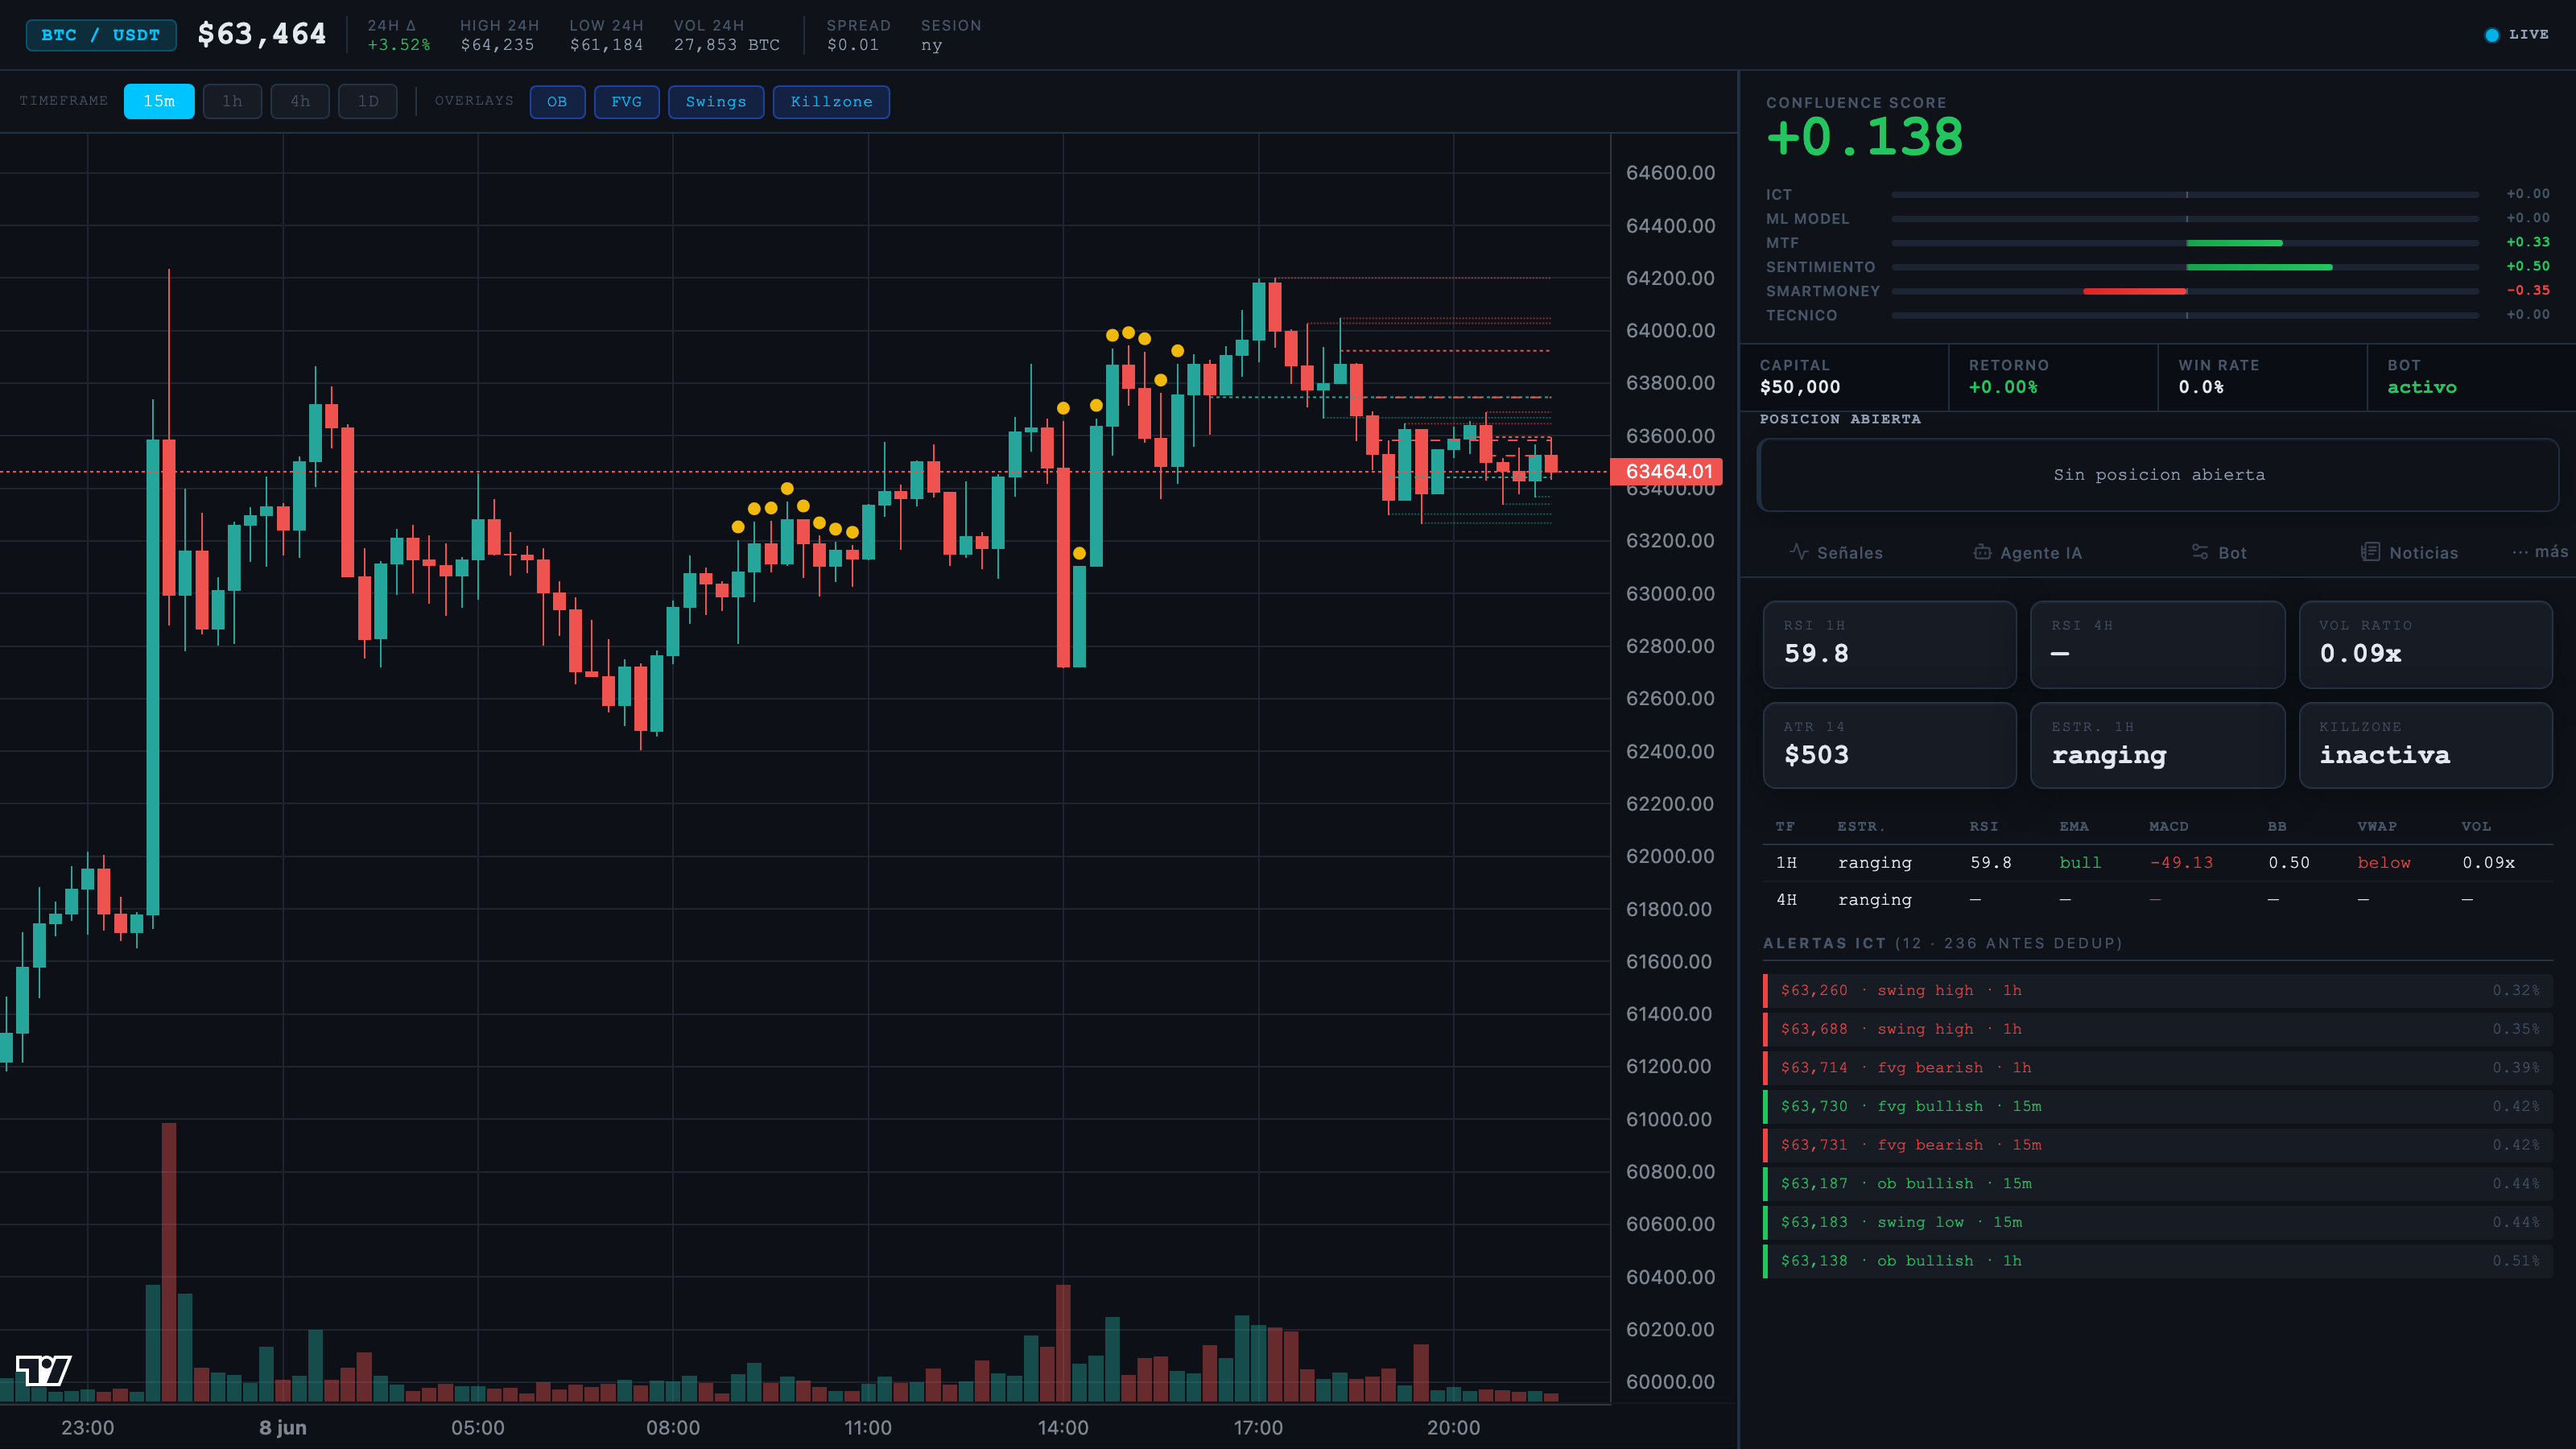
\includegraphics[width=\textwidth]{fig_dashboard_general}
\caption{Vista per defecte del \textit{dashboard} amb la pestanya \textbf{Senyals} activa. S'observa la \textit{topbar} amb el preu \textit{live}, el gràfic principal de TradingView Lightweight Charts amb anotacions ICT, i el panell dret amb el \textit{Signal Hero}, \textit{Capital Strip} i el desglossament dels 6 mòduls del \textit{Confluence Score}.}
\label{fig:dashboardgeneral}
\end{figure}

\begin{figure}[H]
\centering
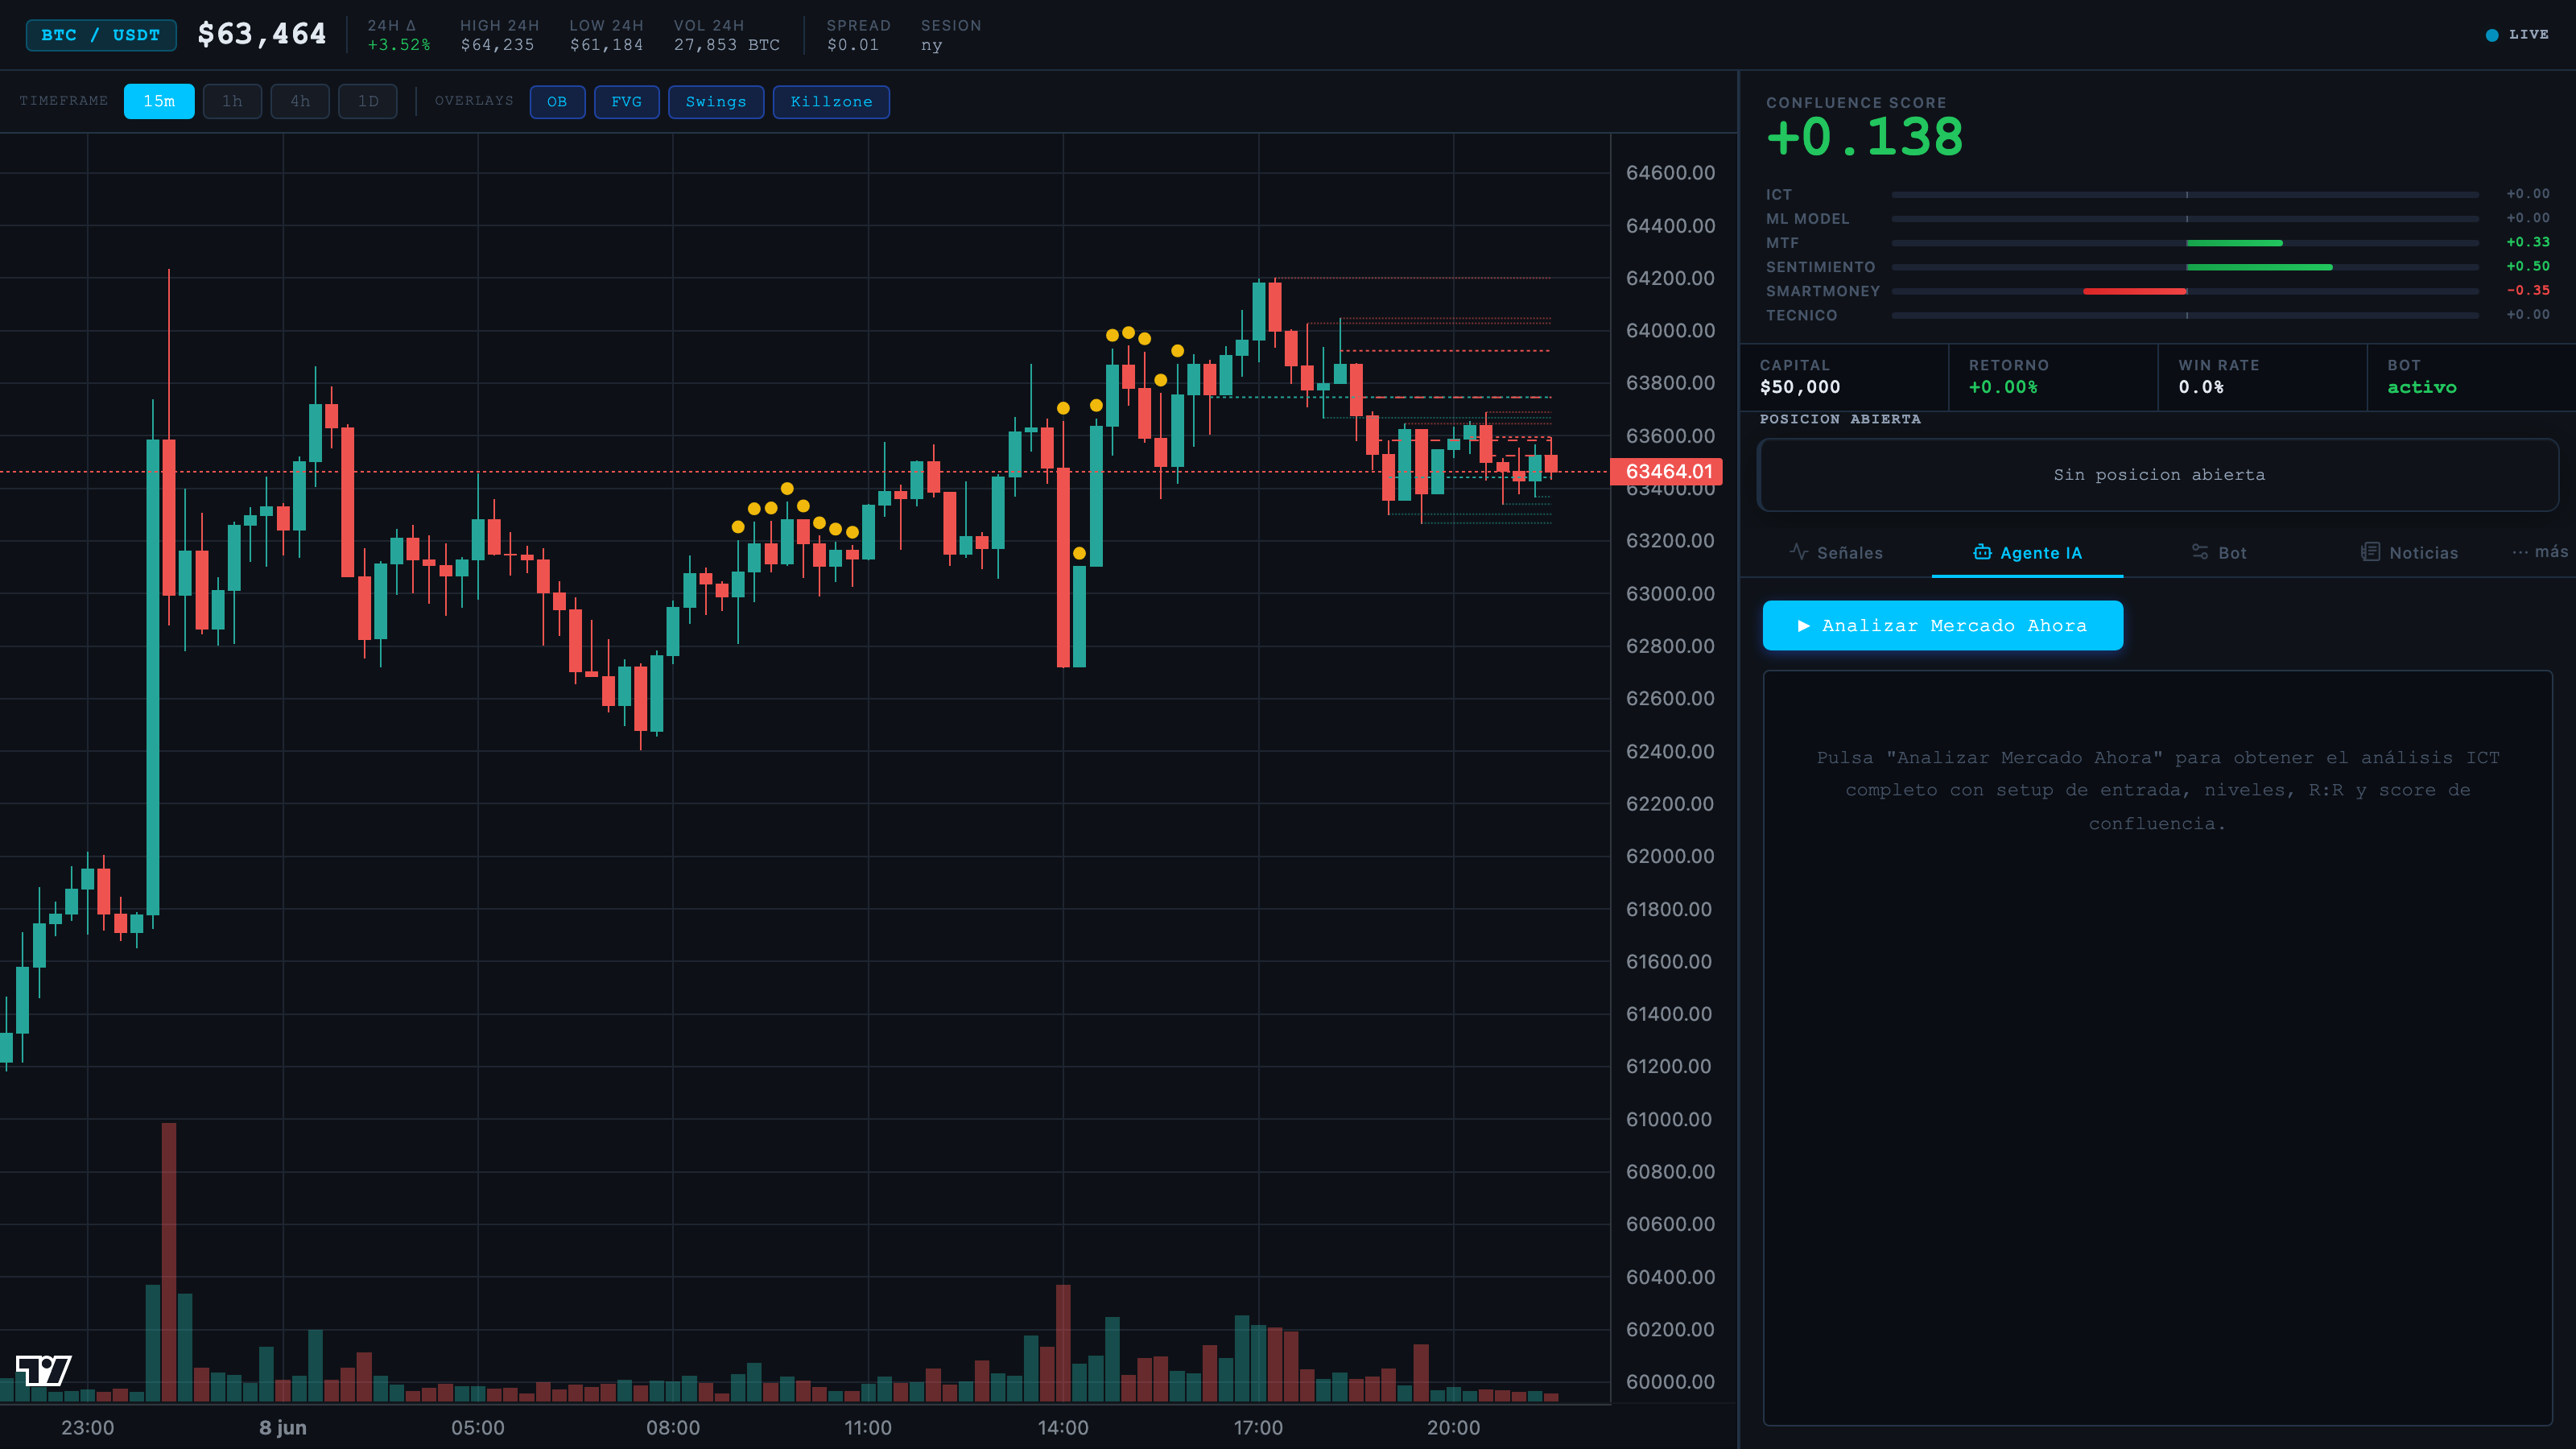
\includegraphics[width=\textwidth]{fig_dashboard_agente}
\caption{Pestanya \textbf{Agente IA}. El botó ``Analizar Mercado'' dispara una crida \textit{streaming} (SSE) al sistema multi-agent sobre GPT-4o: l'Analista retorna l'anàlisi raonada en HTML (amb les eines invocades i el context RAG), el Risk Manager hi afegeix la segona opinió adversarial i el Decision Maker emet la decisió final GO/NO-GO amb el botó d'execució.}
\label{fig:dashboardagente}
\end{figure}

\begin{figure}[H]
\centering
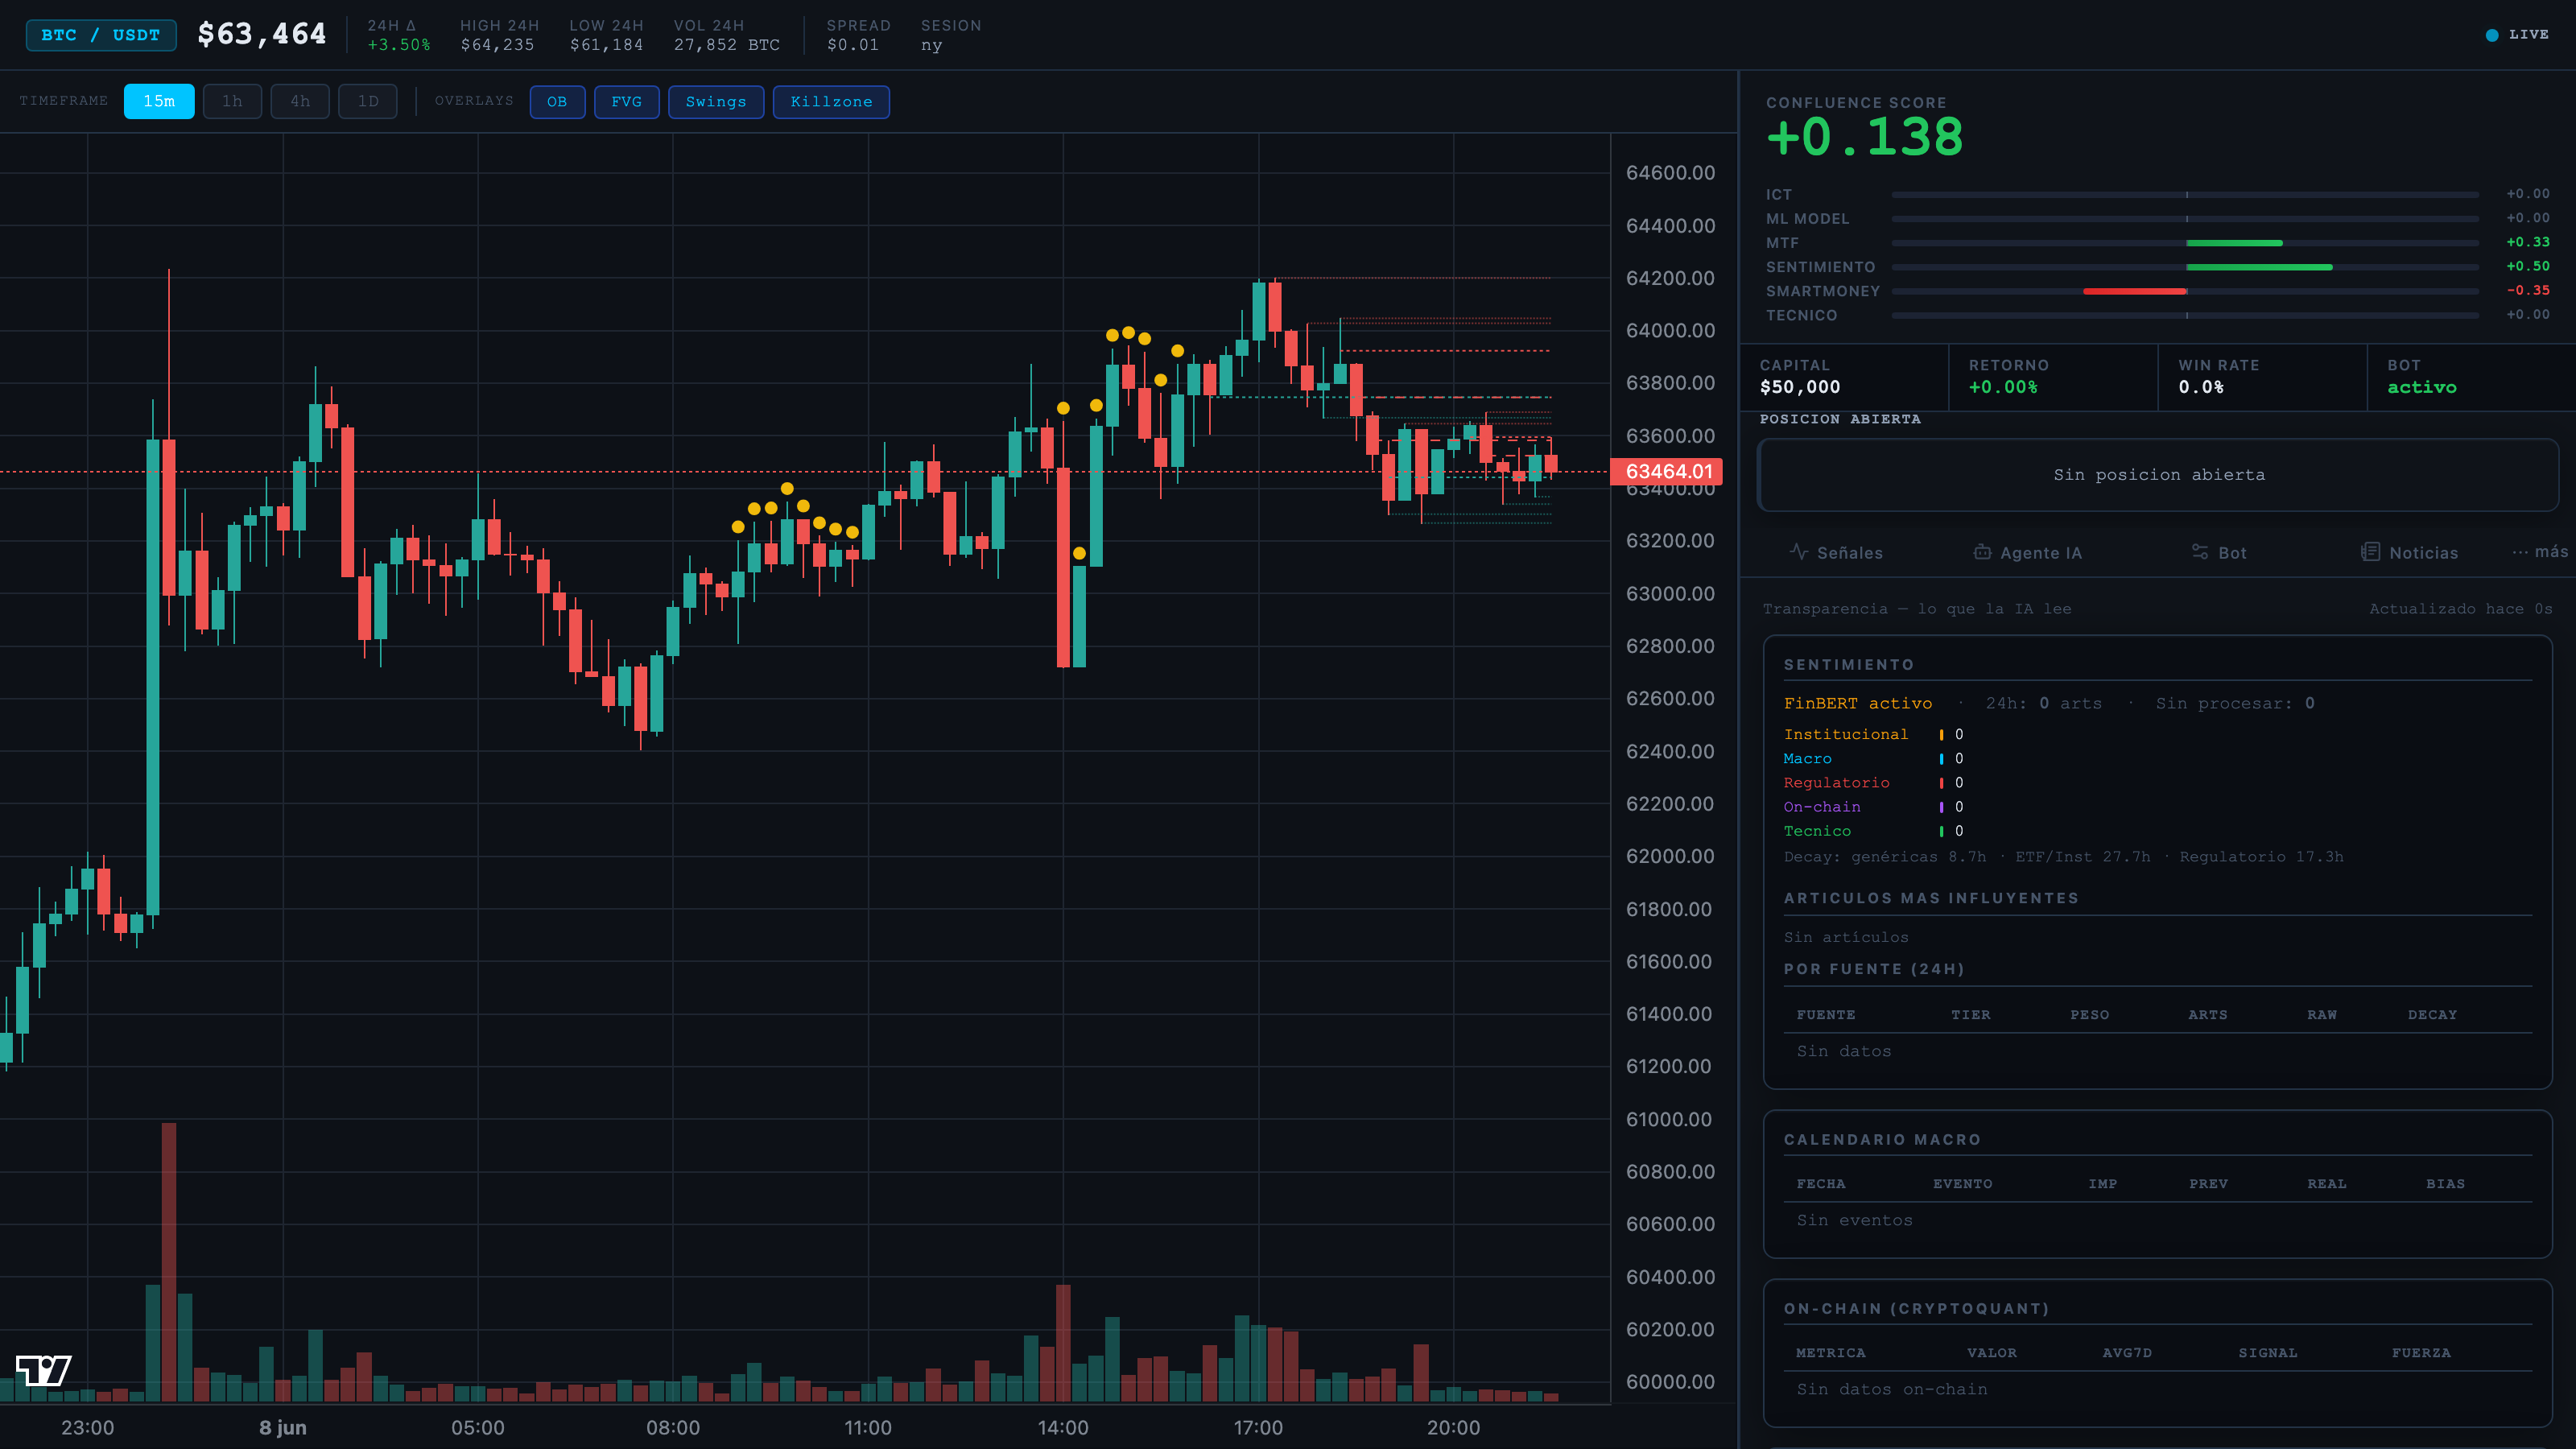
\includegraphics[width=\textwidth]{fig_dashboard_sistema}
\caption{Pestanya \textbf{Sistema} amb els indicadors de \textbf{transparència}: metadades de l'agent, estadístiques del RAG (documents indexats, latència de cerca) i \textit{scores} RAGAS. Aquest tab materialitza el principi de transparència total enunciat a la \S~\ref{cap:dashboard}.}
\label{fig:dashboardsistema}
\end{figure}

\begin{figure}[H]
\centering
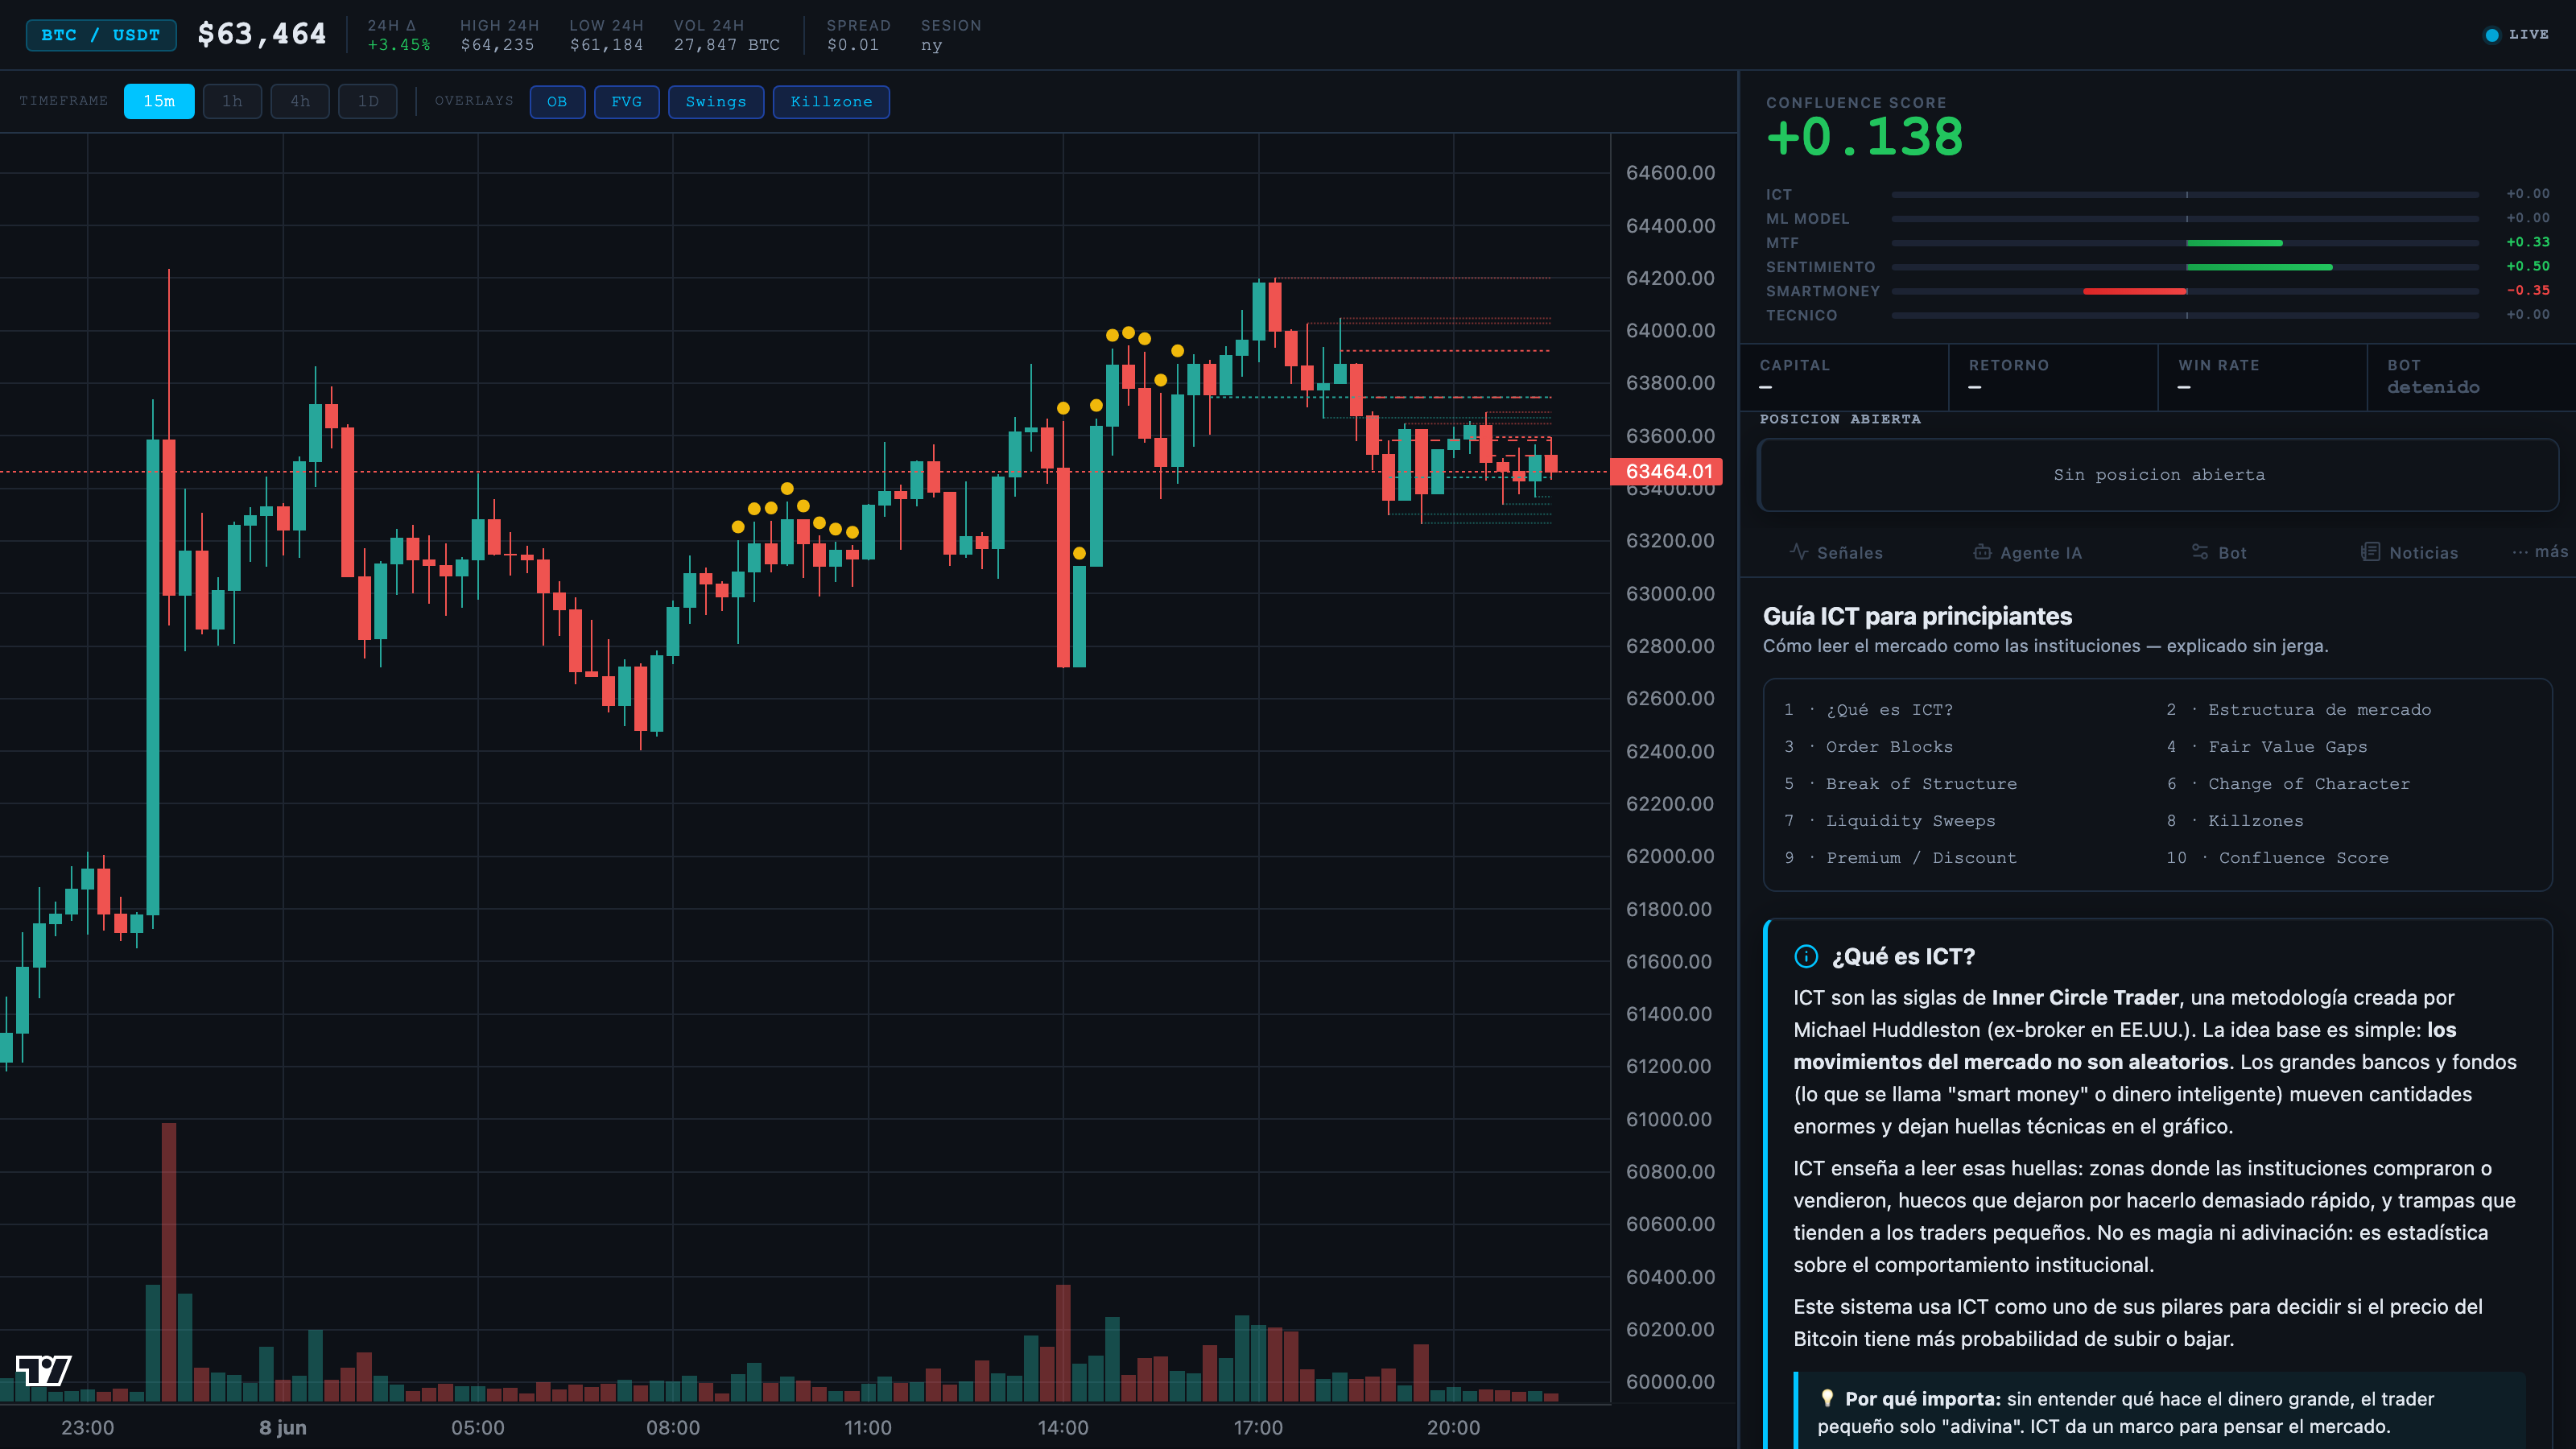
\includegraphics[width=\textwidth]{fig_dashboard_educacion}
\caption{Pestanya \textbf{Educació}, amb la llista de 10 conceptes ICT explicats. Aquest tab fa el \textit{dashboard} comprensible per a usuaris sense formació prèvia en \textit{trading} amb metodologia ICT.}
\label{fig:dashboardeducacion}
\end{figure}

% ------------------------------------------------------------
%  CAPÍTOL 14 — AVALUACIÓ DEL SISTEMA
% ------------------------------------------------------------
\chapter{Avaluació del Sistema}
\label{cap:avaluacio}

El sistema s'ha avaluat per quatre vies complementàries, cadascuna dirigida a un component diferent. La Taula~\ref{tab:resumavaluacio} en resumeix el mapa complet d'evidència.

\begin{table}[H]
\centering
\caption{Mapa d'avaluació del sistema complet}
\label{tab:resumavaluacio}
\begin{tabular}{@{}L{3.2cm}L{3.6cm}L{3.4cm}L{2.6cm}@{}}
\toprule
\textbf{Component} & \textbf{Mètode} & \textbf{Resultat clau} & \textbf{On} \\
\midrule
Models ML & Walk-forward 4$\times$90 + tests & AUC 0,532, \textit{ns} & Cap.~\ref{cap:ml} \\
Estratègia trading & Backtest 360 dies, comissions & Sharpe empitjora amb el llindar & Aquest capítol \\
RAG de l'agent & RAGAS (20 preguntes) & Faithfulness 0,863 & Cap.~\ref{cap:agent} \\
LLM com a filtre (agent únic) & Ablació 365 dies, 500 trucades & $-4{,}5\%$ en \textit{bear} & Cap.~\ref{cap:agent} \\
\bottomrule
\end{tabular}
\end{table}

\section{Backtesting}

\begin{table}[H]
\centering
\caption{Backtest XGBoost + Optuna per llindar de confiança. Període: 2025-03-11 $\to$ 2026-03-05 (360 dies, capital inicial \$10.000, comissió 0.1\%)}
\label{tab:backtest}
\begin{tabular}{@{}rrrrrrr@{}}
\toprule
\textbf{Llindar} & \textbf{Ops} & \textbf{\% mercat} & \textbf{Retorn ML} & \textbf{Retorn B\&H} & \textbf{Sharpe} & \textbf{Max DD} \\
\midrule
0.50 & 69 & 56.9\% & $-13.26\%$ & $-17.83\%$ & $-0.166$ & $-48.71\%$ \\
0.55 & 29 & 16.7\% & $-10.46\%$ & $-17.83\%$ & $-0.216$ & $-32.33\%$ \\
0.60 & 15 &  8.3\% & $-19.53\%$ & $-17.83\%$ & $-0.734$ & $-25.60\%$ \\
0.65 & 15 &  6.1\% & $-24.01\%$ & $-17.83\%$ & $-1.199$ & $-26.14\%$ \\
0.70 &  6 &  2.2\% & $-17.81\%$ & $-17.83\%$ & $-0.967$ & $-19.75\%$ \\
\bottomrule
\end{tabular}
\end{table}

Les Figures~\ref{fig:equity_curve} i~\ref{fig:drawdown} mostren, respectivament, la corba d'\textit{equity} i el \textit{drawdown} acumulat de l'estratègia enfront del \textit{Buy \& Hold}.

% ---- FIG 12: results/figures/fig6_equity_real.png -> fig12_equity_curve.png ----
\begin{figure}[H]
\centering
\includegraphics[width=\textwidth]{fig12_equity_curve}
\caption{Corba d'equity: XGBoost + Optuna ($\theta = 0.50$, blau) vs. Buy \& Hold (vermell), sobre 360 dies de test (2025-03-11 $\to$ 2026-03-05, capital inicial \$10.000, comissió 0.1\%). El període de test va ser majoritàriament baixista (BTC $-17.83\%$). L'estratègia ML perd menys per estar fora del mercat el 43\% del temps, no per capacitat predictiva real.}
\label{fig:equity_curve}
\end{figure}

% ---- FIG 13: results/figures/fig8_drawdown.png -> fig13_drawdown.png ----
\begin{figure}[H]
\centering
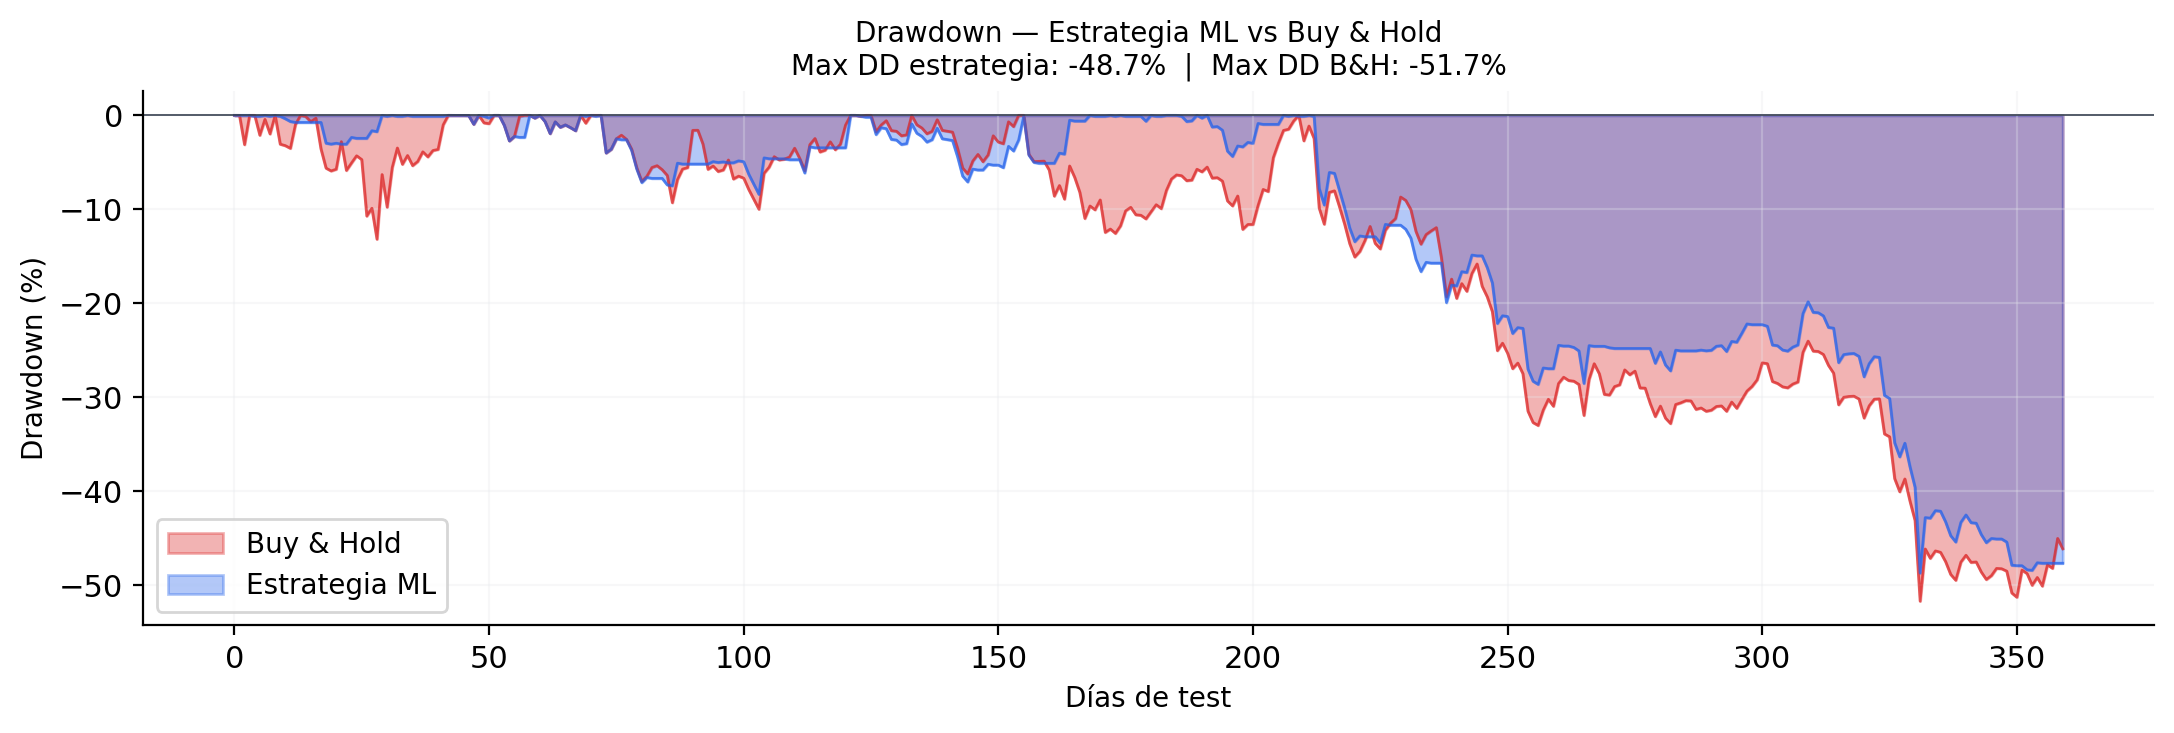
\includegraphics[width=\textwidth]{fig13_drawdown}
\caption{Drawdown acumulat de l'estratègia ML (blau, $\theta = 0.50$) i del Buy \& Hold (vermell) durant els 360 dies de test. El drawdown màxim de l'estratègia és $-48.71\%$ vs $-51.71\%$ del B\&H. La diferència es concentra en els períodes en efectiu (43\% del temps), no en l'encert de les prediccions.}
\label{fig:drawdown}
\end{figure}

\begin{warningbox}[Interpretació crítica del backtest]
La firma estadística d'un model sense senyal real és que el Sharpe \textbf{empitjora} a mesura que augmenta el llindar (de $-0.166$ a $-1.199$ en llindar 0.65). Si el model tingués capacitat predictiva real, esperaríem l'invers: quan el model ``està més segur'', hauria d'encertar més. El que ocorre és l'oposat.
\end{warningbox}

La Figura~\ref{fig:threshold} ho visualitza: el Sharpe i l'exposició al mercat per a cada llindar de decisió.

% ---- FIG 14: results/figures/fig9_threshold_sensitivity.png -> fig14_threshold.png ----
\begin{figure}[H]
\centering
\includegraphics[width=\textwidth]{fig14_threshold}
\caption{Sharpe ratio i exposició al mercat per llindar de decisió (0.50 a 0.70). A mesura que el llindar puja, el model opera menys dies però el Sharpe empitjora (de $-0.166$ a $-1.199$). Aquest patró invers és la signatura estadística d'un model sense senyal predictiva real: si en tingués, exigir més confiança hauria de millorar el Sharpe, no empitjorar-lo.}
\label{fig:threshold}
\end{figure}

% ------------------------------------------------------------
%  CAPÍTOL 15 — ITERACIONS I EVOLUCIÓ
% ------------------------------------------------------------
\chapter{Iteracions i Evolució del Projecte}

\section{Fase inicial (febrer--març 2026): infraestructura}

El projecte va arrencar amb una fase d'investigació bibliogràfica sobre conceptes base: OHLCV, indicadors tècnics, \textit{walk-forward validation}, \textit{data leakage}, \textit{backtesting} sense biaixos. Es va dissenyar l'esquema inicial de quatre taules i es van carregar les dades de preu (65.000+ registres des de 2019).

El problema principal d'aquesta fase va ser la construcció del corpus de notícies: cinc fonts explorades i descartades per raons diverses (Reddit PRAW sense aprovació, CryptoPanic sense historial, GDELT amb \textit{rate limiting} excessiu, NewsAPI sense historial suficient). La solució adoptada va combinar datasets Kaggle amb RSS feeds actius.

\section{Primera etapa de modelatge (març--abril 2026)}

Amb la infraestructura operativa, es van implementar ARIMA, XGBoost i LSTM. L'EDA va revelar que el Fear \& Greed Index era la \textit{feature} més correlacionada amb el \textit{label} (+0.026), seguida dels retorns ($-0.075$, reversió a la mitjana). Els resultats del Seguiment~1 van reportar una millora de +0.015 en AUC en afegir sentiment (de 0.516 a 0.532), interpretada com a ``consistent entre els 5 \textit{splits}''. El problema, detectat posteriorment, és que amb $n = 60$ dies de test per split, l'interval de confiança del AUC és $\pm 0.13$: la millora de 0.015 estava completament dins del marge de soroll estadístic.

La simulació de \textit{trading} del Seguiment~1 va produir un resultat aparentment catastròfic: el model XGBoost va obtenir un retorn de $-81.8\%$ enfront del $+15.8\%$ del Buy \& Hold. L'anàlisi va revelar la causa: amb llindar de decisió de 0.50, el model predeia ``puja'' en només 52 dels 522 dies disponibles, estant fora del mercat el 90\% del temps durant un període majoritàriament alcista. La lliçó va quedar clara (Figura~\ref{fig:trading_sim_seg1}): classificar bé i construir una estratègia rendible són problemes diferents que requereixen optimització separada.

% --- notebooks/figures/07_trading_simulation.png -> fig_trading_sim_seg1.png ---
\begin{figure}[H]
\centering
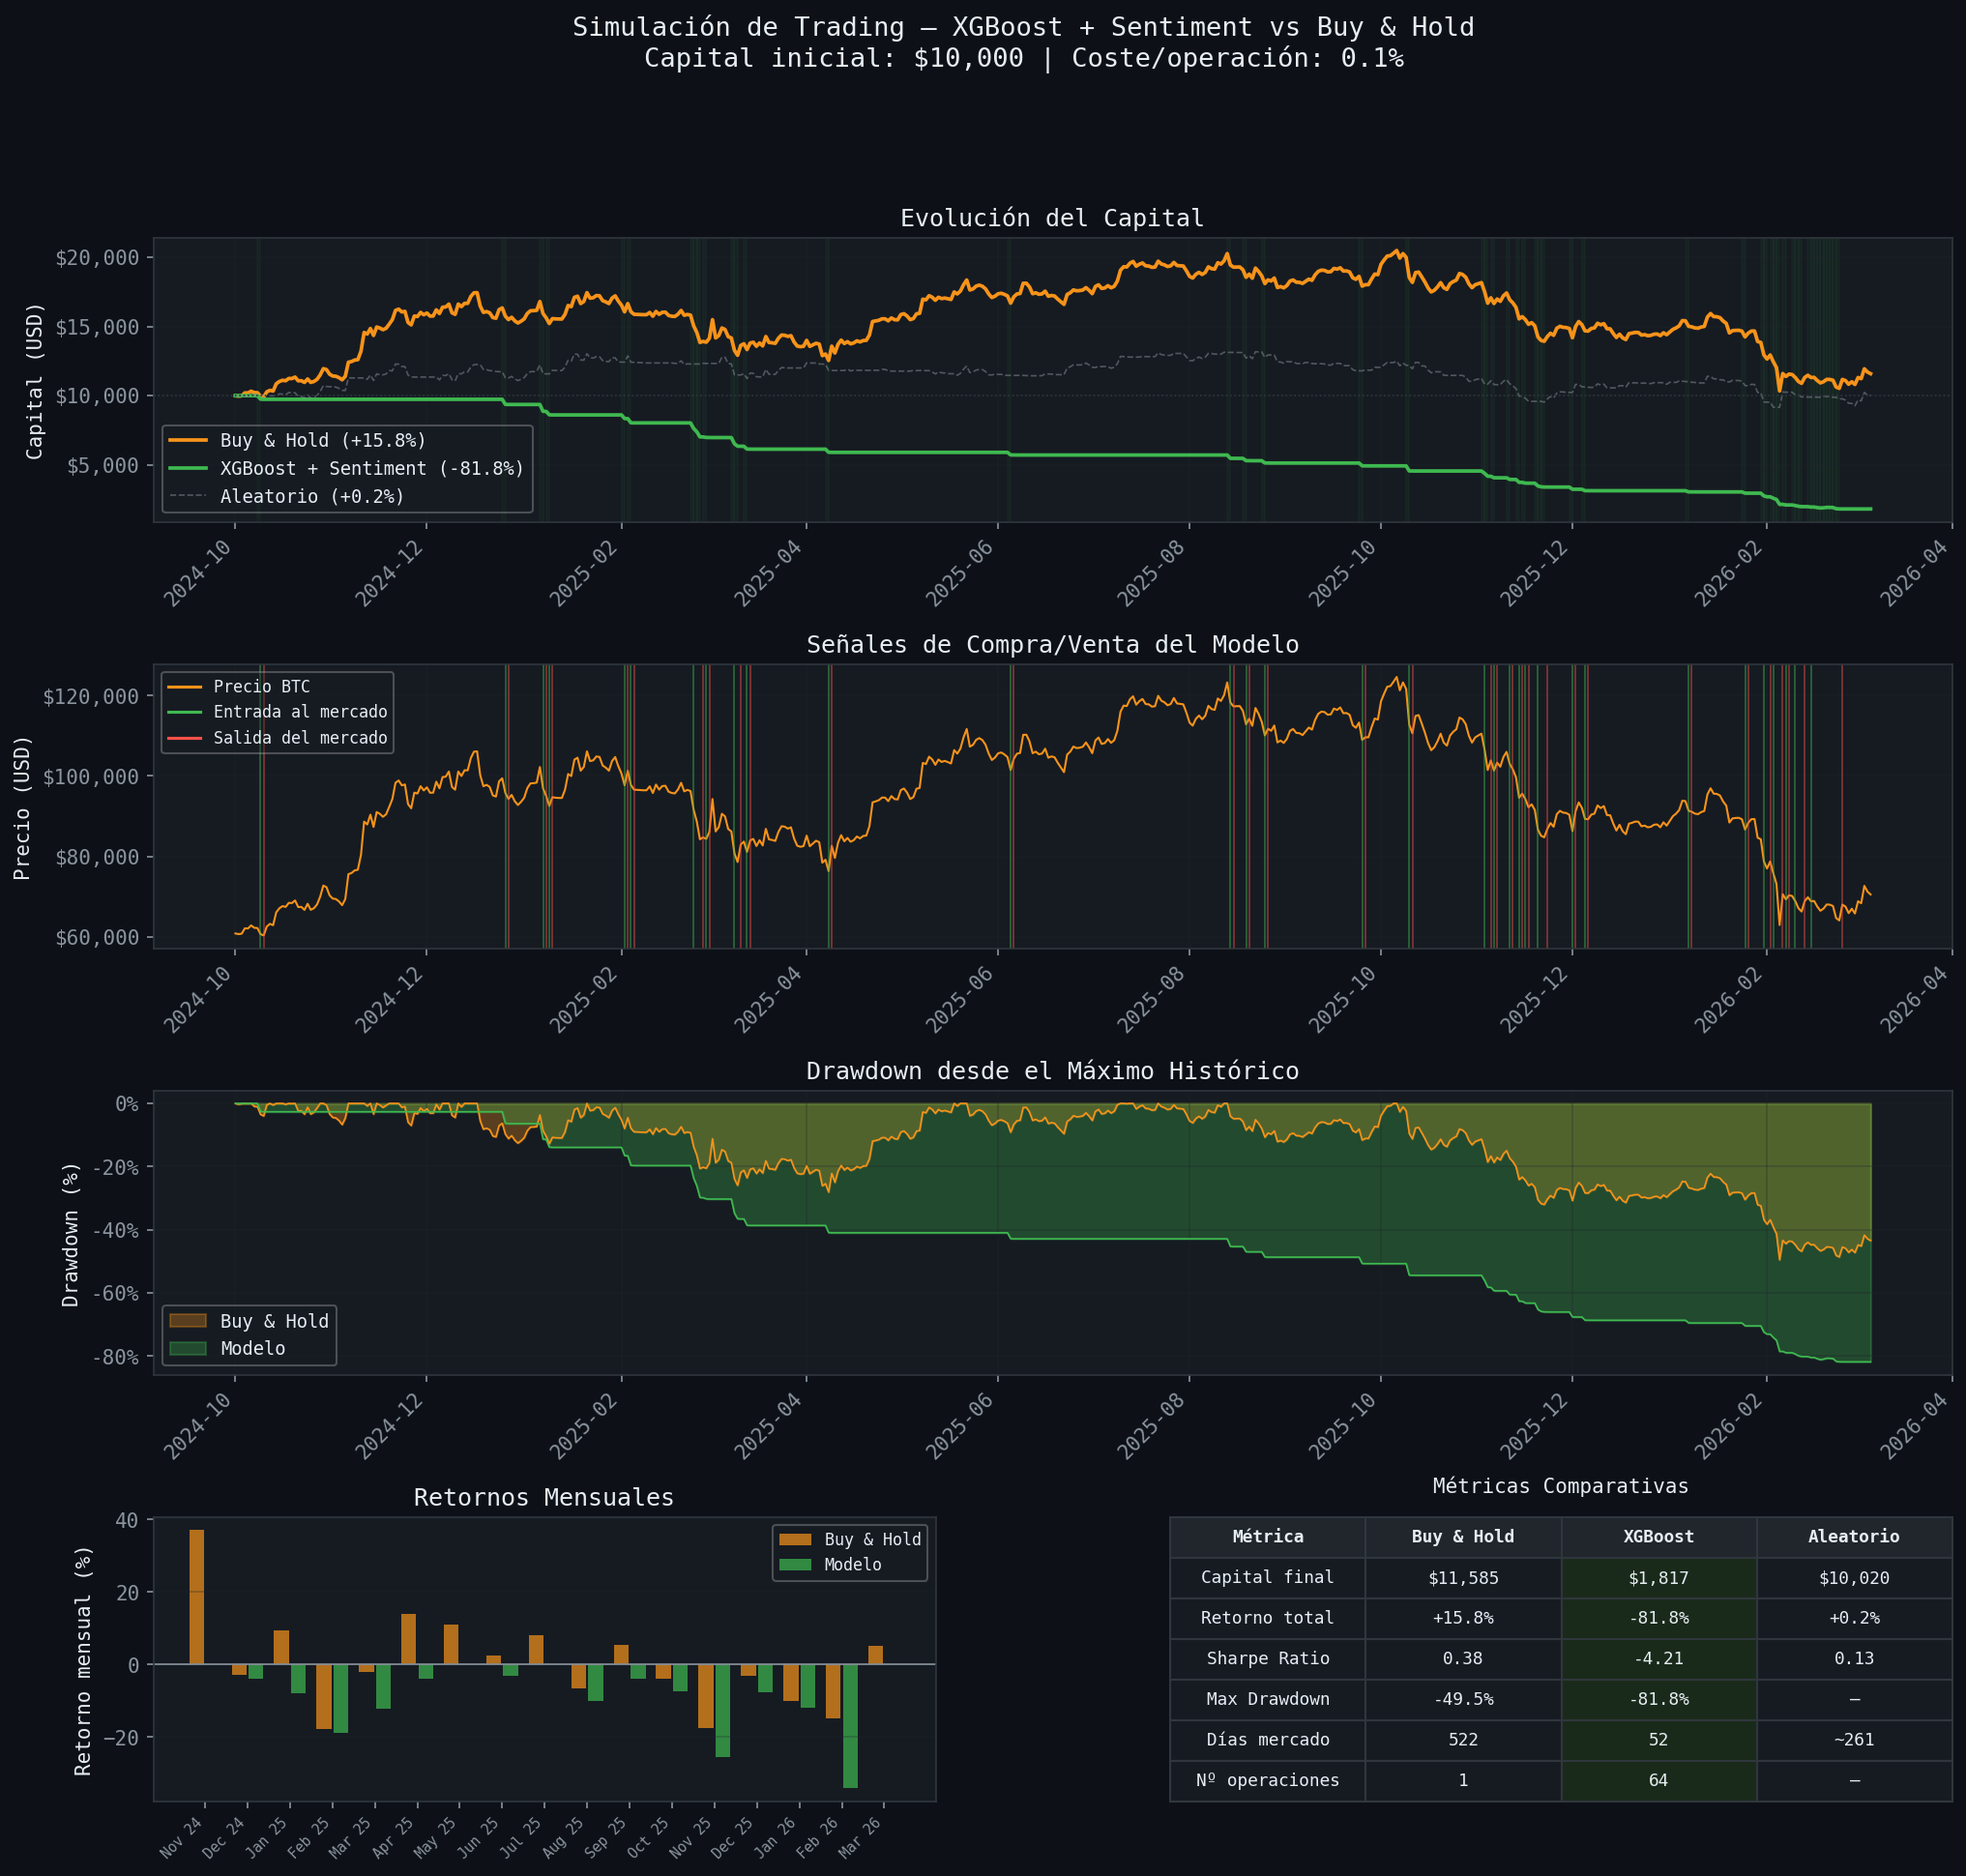
\includegraphics[width=\textwidth]{fig_trading_sim_seg1}
\caption{Simulació de trading del Seguiment~1 (XGBoost + Sentiment, threshold $= 0.50$). El model prediu ``puja'' en només 52 dels 522 dies disponibles (10\% del temps), produint un retorn de $-81.8\%$ enfront del $+15.8\%$ del Buy \& Hold. La causa no és un model dolent: és un llindar de decisió fix que fa que el model estigui fora del mercat el 90\% del temps durant un període majoritàriament alcista. Aquesta figura va motivar l'optimització del llindar en el Seguiment~2.}
\label{fig:trading_sim_seg1}
\end{figure}

\section{Ampliació del corpus i auditoria (abril--juny 2026)}

El període entre Seguiment 1 i Seguiment 2 va ser el més intens del projecte. La decisió crítica va ser auditar el \textit{pipeline} complet, detectant 10 problemes metodològics. En paral\textperiodcentered{}lel, el corpus es va ampliar de 10.438 a 105.125 articles, i la cobertura del sentiment va passar del 34.4\% al 96.2\% dels dies.

Els resultats post-auditoria van confirmar que cap model supera l'atzar amb significança estadística. Aquest resultat, inicialment decebedor, es va reenquadrar ràpidament: és la conclusió correcta i científicament valuosa.

\section{Transició a l'agent d'IA (juny 2026 --- en curs)}

La conclusió de l'etapa ML va obrir la segona fase. En lloc de descartar el treball previ, es va decidir usar-lo com a base d'una arquitectura més rica: un agent d'IA que integra els models ML com a eines de senyal feble dins d'un sistema de raonament més complet.

Aquesta fase ha afegit noves taules (economic\_calendar, institutional\_flows, market\_microstructure, on\_chain\_metrics), ha expandit el \textit{feature set} amb indicadors ICT i ha integrat el \textit{framework} d'anàlisi multi-\textit{timeframe}. El bot de \textit{paper trading} i el \textit{dashboard} ja estan operatius.

A mitjan juny es va fer una auditoria de fiabilitat del sistema en execució contínua (\S~\ref{sec:fiabilitat}) que va corregir cinc defectes d'infraestructura --- fuga de connexions a PostgreSQL, espelma en curs congelada a la ingesta, mitigació de FVGs inoperant, dibuix incorrecte de zones ICT i incoherència de preus entre components --- i va alinear el model ML desplegat amb la versió auditada de la memòria.

\subsection{Evolució final: de l'agent únic al sistema multi-agent (juny 2026)}

L'última fase del treball, documentada de manera incremental al registre de canvis del projecte, va transformar substancialment l'agent. És important per a la lectura dels resultats: les avaluacions quantitatives de retorn (el \textit{backtest} de l'estratègia ML i l'estudi d'ablació) es van fer sobre les configuracions \emph{anteriors} ---el \textit{backtest} avalua el model ML \emph{sense} LLM, i l'ablació, l'agent \emph{únic} com a filtre. El sistema actual, molt més elaborat, és posterior a aquelles mesures. La cronologia d'aquesta evolució final és la següent:

\begin{itemize}[leftmargin=*]
  \item \textbf{Correcció del RAG.} Es va resoldre un conflicte de dependències (TensorFlow/Keras~3) que impedia inicialitzar els \textit{embeddings}; el RAG passa a usar exclusivament PyTorch.
  \item \textbf{Sistema de notícies.} El llistat de notícies del \textit{dashboard} es reordena per data (abans només per influència, cosa que congelava notícies antigues a dalt) i s'afegeix actualització i \textit{scraping} a demanda.
  \item \textbf{De l'agent únic al multi-agent.} L'agent es divideix en tres rols (Analista, Risk Manager i Decision Maker), amb la decisió final GO/NO-GO presa per un \emph{motor de regles determinista} i no pel LLM.
  \item \textbf{Redisseny del Risk Manager.} El model petit (\texttt{gpt-4o-mini}) generava falsos positius en verificar xifres; la solució va ser separar estrictament la verificació (en codi, determinista) de l'opinió (LLM), i migrar \textbf{tots} els rols a \texttt{gpt-4o}.
  \item \textbf{Execució real i control de risc.} Es va connectar el bot per API a Bybit Demo (centralitzant l'execució en un mòdul compartit), afegint \textit{break-even} i \textit{trailing stop} natius, \textit{gating} de l'execució per la decisió GO/NO-GO i límits de cost (5 crides/dia, sense operar caps de setmana).
\end{itemize}

\begin{infobox}[Prova pilot: el primer cicle complet funciona]
Amb tot el sistema en marxa, el bot ---connectat per API--- va \textbf{obrir, gestionar i tancar correctament el seu primer \textit{trade} real} al compte de pràctiques: una posició \textit{long} activada per un \textit{trigger} de nivell, amb \textit{stop loss} i \textit{take profit} natius, tancada de manera controlada. A nivell d'enginyeria, doncs, \emph{tot funciona i està en ordre}: la cadena completa decisió$\to$execució$\to$gestió de risc$\to$registre opera de punta a punta. Ara bé, en ser un treball molt extens i amb el temps esgotat, no s'ha pogut observar el sistema prou dies ni iterar estratègies per saber si \emph{a la llarga} és rendible. Es tracta, doncs, d'una \textbf{prova pilot reeixida}: el sistema està operatiu i validat com a peça d'enginyeria, i la seva avaluació de rendiment a llarg termini queda oberta com a continuació natural.
\end{infobox}

% ------------------------------------------------------------
%  CAPÍTOL 16 — ESTUDI ÈTIC I LEGAL
% ------------------------------------------------------------
\chapter{Estudi Ètic i Legal}

\section{Ús de dades}

Totes les dades del projecte són públiques o estan sota llicències que permeten el seu ús acadèmic. Les dades de preu de Binance són públiques i accessibles sense autenticació. Els datasets Kaggle estan publicats sota llicències Creative Commons. Els \textit{feeds} RSS són públics i el seu \textit{scraping} és legal per a ús no comercial. GDELT és una base de dades pública amb política explícita d'accés obert.

\section{Privadesa i protecció de dades}

El projecte no recopila ni emmagatzema dades personals d'usuaris. Els articles de notícies són text publicat públicament per mitjans de comunicació. El bot de \textit{paper trading} opera exclusivament amb capital virtual a la plataforma demo de Bybit: tot i que envia ordres reals al \textit{matching engine} del compte de pràctiques, no hi ha en cap moment transaccions amb capital real.

\section{Riscos del sistema}

\textbf{Risc de mala interpretació de senyals:} El risc principal és que un usuari interpreti les senyals de l'agent com a prediccions fiables quan en realitat estan dins del soroll estadístic. L'arquitectura de l'agent aborda aquest risc de forma explícita: cada predicció inclou l'AUC històric i l'interval de confiança.

\textbf{Risc d'ús en trading real:} L'agent en el seu estat actual no està dissenyat per a \textit{trading} real. Adaptar-lo requeriria validació addicional, gestió de risc rigorosa i consideracions regulatòries fora de l'abast del TFG.

% ------------------------------------------------------------
%  CAPÍTOL 17 — CONCLUSIONS
% ------------------------------------------------------------
\chapter{Conclusions}

\section{Resposta a la pregunta de recerca}

Aquest treball partia d'una pregunta concreta: \emph{pot un sistema d'aprenentatge automàtic, enriquit amb anàlisi de sentiment de notícies, predir la direcció diària del preu de Bitcoin amb significança estadística?} Després d'una avaluació deliberadament rigorosa, la resposta és \textbf{no}. Cap de les quatre famílies de models supera l'atzar de manera estadísticament significativa (millor AUC = 0,532; $p = 0{,}287$; interval de confiança al 95\% que inclou el 0,5), i l'estratègia de \textit{trading} derivada del millor model perd diners en \textit{backtest} amb costos realistes, amb un Sharpe que \emph{empitjora} a mesura que s'exigeix més confiança al model ---la signatura inequívoca de l'absència de senyal predictiva real. El resultat és consistent amb la forma semi-forta de la hipòtesi d'eficiència de mercat per a un actiu líquid en horitzó diari.

Aquest resultat negatiu, lluny de ser un fracàs, constitueix l'aportació central del treball. En un camp on bona part dels resultats positius publicats no sobreviuen a una auditoria metodològica seriosa, reportar un negatiu verificat val més que un positiu que ningú no ha contrastat.

\section{Contribucions i fil argumental}

Les fases del projecte no són compartiments estancs: s'enllacen en un únic fil conductor ---distingir el senyal real de l'artefacte--- que dona coherència a tot el treball.

\textbf{(1) Infraestructura de dades completa i reproduïble.} PostgreSQL amb 12 taules, 105.125 notícies processades amb FinBERT, 65.466 registres OHLCV i un pipeline automàtic diari. El seu valor transcendeix els resultats dels models: és la base que fa possible tota l'anàlisi posterior i la continuació del treball.

\textbf{(2) El \textit{null finding} i la seva explicació.} El resultat negatiu no es presenta aïllat, sinó explicat per dos elements que li donen sentit. Primer, l'\emph{auditoria de leakage}: una versió del model arribava a un AUC aparent de 0,73 per un \textit{look-ahead bias} en les \textit{features} ICT i, un cop corregit, queia a un honest 0,52 ---una demostració directa de com es fabriquen els falsos positius del camp. Segon, l'\emph{experiment de causalitat inversa}, que mostra que el sentiment de les notícies matinals és més informatiu que l'agregat diari, evidència que bona part del senyal de sentiment de la literatura pot ser un artefacte descriptiu (les notícies expliquen el moviment del dia, no l'anticipen). Tots dos resultats expliquen \emph{per què} apareixen positius espuris i per què els d'aquest treball, un cop nets, són nuls.

\textbf{(3) Resposta estratègica: un sistema d'IA honest, no un oracle.} Acceptat que el model no és un predictor fiable, la segona fase no l'amaga sota un sistema que pretengui batre el mercat: el reutilitza com una \emph{font de senyal feble entre d'altres} (pes del 10\% al \textit{Confluence Score}) dins d'un sistema multi-agent (Analista, Risk Manager i Decision Maker sobre GPT-4o) la decisió final del qual la pren un motor de regles determinista, no el LLM. El sistema integra ML, RAG, microestructura i indicadors ICT i, sobretot, \emph{comunica la seva incertesa} en lloc d'ocultar-la. És una contribució d'enginyeria i de disseny, no una afirmació de rendibilitat.

\section{Sobre el sistema d'IA: què funciona i què encara no es pot afirmar}
\label{sec:concl-agent}

Cal separar dues afirmacions que sovint es confonen: que un sistema \emph{funcioni} a nivell d'enginyeria i que es pugui \emph{demostrar que és rendible}. Aquest treball assoleix la primera i és deliberadament prudent amb la segona, coherentment amb el \textit{null finding} de la primera fase.

\textbf{El que sí es pot afirmar.} El sistema multi-agent està construït i verificat per vies independents: la qualitat del RAG (RAGAS \textit{Faithfulness} 0,863, per sobre del llindar de 0,75); l'auditoria i correcció del \textit{leakage} del model integrat; i, sobretot, la validació \emph{extrem a extrem} del cicle d'execució. En la prova pilot en viu, el bot ---connectat per API a Bybit Demo--- va \textbf{obrir, gestionar i tancar correctament el seu primer \textit{trade} real} (una posició \textit{long} per \textit{trigger} de nivell, amb \textit{stop loss}/\textit{take profit} natius, \textit{break-even} i \textit{trailing stop}). A nivell d'enginyeria, doncs, tot funciona i està en ordre: la cadena decisió$\to$execució$\to$gestió de risc$\to$registre opera de punta a punta.

\textbf{El que (encara) no es pot afirmar.} Que el primer cicle funcioni no vol dir que el sistema sigui \emph{rendible}: són dues coses diferents. Convé situar bé l'evidència de retorn de què es disposa, perquè correspon a \emph{configuracions anteriors}, no al sistema actual: el \textit{backtest} avalua el model ML \emph{sense} LLM (i perd diners), i l'estudi d'ablació avalua l'agent \emph{únic} com a filtre (empitjora un 4,5\% en \textit{bear}). El sistema actual ---triple agent sobre GPT-4o, molt més elaborat--- és posterior a aquelles mesures i \textbf{no s'ha avaluat sobre retorn}, perquè en ser un treball molt extens el temps disponible no ha permès observar-lo prou dies ni iterar estratègies. A més, per construcció, \textbf{no es pot \textit{backtestejar} sense contaminació}: un LLM conté coneixement paramètric del passat, de manera que avaluar-lo sobre dades històriques li dona accés implícit al futur ---un soroll \textit{look-ahead} impossible d'eliminar retrospectivament. I cal ser explícit: un sol \textit{trade} guanyador, per encoratjador que sigui, és estadísticament indistingible de l'atzar; presentar-lo com a prova de rendibilitat seria l'error que aquest treball denuncia. Per tant, el que tenim és una \textbf{prova pilot reeixida} ---el sistema està operatiu i validat com a enginyeria--- i la seva rendibilitat a llarg termini resta com una pregunta oberta que només l'avaluació en viu prolongada podrà respondre.

\begin{infobox}[Una conclusió mesurada]
El sistema d'IA està construït, verificat i operatiu com a peça d'enginyeria i d'investigació. Ara bé, afirmar que ``bat el mercat'' amb les dades disponibles, i encara menys recolzant-se en un grapat d'operacions guanyadores, seria caure en el mateix error que aquest treball retreu a la literatura. La conclusió té dues cares: el sistema \emph{funciona}, però la seva \emph{rendibilitat continua sent una pregunta oberta} que només una avaluació en viu prolongada podrà tancar. Mantenir aquesta exigència en les dues fases del projecte, sense sobrevendre ni el model ni l'agent, és una fortalesa i no una mancança.
\end{infobox}

\section{Compliment dels objectius}

La Taula~\ref{tab:compliment} contrasta cada objectiu específic del Capítol~2 amb l'evidència aportada. Convé una precisió important per llegir-la correctament: els objectius es van formular com a objectius de \emph{recerca i construcció} (dissenyar, implementar, avaluar, investigar), no com la garantia d'obtenir un model predictiu rendible. En aquest sentit s'han assolit tots, \emph{tot i que la resposta empírica a la pregunta predictiva sigui negativa}. Aconseguir l'objectiu de \emph{investigar} si el sentiment aporta valor (OE4) i trobar que no n'aporta de manera significativa no és un incompliment: és, precisament, el resultat de la investigació.

\begin{table}[H]
\centering
\caption{Compliment dels objectius específics}
\label{tab:compliment}
\begin{tabular}{@{}lL{6.2cm}L{4.6cm}@{}}
\toprule
\textbf{OE} & \textbf{Evidència} & \textbf{Estat} \\
\midrule
OE1 & BD de 12 taules + pipeline diari automàtic & \textcolor{accentgreen}{\textbf{Assolit}} \\
OE2 & Corpus de 105.125 textos, cobertura 96,2\% & \textcolor{accentgreen}{\textbf{Assolit}} \\
OE3 & 4 famílies avaluades amb walk-forward + IC 95\% & \textcolor{accentgreen}{\textbf{Assolit}} \\
OE4 & Mann-Whitney $p=0{,}342$ + experiment causalitat inversa & \textcolor{accentgreen}{\textbf{Assolit}} \\
OE5 & Auditoria: 10 problemes corregits + leakage ICT & \textcolor{accentgreen}{\textbf{Assolit}} \\
OE6 & Sistema multi-agent (13 eines) + dashboard + bot amb execució real a Bybit Demo & \textcolor{accentgreen}{\textbf{Assolit}} \\
OE7 & RAGAS: Faithfulness 0,863 sobre 20 preguntes & \textcolor{accentgreen}{\textbf{Assolit}} \\
\bottomrule
\end{tabular}
\end{table}

\section{Aprenentatges i reflexió final}

L'aprenentatge més important d'aquest treball no és tècnic sinó epistemològic: en \textit{machine learning} financer, la dificultat real no és entrenar models ---qualsevol pot obtenir un AUC de 0,73--- sinó \emph{assegurar-se que el número que es reporta és real}. Aquest principi és el que dona unitat a tot el projecte. És el mateix rigor que va fer caure l'AUC de 0,73 a 0,52 en corregir el \textit{leakage}, el que va revelar la causalitat inversa del sentiment, i el que impedeix presentar un grapat d'operacions guanyadores de l'agent com una prova de rendibilitat. La temptació, a cada fase, era acceptar el resultat afalagador; la decisió, a cada fase, va ser verificar-lo i, sovint, desautoritzar-lo.

El treball deixa, doncs, una doble herència. D'una banda, una \emph{conclusió científica}: per a Bitcoin en horitzó diari, amb les dades públiques disponibles, no hi ha senyal predictiva explotable de manera significativa ---un resultat negatiu però honest i alineat amb l'eficiència de mercat. De l'altra, una \emph{infraestructura d'enginyeria} completa i un sistema multi-agent operatiu que, sense pretendre batre el mercat, estructura el procés d'anàlisi i comunica la seva pròpia incertesa. Tots dos llegats convergeixen en la mateixa lliçó: en finances quantitatives, l'honestedat metodològica no és un afegit ètic, sinó la condició mateixa de la validesa dels resultats.

% ------------------------------------------------------------
%  CAPÍTOL 18 — LÍNIES FUTURES
% ------------------------------------------------------------
\chapter{Línies Futures}

\begin{enumerate}
  \item \textbf{Major poder estadístic:} Treballar amb dades horàries o de 4h en lloc de diàries, per tenir $n > 50$ \textit{splits} i poder estadístic $> 80\%$.

  \item \textbf{Models de règim:} Entrenar un model de canvi de règim (Hidden Markov Model) que identifiqui el règim actual i seleccioni el model ML més adequat.

  \item \textbf{Senyals de sentiment granulars:} Classificar notícies per hora de publicació, tipus de font i categoria temàtica (regulació, adopció, macroeconomia).

  \item \textbf{Ampliació de l'avaluació RAGAS:} Estendre el test set de 20 a 100+ preguntes, incorporar preguntes adversarials i avaluar amb un segon LLM-as-judge per mesurar la robustesa de les mètriques.

  \item \textbf{Multi-actiu:} Estendre el sistema a Ethereum, S\&P 500 i or per comparar el nivell d'eficiència de mercat entre classes d'actius.

  \item \textbf{Memòria persistent:} Dotar l'agent de capacitat d'aprenentatge continu a partir dels seus propis errors.
\end{enumerate}

% ------------------------------------------------------------
%  APÈNDIXS
% ------------------------------------------------------------
\appendix

\chapter{Verificació de Target Leakage}

\begin{lstlisting}[style=python, caption={Test de verificacio de target leakage (statistical\_tests.py)}]
from scipy.stats import pearsonr

def verify_no_target_leakage(df, tolerance=(-0.1, -0.05)):
    """
    Verifica que label_t codifica el dia seguent, no l'actual.
    Si label_t = 1 quan Close_{t+1} > Close_t, aleshores:
    - corr(returns_t, label_t) ha de ser negativa (reversio a la mitj.)
    - El valor esperat es ~-0.07 per BTC en horitz. diari
    """
    r, p = pearsonr(df['returns'], df['label'])
    assert tolerance[0] < r < tolerance[1], \
        f"Possible target leakage: r={r:.4f} fora de {tolerance}"
    print(f"OK: corr(returns, label) = {r:.4f}  (p={p:.4f})")
    return r

# Resultat: corr(returns_t, label_t) = -0.0725  OK
\end{lstlisting}

\chapter{Walk-forward amb Gap Temporal}

\begin{lstlisting}[style=python, caption={Configuracio walk-forward amb embargament (data\_loader.py)}]
def get_walk_forward_splits(df, n_splits=4, test_size=90, gap=7):
    """
    Walk-forward validation amb gap temporal (purging).
    El gap impedeix que features amb finestra movil contaminin el test.
    
    Parametres:
      n_splits   : nombre de splits (4 per defecte)
      test_size  : dies de test per split (90 per defecte)
      gap        : embargament entre train i test (7 dies)
    """
    splits = []
    n = len(df)
    for i in range(n_splits):
        test_end   = n - i * test_size
        test_start = test_end - test_size
        train_end  = test_start - gap   # embargament temporal
        train_idx  = df.index[:train_end]
        test_idx   = df.index[test_start:test_end]
        splits.append((train_idx, test_idx))
    return splits[::-1]   # ordre cronologic
\end{lstlisting}

\chapter{Resum Estadístic del Dataset ML}

\begin{table}[H]
\centering
\caption{Estadística descriptiva de daily\_features (2019-01-01 a 2026-06-03)}
\label{tab:estadistica}
\begin{tabular}{@{}lr@{}}
\toprule
\textbf{Mètrica} & \textbf{Valor} \\
\midrule
Observacions totals              & 2.711 \\
Dies alcistes (label=1)          & 1.382 (51.0\%) \\
Dies baixistes (label=0)         & 1.329 (49.0\%) \\
Cobertura sentiment FinBERT      & 2.607 / 2.711 (96.2\%) \\
RSI-14 (mitjana)                 & 52.83 \\
RSI-14 (rang)                    & [15.04, 89.99] \\
Sentiment FinBERT (mitjana)      & $+0.0172$ \\
Sentiment FinBERT (std)          & 0.1992 \\
Fear \& Greed (mitjana)          & 47.6 \\
Retorns diaris (std)             & 3.1\% \\
Volatilitat anualitzada          & $\approx 53\%$ \\
\midrule
\multicolumn{2}{l}{\textit{Distribució anual de dies alcistes}} \\
2019 & 52\% \\
2020 & 58\% \\
2021 & 50\% \\
2022 & 46\% \\
2023 & 50\% \\
2024 & 52\% \\
2025 & 50\% \\
2026 & 47\% \\
\bottomrule
\end{tabular}
\end{table}

\chapter{Preguntes freqüents }

\section*{Sobre la metodologia ML}

\textbf{P: Per què walk-forward i no k-fold estàndard?}
R: El k-fold estàndard és inaplicable a sèries temporals perquè pot incorporar informació futura en l'entrenament (\textit{data leakage}). En cada \textit{fold} de k-fold, el model pot entrenar-se amb dades posteriors al conjunt de test. Walk-forward garanteix que el model mai accedeixi a dades futures.

\textbf{P: Per què 4 splits de 90 dies i no més splits?}
R: Amb 4 splits, el poder estadístic per detectar $\Delta$AUC = 0.05 és del 18\%. Idealment necessitaríem 50+ splits, però amb dades diàries i un dataset de 7 anys, 4 splits de 90 dies és el millor compromís entre mida del test (IC del AUC) i nombre de splits. Per tenir 50+ splits caldria treballar amb dades horàries.

\textbf{P: Per què XGBoost i no un transformer o model més modern?}
R: XGBoost és el model de referència en \textit{tabular data} amb features heterogènies i datasets de mida moderada (2.711 files). Els transformers requereixen ordres de magnitud més dades per superar models d'arbres en dades tabulars, cosa que múltiples estudis (\textit{TabPFN}, \textit{Why do tree-based models still outperform deep learning on tabular data?}) confirmen.

\textbf{P: Qué significa que p = 0.287?}
R: Significa que, assumint que el model no prediu millor que l'atzar (H0: AUC = 0.5), hi hauria un 28.7\% de probabilitat d'observar un AUC tan extrem com el que hem obtingut. Per rebutjar H0 necessitem p < 0.05. Un p = 0.287 no ens permet afirmar que el model prediu millor que l'atzar.

\textbf{P: Un resultat nul és realment un resultat vàlid?}
R: Sí, i és la resposta correcta davant de la pregunta de recerca. Un resultat que confirma empíricament el que la teoria econòmica prediu (eficiència semi-forta del mercat) és tan vàlid com un resultat positiu. La diferència és que és honest: molts papers del camp reportarien AUC = 0.55 com a ``positiu'' sense verificar-ne la significança estadística.

\section*{Sobre el sentiment i la causalitat}

\textbf{P: Per què afegir FinBERT complet empitjora el AUC?}
R: Perquè el corpus conté notícies publicades \textit{després} que el preu s'ha mogut. Una notícia de les 22:00 que diu ``Bitcoin puja un 5\% avui'' té sentiment positiu però no és predictiva: descriu un moviment ja ocorregut. Agregar aquest sentiment al del dia contamina la senyal. L'experiment \textit{morning} vs. \textit{full} confirma que les notícies matinals (publicades abans que el mercat reaccioni) tenen AUC sistemàticament superior.

\textbf{P: El Mann-Whitney p = 0.342 que significa exactament?}
R: Que les distribucions del sentiment FinBERT en dies alcistes i en dies baixistes són estadísticament indistingibles. És la prova més directa i independent de qualsevol model ML: si el sentiment tingués poder predictiu, esperaríem que fos, de mitjana, més positiu els dies que el mercat puja l'endemà. No ho és.

\section*{Sobre l'agent d'IA}

\textbf{P: Per què usar un LLM si els models ML no prediuen?}
R: Precisament perquè no prediuen en el sentit clàssic. L'agent no intenta ``millorar'' el AUC. El seu valor és diferent: integra senyals heterogènies (ML, microestructura, macroeconomia, ETFs, on-chain), raona sobre el context actual del mercat, i comunica l'anàlisi amb incertesa explícita. Un analista humà faria el mateix: no ``prediu'' el preu, sinó que descriu el context i les probabilitats condicionals.

\textbf{P: Com evites que el RAG ``llegeixi'' notícies futures?}
R: El retrieval aplica un filtre temporal estricte: \texttt{WHERE timestamp < data\_consulta}. Quan l'agent raona sobre una data passada, la cerca semàntica sobre l'índex FAISS només retorna documents publicats \textit{abans} d'aquella data.

\textbf{P: Com avalues la qualitat de l'agent?}
R: Amb el framework RAGAS, que mesura tres dimensions: \textit{Faithfulness} (les afirmacions de la resposta estan recolzades pels documents recuperats?), \textit{Answer Relevancy} (la resposta és rellevant per a la pregunta?) i \textit{Context Precision} (els documents recuperats són els més rellevants disponibles?). L'avaluació s'ha completat amb un test set de 20 preguntes en 5 categories (Faithfulness 0,863); l'ampliació del test set és una línia de treball futur.

\textbf{P: Per què tres agents i no un de sol?}
R: Perquè un únic LLM que alhora analitza i s'autoaudita barreja dues tasques de naturalesa diferent: la verificació (determinista, que hauria de ser codi) i el judici (qualitatiu, propi d'un LLM). En la pràctica, l'agent únic generava falsos positius en revisar xifres. La solució va ser separar els rols: l'Analista genera, el Risk Manager audita amb verificació en codi i el Decision Maker decideix amb un motor de regles determinista. El LLM només aporta el component qualitatiu; el GO/NO-GO és reproduïble.

\textbf{P: El sistema guanya diners?}
R: No es pot afirmar amb les dades disponibles, i seria un error metodològic dir que sí. La prova pilot en viu demostra que el cicle complet (decisió, execució, gestió de risc, tancament) \emph{funciona} a nivell d'enginyeria, i el primer \textit{trade} real es va executar correctament. Però un grapat d'operacions és estadísticament indistingible de l'atzar, el \textit{backtest} de les configuracions anteriors perd diners, i un sistema basat en LLM no es pot \textit{backtestejar} sense contaminació \textit{look-ahead}. La rendibilitat només es podrà afirmar (o descartar) amb una avaluació en viu de mesos.

\section*{Sobre el sistema en general}

\textbf{P: Per què usar PostgreSQL i no una base de dades vectorial com Pinecone o Chroma?}
R: El disseny original utilitzava pgvector, l'extensió vectorial nativa de PostgreSQL, per mantenir tota la infraestructura sota un únic motor. Problemes persistents d'instal·lació en l'entorn local (incompatibilitats de versions amb mòduls compilats) van motivar la migració a FAISS per a la capa de cerca semàntica, tal com es documenta al Capítol de disseny de l'agent. Per al volum actual (1.996 documents, vectors de 384 dimensions), FAISS amb cerca exacta és suficient i evita la complexitat operacional d'un servei vectorial extern com Pinecone o Chroma.

\textbf{P: El sistema podria estendre's a altres actius?}
R: Sí. L'esquema de la base de dades inclou la columna \texttt{asset} com a part de la clau primària de \texttt{price\_data} i \texttt{daily\_features}. Afegir Ethereum o S\&P 500 requeriria únicament un nou \textit{fetcher} de preus i adaptar les fonts de notícies. L'arquitectura de l'agent no canviaria.

% ------------------------------------------------------------
%  BIBLIOGRAFIA
% ------------------------------------------------------------
\begin{thebibliography}{99}
\bibitem{fama1970}
  E.~F. Fama, ``Efficient Capital Markets: A Review of Theory and Empirical Work,''
  \textit{The Journal of Finance}, vol.~25, no.~2, pp.~383--417, 1970.

\bibitem{liu2020}
  Y.~Liu et al., ``FinBERT: A Pre-trained Financial Language Representation Model for Financial Text Mining,''
  in \textit{Proc. IJCAI}, 2020.

\bibitem{fischer2018}
  T.~Fischer and C.~Krauss, ``Deep learning with long short-term memory networks for financial market predictions,''
  \textit{European Journal of Operational Research}, vol.~270, no.~2, pp.~654--669, 2018.

\bibitem{sezer2020}
  O.~B. Sezer, M.~U. Gudelek, and A.~M. Ozbayoglu, ``Financial time series forecasting with deep learning: A systematic literature review,''
  \textit{Applied Soft Computing}, vol.~90, p.~106074, 2020.

\bibitem{bollen2011}
  J.~Bollen, H.~Mao, and X.~Zeng, ``Twitter mood predicts the stock market,''
  \textit{Journal of Computational Science}, vol.~2, no.~1, pp.~1--8, 2011.

\bibitem{sebastiao2021}
  H.~Sebastião and P.~Godinho, ``Forecasting and trading cryptocurrencies with machine learning under changing market conditions,''
  \textit{Financial Innovation}, vol.~7, no.~1, pp.~1--30, 2021.

\bibitem{uras2020}
  N.~Uras et al., ``Forecasting Bitcoin closing price series using linear regression and neural networks models,''
  \textit{PeerJ Computer Science}, vol.~6, p.~e279, 2020.

\bibitem{lopezdeprado2018}
  M.~López de Prado, \textit{Advances in Financial Machine Learning}. Wiley, 2018.

\bibitem{es2024}
  S.~Es et al., ``RAGAS: Automated Evaluation of Retrieval Augmented Generation,''
  in \textit{Proc. EACL}, 2024.

\bibitem{lewis2020}
  M.~Lewis et al., ``Retrieval-Augmented Generation for Knowledge-Intensive NLP Tasks,''
  in \textit{Proc. NeurIPS}, 2020.

\bibitem{xiong2024}
  M.~Xiong et al., ``Can LLMs Express Their Uncertainty? An Empirical Evaluation of Confidence Elicitation in Large Language Models,''
  \textit{arXiv preprint arXiv:2306.13063}, 2024.

\bibitem{urquhart2016}
  A.~K. Urquhart, ``The inefficiency of Bitcoin,''
  \textit{Economics Letters}, vol.~148, pp.~80--82, 2016.

\bibitem{chen2016}
  T.~Chen and C.~Guestrin, ``XGBoost: A Scalable Tree Boosting System,''
  in \textit{Proc. ACM KDD}, pp.~785--794, 2016.

\bibitem{stockbench2025}
  Y.~Lin et al., ``StockBench: Can LLM Agents Trade Stocks Profitably in Real-World Markets?,''
  \textit{arXiv preprint arXiv:2510.02209}, 2025.

\bibitem{yao2023react}
  S.~Yao et al., ``ReAct: Synergizing Reasoning and Acting in Language Models,''
  in \textit{Proc. ICLR}, 2023.

\bibitem{xiao2024tradingagents}
  Y.~Xiao et al., ``TradingAgents: Multi-Agents LLM Financial Trading Framework,''
  \textit{arXiv preprint arXiv:2412.20138}, 2024.

\bibitem{yu2023finmem}
  Y.~Yu et al., ``FinMem: A Performance-Enhanced LLM Trading Agent with Layered Memory and Character Design,''
  \textit{arXiv preprint arXiv:2311.13743}, 2023.

\bibitem{zhang2024finagent}
  W.~Zhang et al., ``A Multimodal Foundation Agent for Financial Trading: Tool-Augmented, Diversified, and Generalist,''
  in \textit{Proc. ACM SIGKDD}, 2024.

\bibitem{du2023debate}
  Y.~Du, S.~Li, A.~Torralba, J.~B. Tenenbaum, and I.~Mordatch, ``Improving Factuality and Reasoning in Language Models through Multiagent Debate,''
  \textit{arXiv preprint arXiv:2305.14325}, 2023.
\end{thebibliography}

\end{document}
